\documentclass[twoside]{book}

% Packages required by doxygen
\usepackage{fixltx2e}
\usepackage{calc}
\usepackage{doxygen}
\usepackage[export]{adjustbox} % also loads graphicx
\usepackage{graphicx}
\usepackage[utf8]{inputenc}
\usepackage{makeidx}
\usepackage{multicol}
\usepackage{multirow}
\PassOptionsToPackage{warn}{textcomp}
\usepackage{textcomp}
\usepackage[nointegrals]{wasysym}
\usepackage[table]{xcolor}

% Font selection
\usepackage[T1]{fontenc}
\usepackage[scaled=.90]{helvet}
\usepackage{courier}
\usepackage{amssymb}
\usepackage{sectsty}
\renewcommand{\familydefault}{\sfdefault}
\allsectionsfont{%
  \fontseries{bc}\selectfont%
  \color{darkgray}%
}
\renewcommand{\DoxyLabelFont}{%
  \fontseries{bc}\selectfont%
  \color{darkgray}%
}
\newcommand{\+}{\discretionary{\mbox{\scriptsize$\hookleftarrow$}}{}{}}

% Page & text layout
\usepackage{geometry}
\geometry{%
  a4paper,%
  top=2.5cm,%
  bottom=2.5cm,%
  left=2.5cm,%
  right=2.5cm%
}
\tolerance=750
\hfuzz=15pt
\hbadness=750
\setlength{\emergencystretch}{15pt}
\setlength{\parindent}{0cm}
\setlength{\parskip}{3ex plus 2ex minus 2ex}
\makeatletter
\renewcommand{\paragraph}{%
  \@startsection{paragraph}{4}{0ex}{-1.0ex}{1.0ex}{%
    \normalfont\normalsize\bfseries\SS@parafont%
  }%
}
\renewcommand{\subparagraph}{%
  \@startsection{subparagraph}{5}{0ex}{-1.0ex}{1.0ex}{%
    \normalfont\normalsize\bfseries\SS@subparafont%
  }%
}
\makeatother

% Headers & footers
\usepackage{fancyhdr}
\pagestyle{fancyplain}
\fancyhead[LE]{\fancyplain{}{\bfseries\thepage}}
\fancyhead[CE]{\fancyplain{}{}}
\fancyhead[RE]{\fancyplain{}{\bfseries\leftmark}}
\fancyhead[LO]{\fancyplain{}{\bfseries\rightmark}}
\fancyhead[CO]{\fancyplain{}{}}
\fancyhead[RO]{\fancyplain{}{\bfseries\thepage}}
\fancyfoot[LE]{\fancyplain{}{}}
\fancyfoot[CE]{\fancyplain{}{}}
\fancyfoot[RE]{\fancyplain{}{\bfseries\scriptsize Generated by Doxygen }}
\fancyfoot[LO]{\fancyplain{}{\bfseries\scriptsize Generated by Doxygen }}
\fancyfoot[CO]{\fancyplain{}{}}
\fancyfoot[RO]{\fancyplain{}{}}
\renewcommand{\footrulewidth}{0.4pt}
\renewcommand{\chaptermark}[1]{%
  \markboth{#1}{}%
}
\renewcommand{\sectionmark}[1]{%
  \markright{\thesection\ #1}%
}

% Indices & bibliography
\usepackage{natbib}
\usepackage[titles]{tocloft}
\setcounter{tocdepth}{3}
\setcounter{secnumdepth}{5}
\makeindex

% Hyperlinks (required, but should be loaded last)
\usepackage{ifpdf}
\ifpdf
  \usepackage[pdftex,pagebackref=true]{hyperref}
\else
  \usepackage[ps2pdf,pagebackref=true]{hyperref}
\fi
\hypersetup{%
  colorlinks=true,%
  linkcolor=blue,%
  citecolor=blue,%
  unicode%
}

% Custom commands
\newcommand{\clearemptydoublepage}{%
  \newpage{\pagestyle{empty}\cleardoublepage}%
}

\usepackage{caption}
\captionsetup{labelsep=space,justification=centering,font={bf},singlelinecheck=off,skip=4pt,position=top}

%===== C O N T E N T S =====

\begin{document}

% Titlepage & ToC
\hypersetup{pageanchor=false,
             bookmarksnumbered=true,
             pdfencoding=unicode
            }
\pagenumbering{roman}
\begin{titlepage}
\vspace*{7cm}
\begin{center}%
{\Large Nano\+Mag\+MC \\[1ex]\large v0.\+2 }\\
\vspace*{1cm}
{\large Generated by Doxygen 1.8.11}\\
\end{center}
\end{titlepage}
\clearemptydoublepage
\tableofcontents
\clearemptydoublepage
\pagenumbering{arabic}
\hypersetup{pageanchor=true}

%--- Begin generated contents ---
\chapter{Nano\+Mag\+MC\+: Monte Carlo Simulation Software for Atomistic Models of Nano-\/\+Scale Magnetic Materials}
\label{index}\hypertarget{index}{}\href{https://circleci.com/gh/waterswims/NanoMagMC/tree/master}{\tt } \href{http://jmwaters.me/NanoMagMC/}{\tt }

\subsection*{Requirements}


\begin{DoxyItemize}
\item Requires a parallel build of H\+D\+F5 for data storage.
\item A C++14 capable compiler due to dependence on Xtensor library.
\item Currently only linux and mac builds are supported.
\end{DoxyItemize}

\subsection*{Compiling the Code}

There is a makefile in the root folder. Typing \char`\"{}make\char`\"{} will correctly compile the code. CC can be set within this makefile or with environment variables.

\subsection*{Running the Code and the Input File}

After compilation an executable file will be placed in the root folder named \char`\"{}run\char`\"{}. This can be executed by typing \char`\"{}./run I\+N\+P\+U\+T\+\_\+\+F\+I\+L\+E\char`\"{} where \char`\"{}\+I\+N\+P\+U\+T\+\_\+\+F\+I\+L\+E\char`\"{} is the name of the input file which takes a number of arguments. An example input file is provided called \char`\"{}\+I\+N\+P\+U\+T.\+dat\char`\"{}.

To run in parallel, run with \char`\"{}mpirun -\/n N ./run I\+N\+P\+U\+T\+\_\+\+F\+I\+L\+E\char`\"{}, where N is the number of processors to run with.

\subsubsection*{Compulsory Settings}


\begin{DoxyItemize}
\item B\+O\+L\+T\+Z\+M\+A\+NN\+: The value of the Boltzmann constant which is being used.
\item L\+A\+T\+T\+S\+H\+A\+PE\+: The shape of the atomic lattice which is being used. This can take a number of inputs.
\begin{DoxyItemize}
\item s\+: Square 2D lattice
\item w\+: Weibull (swiss cheese) circle (Requires W\+E\+I\+B\+U\+L\+L\+F\+A\+CT)
\item c\+: Cubic lattice
\item x\+: Weibull (swiss cheese) sphere (Requires W\+E\+I\+B\+U\+L\+L\+F\+A\+CT)
\end{DoxyItemize}
\item I\+S\+P\+E\+R\+IO\+: Boolean value to determine if the boundary conditions of the lattice are periodic or not. 0 for non=periodic, 1 for periodic. (Note, for some shapes this makes little or no difference. i.\+e. A Weibull shape.)
\item E\+Q\+S\+W\+E\+E\+PS\+: The number of Monte Carlo sweeps that should be performed on each lattice before samples are taken. A sweep is defined as 1 Monte Carlo step for every filled lattice site.
\item S\+A\+M\+P\+S\+W\+E\+E\+PS\+: The number of Monte Carlo sweeps that should be performed between samples. A sweep is defined as 1 Monte Carlo step for every filled lattice site.
\item N\+S\+A\+M\+PS\+: The number of Monte Carlo samples to be taken per lattice.
\item I\+S\+D\+I\+S\+T\+R\+IB\+: A boolean value which defines whether or not the sizes of the realisations of each lattice are fixed or distributed. The only distribution of sizes which has so far been implemented is a log-\/normal distribution.
\item T\+E\+M\+P\+N\+A\+ME\+: In the folder \char`\"{}\+Temps\char`\"{} there are a number of example text files containing the temperatures at which the simulation will run. This option is used to specify which file is to be used.
\item F\+I\+E\+L\+D\+N\+A\+ME\+: In the folder \char`\"{}\+Fields\char`\"{} there are a number of example text files containing the magnetic fields at which the simulation will run. This option is used to specify which file is to be used.
\item I\+N\+T\+E\+R\+A\+C\+T\+I\+O\+NS\+: In the folder \char`\"{}\+Js\char`\"{} there are a number of example text files containing the interactions between spin sites. This option is used to specify which file is to be used.
\item P\+R\+O\+T\+O\+C\+OL\+: The protocol which defines the path through the phase diagram that the simulation will take. The options are\+:
\begin{DoxyItemize}
\item 1\+: The lattices move through the magnetic fields initially then the temperatures.
\item 2\+: The lattices move through the temperatures followed by the magnetic fields.
\item 3\+: The lattices move through the magnetic fields in reverse order then the temperatures in forward order. (Not yet implemented.)
\item 4\+: The lattices move through the temperatures in reverse order followed by the magnetic fields in forward order.
\end{DoxyItemize}
\item N\+L\+A\+T\+TS\+: The number of different lattices to sample from. N\+S\+A\+M\+PS samples will be taken for each of these lattices.
\item P\+R\+I\+N\+T\+\_\+\+L\+A\+TT\+: Boolean option signifying whether the average lattice should be stored. This may significantly increase file storage requirements. (This option has only been implemented for 3D continuous spin systems so far. Using it in other situations will result in large, blank datasets within the output.)
\item I\+S\+I\+S\+I\+NG\+: Flag to say whether up/down simple Ising spins should be used.
\item E\+X\+C\+H\+A\+N\+GE\+: The inter-\/atomic exchange coupling constant J between coupled atoms in the Ising and Heisenberg models.
\item D\+M\+I\+S\+T\+R\+EN\+: The strength of the D\+MI interaction for a skyrmion hamiltonian.
\end{DoxyItemize}

\subsubsection*{Optional/\+Situational Settings}


\begin{DoxyItemize}
\item S\+I\+ZE\+: If I\+S\+D\+I\+S\+T\+R\+IB is set to false then the fixed size of the lattice being run must be given.
\item M\+E\+A\+N\+S\+I\+ZE\+: If I\+S\+D\+I\+S\+T\+R\+IB is set to true then the arithmetic mean of the sizes of all lattices must be given.
\item S\+I\+Z\+E\+D\+EV\+: If I\+S\+D\+I\+S\+T\+R\+IB is set to true then the standard deviation of the sizes of all lattices must be given.
\item W\+E\+I\+B\+U\+L\+L\+F\+A\+CT\+: If either the circular or spherical Weibull distributed grain is chosen then W\+E\+I\+B\+U\+L\+L\+F\+A\+CT denotes the weibull factor used in the grain generation.
\end{DoxyItemize}

\subsection*{Viewing the Output}

The output file will be placed in the \char`\"{}\+Output\char`\"{} folder as \char`\"{}.\+h5\char`\"{} binary file. This can be viewed using \href{https://support.hdfgroup.org/products/java/hdfview/}{\tt H\+D\+F\+View} or the data extracted and manipulated using packages such as Python\textquotesingle{}s \href{https://www.h5py.org}{\tt h5py}. 
\chapter{Namespace Index}
\section{Namespace List}
Here is a list of all namespaces with brief descriptions\+:\begin{DoxyCompactList}
\item\contentsline{section}{\hyperlink{namespacemklrand}{mklrand} }{\pageref{d6/d6e/namespacemklrand}}{}
\item\contentsline{section}{\hyperlink{namespacestdrand}{stdrand} }{\pageref{d0/d4b/namespacestdrand}}{}
\end{DoxyCompactList}

\chapter{Hierarchical Index}
\section{Class Hierarchy}
This inheritance list is sorted roughly, but not completely, alphabetically\+:\begin{DoxyCompactList}
\item \contentsline{section}{particle\+:\+:field\+:\+:field\+\_\+type}{\pageref{classparticle_1_1field_1_1field__type}}{}
\item \contentsline{section}{particle\+:\+:td\+:\+:function\+Object}{\pageref{classparticle_1_1td_1_1functionObject}}{}
\item \contentsline{section}{rng\+:\+:random\+\_\+device\+\_\+seed}{\pageref{structrng_1_1random__device__seed}}{}
\item \contentsline{section}{rng\+:\+:rng128}{\pageref{structrng_1_1rng128}}{}
\item \contentsline{section}{rng\+:\+:rng64}{\pageref{structrng_1_1rng64}}{}
\item \contentsline{section}{particle\+:\+:shape\+:\+:shape\+\_\+type}{\pageref{classparticle_1_1shape_1_1shape__type}}{}
\begin{DoxyCompactList}
\item \contentsline{section}{particle\+:\+:shape\+:\+:shape\+\_\+2d}{\pageref{classparticle_1_1shape_1_1shape__2d}}{}
\begin{DoxyCompactList}
\item \contentsline{section}{particle\+:\+:shape\+:\+:square}{\pageref{classparticle_1_1shape_1_1square}}{}
\end{DoxyCompactList}
\item \contentsline{section}{particle\+:\+:shape\+:\+:shape\+\_\+3d}{\pageref{classparticle_1_1shape_1_1shape__3d}}{}
\begin{DoxyCompactList}
\item \contentsline{section}{particle\+:\+:shape\+:\+:cube}{\pageref{classparticle_1_1shape_1_1cube}}{}
\item \contentsline{section}{particle\+:\+:shape\+:\+:sh\+\_\+cluster}{\pageref{classparticle_1_1shape_1_1sh__cluster}}{}
\end{DoxyCompactList}
\item \contentsline{section}{particle\+:\+:shape\+:\+:weibull}{\pageref{classparticle_1_1shape_1_1weibull}}{}
\end{DoxyCompactList}
\item \contentsline{section}{sim\+Options}{\pageref{structsimOptions}}{}
\item \contentsline{section}{state}{\pageref{classstate}}{}
\item \contentsline{section}{state\+Options}{\pageref{structstateOptions}}{}
\item \contentsline{section}{stdrand\+:\+:std\+\_\+randbase}{\pageref{classstdrand_1_1std__randbase}}{}
\begin{DoxyCompactList}
\item \contentsline{section}{stdrand\+:\+:std\+\_\+d\+\_\+unirand}{\pageref{classstdrand_1_1std__d__unirand}}{}
\item \contentsline{section}{stdrand\+:\+:std\+\_\+i\+\_\+unirand}{\pageref{classstdrand_1_1std__i__unirand}}{}
\item \contentsline{section}{stdrand\+:\+:std\+\_\+lognormrand}{\pageref{classstdrand_1_1std__lognormrand}}{}
\item \contentsline{section}{stdrand\+:\+:std\+\_\+normrand}{\pageref{classstdrand_1_1std__normrand}}{}
\end{DoxyCompactList}
\item \contentsline{section}{rng\+:\+:tsc\+\_\+seed}{\pageref{structrng_1_1tsc__seed}}{}
\end{DoxyCompactList}

\chapter{Class Index}
\section{Class List}
Here are the classes, structs, unions and interfaces with brief descriptions\+:\begin{DoxyCompactList}
\item\contentsline{section}{\hyperlink{classcube}{cube} }{\pageref{d3/d90/classcube}}{}
\item\contentsline{section}{\hyperlink{classfield__2d}{field\+\_\+2d} }{\pageref{d3/d2c/classfield__2d}}{}
\item\contentsline{section}{\hyperlink{classfield__2d__h}{field\+\_\+2d\+\_\+h} }{\pageref{d8/dab/classfield__2d__h}}{}
\item\contentsline{section}{\hyperlink{classfield__2d__i}{field\+\_\+2d\+\_\+i} }{\pageref{de/d3e/classfield__2d__i}}{}
\item\contentsline{section}{\hyperlink{classfield__3d}{field\+\_\+3d} }{\pageref{d9/d7a/classfield__3d}}{}
\item\contentsline{section}{\hyperlink{classfield__3d__h}{field\+\_\+3d\+\_\+h} }{\pageref{d8/d18/classfield__3d__h}}{}
\item\contentsline{section}{\hyperlink{classfield__3d__i}{field\+\_\+3d\+\_\+i} }{\pageref{dd/d3c/classfield__3d__i}}{}
\item\contentsline{section}{\hyperlink{classfield__cluster__h}{field\+\_\+cluster\+\_\+h} }{\pageref{d9/de4/classfield__cluster__h}}{}
\item\contentsline{section}{\hyperlink{classfield__type}{field\+\_\+type} }{\pageref{d2/deb/classfield__type}}{}
\item\contentsline{section}{\hyperlink{classham__FePt}{ham\+\_\+\+Fe\+Pt} }{\pageref{dc/ded/classham__FePt}}{}
\item\contentsline{section}{\hyperlink{classham__heis}{ham\+\_\+heis} }{\pageref{d4/ddd/classham__heis}}{}
\item\contentsline{section}{\hyperlink{classham__ising}{ham\+\_\+ising} }{\pageref{d9/d4d/classham__ising}}{}
\item\contentsline{section}{\hyperlink{classham__skyrm}{ham\+\_\+skyrm} }{\pageref{d5/dff/classham__skyrm}}{}
\item\contentsline{section}{\hyperlink{classham__type}{ham\+\_\+type} }{\pageref{d8/d04/classham__type}}{}
\item\contentsline{section}{\hyperlink{classmkl__drand}{mkl\+\_\+drand} }{\pageref{dd/df9/classmkl__drand}}{}
\item\contentsline{section}{\hyperlink{classmkl__irand}{mkl\+\_\+irand} }{\pageref{dc/d5e/classmkl__irand}}{}
\item\contentsline{section}{\hyperlink{classmkl__lnrand}{mkl\+\_\+lnrand} }{\pageref{dd/d64/classmkl__lnrand}}{}
\item\contentsline{section}{\hyperlink{classmkl__randbase}{mkl\+\_\+randbase} }{\pageref{d7/dda/classmkl__randbase}}{}
\item\contentsline{section}{\hyperlink{classsh__cluster}{sh\+\_\+cluster} }{\pageref{d7/d66/classsh__cluster}}{}
\item\contentsline{section}{\hyperlink{classshape__2d}{shape\+\_\+2d} }{\pageref{db/d0d/classshape__2d}}{}
\item\contentsline{section}{\hyperlink{classshape__3d}{shape\+\_\+3d} }{\pageref{df/dc8/classshape__3d}}{}
\item\contentsline{section}{\hyperlink{classshape__type}{shape\+\_\+type} }{\pageref{d8/db0/classshape__type}}{}
\item\contentsline{section}{\hyperlink{classsquare}{square} }{\pageref{d5/d20/classsquare}}{}
\item\contentsline{section}{\hyperlink{classstate}{state} }{\pageref{df/d90/classstate}}{}
\item\contentsline{section}{\hyperlink{classstdrand_1_1std__d__unirand}{stdrand\+::std\+\_\+d\+\_\+unirand} \\*Generator for uniform numbers between 0 and 1 }{\pageref{d5/dbe/classstdrand_1_1std__d__unirand}}{}
\item\contentsline{section}{\hyperlink{classstdrand_1_1std__i__unirand}{stdrand\+::std\+\_\+i\+\_\+unirand} \\*Generator for uniform integers between 0 and 1 }{\pageref{d6/dd5/classstdrand_1_1std__i__unirand}}{}
\item\contentsline{section}{\hyperlink{classstdrand_1_1std__lognormrand}{stdrand\+::std\+\_\+lognormrand} \\*Generator for random numbers on a normal distribution }{\pageref{dd/d26/classstdrand_1_1std__lognormrand}}{}
\item\contentsline{section}{\hyperlink{classstdrand_1_1std__normrand}{stdrand\+::std\+\_\+normrand} \\*Generator for random numbers on a normal distribution }{\pageref{d5/d23/classstdrand_1_1std__normrand}}{}
\item\contentsline{section}{\hyperlink{classstdrand_1_1std__randbase}{stdrand\+::std\+\_\+randbase} \\*Base class for the random number generators }{\pageref{db/d79/classstdrand_1_1std__randbase}}{}
\item\contentsline{section}{\hyperlink{classweibull}{weibull} }{\pageref{db/d37/classweibull}}{}
\end{DoxyCompactList}

\chapter{File Index}
\section{File List}
Here is a list of all files with brief descriptions\+:\begin{DoxyCompactList}
\item\contentsline{section}{includes/\hyperlink{array__alloc_8hpp}{array\+\_\+alloc.\+hpp} }{\pageref{dc/df8/array__alloc_8hpp}}{}
\item\contentsline{section}{includes/\hyperlink{field__type_8hpp}{field\+\_\+type.\+hpp} }{\pageref{d8/d79/field__type_8hpp}}{}
\item\contentsline{section}{includes/\hyperlink{functions_8hpp}{functions.\+hpp} }{\pageref{db/d1a/functions_8hpp}}{}
\item\contentsline{section}{includes/\hyperlink{hamiltonian_8hpp}{hamiltonian.\+hpp} }{\pageref{de/dec/hamiltonian_8hpp}}{}
\item\contentsline{section}{includes/\hyperlink{mklrand_8hpp}{mklrand.\+hpp} }{\pageref{d6/d5a/mklrand_8hpp}}{}
\item\contentsline{section}{includes/\hyperlink{output_8hpp}{output.\+hpp} }{\pageref{dd/d05/output_8hpp}}{}
\item\contentsline{section}{includes/\hyperlink{param__read_8hpp}{param\+\_\+read.\+hpp} }{\pageref{d0/d39/param__read_8hpp}}{}
\item\contentsline{section}{includes/\hyperlink{print__latt_8hpp}{print\+\_\+latt.\+hpp} }{\pageref{d8/da4/print__latt_8hpp}}{}
\item\contentsline{section}{includes/\hyperlink{protocol_8hpp}{protocol.\+hpp} }{\pageref{d8/dd1/protocol_8hpp}}{}
\item\contentsline{section}{includes/\hyperlink{shape_8hpp}{shape.\+hpp} }{\pageref{d3/d30/shape_8hpp}}{}
\item\contentsline{section}{includes/\hyperlink{state_8hpp}{state.\+hpp} }{\pageref{da/d3b/state_8hpp}}{}
\item\contentsline{section}{includes/\hyperlink{stdrand_8hpp}{stdrand.\+hpp} }{\pageref{d0/d04/stdrand_8hpp}}{}
\end{DoxyCompactList}

\chapter{Namespace Documentation}
\hypertarget{namespaceparticle}{}\section{particle Namespace Reference}
\label{namespaceparticle}\index{particle@{particle}}
\subsection*{Namespaces}
\begin{DoxyCompactItemize}
\item 
 \hyperlink{namespaceparticle_1_1shape}{shape}
\end{DoxyCompactItemize}

\hypertarget{namespaceparticle_1_1field}{}\section{particle\+:\+:field Namespace Reference}
\label{namespaceparticle_1_1field}\index{particle\+::field@{particle\+::field}}
\subsection*{Classes}
\begin{DoxyCompactItemize}
\item 
class \hyperlink{classparticle_1_1field_1_1field__type}{field\+\_\+type}
\begin{DoxyCompactList}\small\item\em Base class for fields. \end{DoxyCompactList}\end{DoxyCompactItemize}

\hypertarget{namespaceparticle_1_1shape}{}\section{particle\+:\+:shape Namespace Reference}
\label{namespaceparticle_1_1shape}\index{particle\+::shape@{particle\+::shape}}
\subsection*{Classes}
\begin{DoxyCompactItemize}
\item 
class \hyperlink{classparticle_1_1shape_1_1cube}{cube}
\begin{DoxyCompactList}\small\item\em Cubic paritcle. \end{DoxyCompactList}\item 
class \hyperlink{classparticle_1_1shape_1_1sh__cluster}{sh\+\_\+cluster}
\begin{DoxyCompactList}\small\item\em Particle cluster (depreciated) \end{DoxyCompactList}\item 
class \hyperlink{classparticle_1_1shape_1_1shape__2d}{shape\+\_\+2d}
\begin{DoxyCompactList}\small\item\em 2D particle shapes. \end{DoxyCompactList}\item 
class \hyperlink{classparticle_1_1shape_1_1shape__3d}{shape\+\_\+3d}
\begin{DoxyCompactList}\small\item\em 3D particle shapes. \end{DoxyCompactList}\item 
class \hyperlink{classparticle_1_1shape_1_1shape__type}{shape\+\_\+type}
\begin{DoxyCompactList}\small\item\em Base class for particle shapes. \end{DoxyCompactList}\item 
class \hyperlink{classparticle_1_1shape_1_1square}{square}
\begin{DoxyCompactList}\small\item\em Square particle. \end{DoxyCompactList}\item 
class \hyperlink{classparticle_1_1shape_1_1weibull}{weibull}
\begin{DoxyCompactList}\small\item\em Weibull disordered circle/sphere particle. \end{DoxyCompactList}\end{DoxyCompactItemize}

\hypertarget{namespaceparticle_1_1td}{}\section{particle\+:\+:td Namespace Reference}
\label{namespaceparticle_1_1td}\index{particle\+::td@{particle\+::td}}
\subsection*{Classes}
\begin{DoxyCompactItemize}
\item 
class \hyperlink{classparticle_1_1td_1_1functionObject}{function\+Object}
\end{DoxyCompactItemize}
\subsection*{Functions}
\begin{DoxyCompactItemize}
\item 
double \hyperlink{namespaceparticle_1_1td_a2967e054de9a7aa8d89d19ae1e920f69}{solid\+\_\+angle} (const xt\+::xtensorf$<$ double, xt\+::xshape$<$ 4 $>$$>$ \&s1, const xt\+::xtensorf$<$ double, xt\+::xshape$<$ 4 $>$$>$ \&s2, const xt\+::xtensorf$<$ double, xt\+::xshape$<$ 4 $>$$>$ \&s3)
\end{DoxyCompactItemize}


\subsection{Function Documentation}
\index{particle\+::td@{particle\+::td}!solid\+\_\+angle@{solid\+\_\+angle}}
\index{solid\+\_\+angle@{solid\+\_\+angle}!particle\+::td@{particle\+::td}}
\subsubsection[{\texorpdfstring{solid\+\_\+angle(const xt\+::xtensorf$<$ double, xt\+::xshape$<$ 4 $>$$>$ \&s1, const xt\+::xtensorf$<$ double, xt\+::xshape$<$ 4 $>$$>$ \&s2, const xt\+::xtensorf$<$ double, xt\+::xshape$<$ 4 $>$$>$ \&s3)}{solid_angle(const xt::xtensorf< double, xt::xshape< 4 >> &s1, const xt::xtensorf< double, xt::xshape< 4 >> &s2, const xt::xtensorf< double, xt::xshape< 4 >> &s3)}}]{\setlength{\rightskip}{0pt plus 5cm}double particle\+::td\+::solid\+\_\+angle (
\begin{DoxyParamCaption}
\item[{const xt\+::xtensorf$<$ double, xt\+::xshape$<$ 4 $>$$>$ \&}]{s1, }
\item[{const xt\+::xtensorf$<$ double, xt\+::xshape$<$ 4 $>$$>$ \&}]{s2, }
\item[{const xt\+::xtensorf$<$ double, xt\+::xshape$<$ 4 $>$$>$ \&}]{s3}
\end{DoxyParamCaption}
)}\hypertarget{namespaceparticle_1_1td_a2967e054de9a7aa8d89d19ae1e920f69}{}\label{namespaceparticle_1_1td_a2967e054de9a7aa8d89d19ae1e920f69}
Calculate the solid angle between three vectors


\begin{DoxyParams}{Parameters}
{\em s1} & First vector \\
\hline
{\em s2} & Second vector \\
\hline
{\em s3} & Third vector \\
\hline
\end{DoxyParams}
\begin{DoxyReturn}{Returns}
The solid angle 
\end{DoxyReturn}

\hypertarget{namespacerng}{}\section{rng Namespace Reference}
\label{namespacerng}\index{rng@{rng}}
\subsection*{Classes}
\begin{DoxyCompactItemize}
\item 
struct \hyperlink{structrng_1_1random__device__seed}{random\+\_\+device\+\_\+seed}
\item 
struct \hyperlink{structrng_1_1rng128}{rng128}
\item 
struct \hyperlink{structrng_1_1rng64}{rng64}
\item 
struct \hyperlink{structrng_1_1tsc__seed}{tsc\+\_\+seed}
\end{DoxyCompactItemize}

\hypertarget{namespacestdrand}{}\section{stdrand Namespace Reference}
\label{namespacestdrand}\index{stdrand@{stdrand}}
\subsection*{Classes}
\begin{DoxyCompactItemize}
\item 
class \hyperlink{classstdrand_1_1std__d__unirand}{std\+\_\+d\+\_\+unirand}
\begin{DoxyCompactList}\small\item\em Generator for uniform numbers between 0 and 1. \end{DoxyCompactList}\item 
class \hyperlink{classstdrand_1_1std__i__unirand}{std\+\_\+i\+\_\+unirand}
\begin{DoxyCompactList}\small\item\em Generator for uniform integers between 0 and 1. \end{DoxyCompactList}\item 
class \hyperlink{classstdrand_1_1std__lognormrand}{std\+\_\+lognormrand}
\begin{DoxyCompactList}\small\item\em Generator for random numbers on a normal distribution. \end{DoxyCompactList}\item 
class \hyperlink{classstdrand_1_1std__normrand}{std\+\_\+normrand}
\begin{DoxyCompactList}\small\item\em Generator for random numbers on a normal distribution. \end{DoxyCompactList}\item 
class \hyperlink{classstdrand_1_1std__randbase}{std\+\_\+randbase}
\begin{DoxyCompactList}\small\item\em Base class for the random number generators. \end{DoxyCompactList}\end{DoxyCompactItemize}

\chapter{Class Documentation}
\hypertarget{classparticle_1_1shape_1_1cube}{}\section{particle\+:\+:shape\+:\+:cube Class Reference}
\label{classparticle_1_1shape_1_1cube}\index{particle\+::shape\+::cube@{particle\+::shape\+::cube}}


Cubic paritcle.  




{\ttfamily \#include $<$shape.\+hpp$>$}



Inheritance diagram for particle\+:\+:shape\+:\+:cube\+:\nopagebreak
\begin{figure}[H]
\begin{center}
\leavevmode
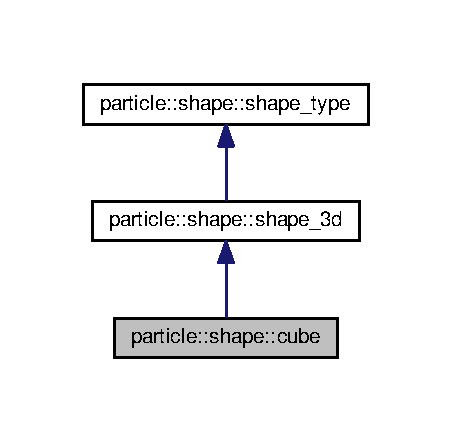
\includegraphics[width=217pt]{d6/dc4/classparticle_1_1shape_1_1cube__inherit__graph}
\end{center}
\end{figure}


Collaboration diagram for particle\+:\+:shape\+:\+:cube\+:\nopagebreak
\begin{figure}[H]
\begin{center}
\leavevmode
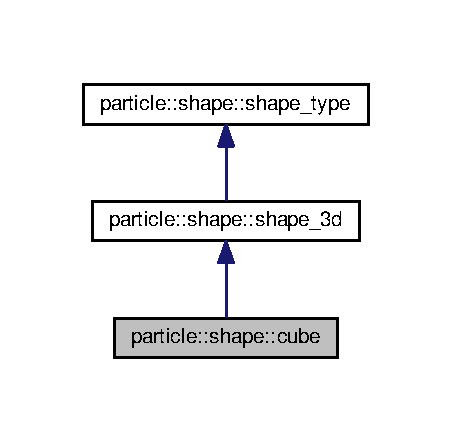
\includegraphics[width=217pt]{d9/d6b/classparticle_1_1shape_1_1cube__coll__graph}
\end{center}
\end{figure}
\subsection*{Public Member Functions}
\begin{DoxyCompactItemize}
\item 
\hyperlink{classparticle_1_1shape_1_1cube_a25e9690466125d4d09acdc79b354659c}{cube} ()
\begin{DoxyCompactList}\small\item\em Default constructor. \end{DoxyCompactList}\item 
\hyperlink{classparticle_1_1shape_1_1cube_a551fa11231e43fa349cd9b97e4f4a50e}{$\sim$cube} ()
\begin{DoxyCompactList}\small\item\em Default destructor. \end{DoxyCompactList}\end{DoxyCompactItemize}


\subsection{Detailed Description}
Cubic paritcle. 

\subsection{Constructor \& Destructor Documentation}
\index{particle\+::shape\+::cube@{particle\+::shape\+::cube}!cube@{cube}}
\index{cube@{cube}!particle\+::shape\+::cube@{particle\+::shape\+::cube}}
\subsubsection[{\texorpdfstring{cube()}{cube()}}]{\setlength{\rightskip}{0pt plus 5cm}particle\+::shape\+::cube\+::cube (
\begin{DoxyParamCaption}
{}
\end{DoxyParamCaption}
)\hspace{0.3cm}{\ttfamily [inline]}}\hypertarget{classparticle_1_1shape_1_1cube_a25e9690466125d4d09acdc79b354659c}{}\label{classparticle_1_1shape_1_1cube_a25e9690466125d4d09acdc79b354659c}


Default constructor. 

\index{particle\+::shape\+::cube@{particle\+::shape\+::cube}!````~cube@{$\sim$cube}}
\index{````~cube@{$\sim$cube}!particle\+::shape\+::cube@{particle\+::shape\+::cube}}
\subsubsection[{\texorpdfstring{$\sim$cube()}{~cube()}}]{\setlength{\rightskip}{0pt plus 5cm}particle\+::shape\+::cube\+::$\sim$cube (
\begin{DoxyParamCaption}
{}
\end{DoxyParamCaption}
)\hspace{0.3cm}{\ttfamily [inline]}}\hypertarget{classparticle_1_1shape_1_1cube_a551fa11231e43fa349cd9b97e4f4a50e}{}\label{classparticle_1_1shape_1_1cube_a551fa11231e43fa349cd9b97e4f4a50e}


Default destructor. 



The documentation for this class was generated from the following file\+:\begin{DoxyCompactItemize}
\item 
includes/\hyperlink{shape_8hpp}{shape.\+hpp}\end{DoxyCompactItemize}

\hypertarget{classparticle_1_1field_1_1field__type}{}\section{particle\+:\+:field\+:\+:field\+\_\+type Class Reference}
\label{classparticle_1_1field_1_1field__type}\index{particle\+::field\+::field\+\_\+type@{particle\+::field\+::field\+\_\+type}}


Base class for fields.  




{\ttfamily \#include $<$field\+\_\+type.\+hpp$>$}

\subsection*{Public Member Functions}
\begin{DoxyCompactItemize}
\item 
\hyperlink{classparticle_1_1field_1_1field__type_a23df5aab2db9bb195068513fdc8facab}{field\+\_\+type} ()
\begin{DoxyCompactList}\small\item\em Default constructor. \end{DoxyCompactList}\item 
\hyperlink{classparticle_1_1field_1_1field__type_a957e39bd01dddf793e324e07c8fd48b4}{field\+\_\+type} (bool ising\+\_\+in, bool periodic\+\_\+in, int d\+\_\+in, int edgesize\+\_\+in, double J\+\_\+mod, double D\+\_\+mod, std\+::string J\+\_\+filename)
\item 
\hyperlink{classparticle_1_1field_1_1field__type_abac5a921a73b94c132295ebc1840dc59}{$\sim$field\+\_\+type} ()
\begin{DoxyCompactList}\small\item\em Destructor. \end{DoxyCompactList}\item 
void \hyperlink{classparticle_1_1field_1_1field__type_a23d6de180f50944f53eb30febf7d0faf}{set\+\_\+default\+\_\+spins} ()
\begin{DoxyCompactList}\small\item\em Set default spins. \end{DoxyCompactList}\item 
xt\+::xtensorf$<$ double, xt\+::xshape$<$ 4 $>$ $>$ \& \hyperlink{classparticle_1_1field_1_1field__type_ab5c39381717c4d4b4e998edd94c99ecf}{access} (int index)
\item 
std\+::vector$<$ int $>$ \& \hyperlink{classparticle_1_1field_1_1field__type_adf78cfd03fcc91cc8d649c8ad10c28ea}{get\+\_\+neigh} (int index)
\item 
std\+::vector$<$ int $>$ \& \hyperlink{classparticle_1_1field_1_1field__type_a71b567d43943ca9a186c30cfe1abd0e4}{get\+\_\+adj} (int index)
\item 
double \& \hyperlink{classparticle_1_1field_1_1field__type_aeace7d2b757b34b941c598ce929c45a5}{get\+\_\+J} (int i, int j)
\item 
xt\+::xtensorf$<$ double, xt\+::xshape$<$ 4 $>$ $>$ \& \hyperlink{classparticle_1_1field_1_1field__type_ad722f01398113f966942bf1da7342b4b}{get\+\_\+\+D\+\_\+vec} (int i, int j)
\item 
xt\+::xtensorf$<$ int, xt\+::xshape$<$ 4 $>$ $>$ \& \hyperlink{classparticle_1_1field_1_1field__type_a3fde4fed9adefe64fa39474a7ffbf4eb}{get\+\_\+loc} (int index)
\item 
void \hyperlink{classparticle_1_1field_1_1field__type_aa200986c374b75af35f1a9a19c31861b}{add\+\_\+spin} (xt\+::xtensorf$<$ int, xt\+::xshape$<$ 4 $>$$>$ \&loc)
\item 
void \hyperlink{classparticle_1_1field_1_1field__type_a9cd7af012cad435d86a8b80be4fe7b1f}{set\+\_\+neigh} ()
\begin{DoxyCompactList}\small\item\em Determine the neighbours of the spins. \end{DoxyCompactList}\item 
unsigned int \hyperlink{classparticle_1_1field_1_1field__type_a6dfe245d4d52d1445e8088e8ba2d2149}{get\+\_\+size} ()
\item 
int \hyperlink{classparticle_1_1field_1_1field__type_aae85188d550f097c450bf8ab2f64c7f4}{get\+\_\+dim} ()
\item 
int \hyperlink{classparticle_1_1field_1_1field__type_a0668acfd198f8b8deef94d24869a20c0}{get\+\_\+edge} ()
\item 
void \hyperlink{classparticle_1_1field_1_1field__type_af58cf7684adf342fab4fc0451f876b31}{set\+\_\+rand} (int index)
\item 
void \hyperlink{classparticle_1_1field_1_1field__type_aa7afb8939edfbad8d4fdc8c2b13d2c09}{set\+\_\+up} (int index)
\item 
void \hyperlink{classparticle_1_1field_1_1field__type_a96dffd1af9e4055a1fab081ddfc3351b}{set\+\_\+down} (int index)
\item 
void \hyperlink{classparticle_1_1field_1_1field__type_aed2e6a65c7a0d4af0d5000bdb5c4df87}{set\+\_\+spin} (int index, xt\+::xtensorf$<$ double, xt\+::xshape$<$ 4 $>$ $>$ \&in)
\item 
void \hyperlink{classparticle_1_1field_1_1field__type_a3cc84c12d27dd0884235de6682647d33}{gen\+\_\+rand} ()
\begin{DoxyCompactList}\small\item\em Generate a random spin state. \end{DoxyCompactList}\item 
xt\+::xtensorf$<$ double, xt\+::xshape$<$ 4 $>$ $>$ \& \hyperlink{classparticle_1_1field_1_1field__type_ac8ea9925a2fff05c0d2fd01ff44fcc1b}{get\+\_\+rand} ()
\item 
void \hyperlink{classparticle_1_1field_1_1field__type_a3d14b4ed88a12ac2cfc0ed194ea07dc8}{all\+\_\+rand} ()
\begin{DoxyCompactList}\small\item\em Set all spins to a random state. \end{DoxyCompactList}\item 
void \hyperlink{classparticle_1_1field_1_1field__type_a0ea5e47a876e032d71f80f36fb7d420e}{all\+\_\+zero} ()
\begin{DoxyCompactList}\small\item\em Set all spins to a zero state. \end{DoxyCompactList}\item 
void \hyperlink{classparticle_1_1field_1_1field__type_affdbf54dbaf99790a4002c0a34a41617}{print} (std\+::string filename, std\+::string arrname)
\item 
void \hyperlink{classparticle_1_1field_1_1field__type_a556f4573caf7bbf30a5319e8b7d72135}{send\+\_\+data} (int dest\+\_\+rank)
\item 
void \hyperlink{classparticle_1_1field_1_1field__type_aca156c7b050285ed49e941961059dedb}{recv\+\_\+data} (int src\+\_\+rank)
\item 
bool \hyperlink{classparticle_1_1field_1_1field__type_a5563deee195c3191007c0a139e2f389e}{use\+\_\+J} ()
\begin{DoxyCompactList}\small\item\em Are the exchanges on? \end{DoxyCompactList}\item 
bool \hyperlink{classparticle_1_1field_1_1field__type_a22b27d6b2ce32ea93ed5113a513f0f16}{use\+\_\+D} ()
\begin{DoxyCompactList}\small\item\em Are the dmis on? \end{DoxyCompactList}\end{DoxyCompactItemize}


\subsection{Detailed Description}
Base class for fields. 

\subsection{Constructor \& Destructor Documentation}
\index{particle\+::field\+::field\+\_\+type@{particle\+::field\+::field\+\_\+type}!field\+\_\+type@{field\+\_\+type}}
\index{field\+\_\+type@{field\+\_\+type}!particle\+::field\+::field\+\_\+type@{particle\+::field\+::field\+\_\+type}}
\subsubsection[{\texorpdfstring{field\+\_\+type()}{field_type()}}]{\setlength{\rightskip}{0pt plus 5cm}particle\+::field\+::field\+\_\+type\+::field\+\_\+type (
\begin{DoxyParamCaption}
{}
\end{DoxyParamCaption}
)\hspace{0.3cm}{\ttfamily [inline]}}\hypertarget{classparticle_1_1field_1_1field__type_a23df5aab2db9bb195068513fdc8facab}{}\label{classparticle_1_1field_1_1field__type_a23df5aab2db9bb195068513fdc8facab}


Default constructor. 

\index{particle\+::field\+::field\+\_\+type@{particle\+::field\+::field\+\_\+type}!field\+\_\+type@{field\+\_\+type}}
\index{field\+\_\+type@{field\+\_\+type}!particle\+::field\+::field\+\_\+type@{particle\+::field\+::field\+\_\+type}}
\subsubsection[{\texorpdfstring{field\+\_\+type(bool ising\+\_\+in, bool periodic\+\_\+in, int d\+\_\+in, int edgesize\+\_\+in, double J\+\_\+mod, double D\+\_\+mod, std\+::string J\+\_\+filename)}{field_type(bool ising_in, bool periodic_in, int d_in, int edgesize_in, double J_mod, double D_mod, std::string J_filename)}}]{\setlength{\rightskip}{0pt plus 5cm}particle\+::field\+::field\+\_\+type\+::field\+\_\+type (
\begin{DoxyParamCaption}
\item[{bool}]{ising\+\_\+in, }
\item[{bool}]{periodic\+\_\+in, }
\item[{int}]{d\+\_\+in, }
\item[{int}]{edgesize\+\_\+in, }
\item[{double}]{J\+\_\+mod, }
\item[{double}]{D\+\_\+mod, }
\item[{std\+::string}]{J\+\_\+filename}
\end{DoxyParamCaption}
)}\hypertarget{classparticle_1_1field_1_1field__type_a957e39bd01dddf793e324e07c8fd48b4}{}\label{classparticle_1_1field_1_1field__type_a957e39bd01dddf793e324e07c8fd48b4}
Constructor


\begin{DoxyParams}{Parameters}
{\em ising\+\_\+in} & Is this an ising field? \\
\hline
{\em periodic\+\_\+in} & Is the field periodic? \\
\hline
{\em d\+\_\+in} & The dimension of the field \\
\hline
{\em edgesize\+\_\+in} & The edgelength of the lattice \\
\hline
{\em J\+\_\+mod} & A modifier for the strength of the exchange \\
\hline
{\em D\+\_\+mod} & A modifier for the strength of the D\+MI \\
\hline
{\em J\+\_\+filename} & The filename where the exchanges and D\+M\+Is are stored \\
\hline
\end{DoxyParams}
\index{particle\+::field\+::field\+\_\+type@{particle\+::field\+::field\+\_\+type}!````~field\+\_\+type@{$\sim$field\+\_\+type}}
\index{````~field\+\_\+type@{$\sim$field\+\_\+type}!particle\+::field\+::field\+\_\+type@{particle\+::field\+::field\+\_\+type}}
\subsubsection[{\texorpdfstring{$\sim$field\+\_\+type()}{~field_type()}}]{\setlength{\rightskip}{0pt plus 5cm}particle\+::field\+::field\+\_\+type\+::$\sim$field\+\_\+type (
\begin{DoxyParamCaption}
{}
\end{DoxyParamCaption}
)\hspace{0.3cm}{\ttfamily [inline]}}\hypertarget{classparticle_1_1field_1_1field__type_abac5a921a73b94c132295ebc1840dc59}{}\label{classparticle_1_1field_1_1field__type_abac5a921a73b94c132295ebc1840dc59}


Destructor. 



\subsection{Member Function Documentation}
\index{particle\+::field\+::field\+\_\+type@{particle\+::field\+::field\+\_\+type}!access@{access}}
\index{access@{access}!particle\+::field\+::field\+\_\+type@{particle\+::field\+::field\+\_\+type}}
\subsubsection[{\texorpdfstring{access(int index)}{access(int index)}}]{\setlength{\rightskip}{0pt plus 5cm}xt\+::xtensorf$<$double, xt\+::xshape$<$4$>$ $>$\& particle\+::field\+::field\+\_\+type\+::access (
\begin{DoxyParamCaption}
\item[{int}]{index}
\end{DoxyParamCaption}
)\hspace{0.3cm}{\ttfamily [inline]}}\hypertarget{classparticle_1_1field_1_1field__type_ab5c39381717c4d4b4e998edd94c99ecf}{}\label{classparticle_1_1field_1_1field__type_ab5c39381717c4d4b4e998edd94c99ecf}
Access an individual spin


\begin{DoxyParams}{Parameters}
{\em index} & The index of the spin site \\
\hline
\end{DoxyParams}
\begin{DoxyReturn}{Returns}
A reference to the spin value as a valarray 
\end{DoxyReturn}
\index{particle\+::field\+::field\+\_\+type@{particle\+::field\+::field\+\_\+type}!add\+\_\+spin@{add\+\_\+spin}}
\index{add\+\_\+spin@{add\+\_\+spin}!particle\+::field\+::field\+\_\+type@{particle\+::field\+::field\+\_\+type}}
\subsubsection[{\texorpdfstring{add\+\_\+spin(xt\+::xtensorf$<$ int, xt\+::xshape$<$ 4 $>$$>$ \&loc)}{add_spin(xt::xtensorf< int, xt::xshape< 4 >> &loc)}}]{\setlength{\rightskip}{0pt plus 5cm}void particle\+::field\+::field\+\_\+type\+::add\+\_\+spin (
\begin{DoxyParamCaption}
\item[{xt\+::xtensorf$<$ int, xt\+::xshape$<$ 4 $>$$>$ \&}]{loc}
\end{DoxyParamCaption}
)}\hypertarget{classparticle_1_1field_1_1field__type_aa200986c374b75af35f1a9a19c31861b}{}\label{classparticle_1_1field_1_1field__type_aa200986c374b75af35f1a9a19c31861b}
Add a new spin to the field of spins


\begin{DoxyParams}{Parameters}
{\em loc} & The location of the new spin \\
\hline
\end{DoxyParams}
\index{particle\+::field\+::field\+\_\+type@{particle\+::field\+::field\+\_\+type}!all\+\_\+rand@{all\+\_\+rand}}
\index{all\+\_\+rand@{all\+\_\+rand}!particle\+::field\+::field\+\_\+type@{particle\+::field\+::field\+\_\+type}}
\subsubsection[{\texorpdfstring{all\+\_\+rand()}{all_rand()}}]{\setlength{\rightskip}{0pt plus 5cm}void particle\+::field\+::field\+\_\+type\+::all\+\_\+rand (
\begin{DoxyParamCaption}
{}
\end{DoxyParamCaption}
)}\hypertarget{classparticle_1_1field_1_1field__type_a3d14b4ed88a12ac2cfc0ed194ea07dc8}{}\label{classparticle_1_1field_1_1field__type_a3d14b4ed88a12ac2cfc0ed194ea07dc8}


Set all spins to a random state. 

\index{particle\+::field\+::field\+\_\+type@{particle\+::field\+::field\+\_\+type}!all\+\_\+zero@{all\+\_\+zero}}
\index{all\+\_\+zero@{all\+\_\+zero}!particle\+::field\+::field\+\_\+type@{particle\+::field\+::field\+\_\+type}}
\subsubsection[{\texorpdfstring{all\+\_\+zero()}{all_zero()}}]{\setlength{\rightskip}{0pt plus 5cm}void particle\+::field\+::field\+\_\+type\+::all\+\_\+zero (
\begin{DoxyParamCaption}
{}
\end{DoxyParamCaption}
)}\hypertarget{classparticle_1_1field_1_1field__type_a0ea5e47a876e032d71f80f36fb7d420e}{}\label{classparticle_1_1field_1_1field__type_a0ea5e47a876e032d71f80f36fb7d420e}


Set all spins to a zero state. 

\index{particle\+::field\+::field\+\_\+type@{particle\+::field\+::field\+\_\+type}!gen\+\_\+rand@{gen\+\_\+rand}}
\index{gen\+\_\+rand@{gen\+\_\+rand}!particle\+::field\+::field\+\_\+type@{particle\+::field\+::field\+\_\+type}}
\subsubsection[{\texorpdfstring{gen\+\_\+rand()}{gen_rand()}}]{\setlength{\rightskip}{0pt plus 5cm}void particle\+::field\+::field\+\_\+type\+::gen\+\_\+rand (
\begin{DoxyParamCaption}
{}
\end{DoxyParamCaption}
)}\hypertarget{classparticle_1_1field_1_1field__type_a3cc84c12d27dd0884235de6682647d33}{}\label{classparticle_1_1field_1_1field__type_a3cc84c12d27dd0884235de6682647d33}


Generate a random spin state. 

\index{particle\+::field\+::field\+\_\+type@{particle\+::field\+::field\+\_\+type}!get\+\_\+adj@{get\+\_\+adj}}
\index{get\+\_\+adj@{get\+\_\+adj}!particle\+::field\+::field\+\_\+type@{particle\+::field\+::field\+\_\+type}}
\subsubsection[{\texorpdfstring{get\+\_\+adj(int index)}{get_adj(int index)}}]{\setlength{\rightskip}{0pt plus 5cm}std\+::vector$<$int$>$\& particle\+::field\+::field\+\_\+type\+::get\+\_\+adj (
\begin{DoxyParamCaption}
\item[{int}]{index}
\end{DoxyParamCaption}
)\hspace{0.3cm}{\ttfamily [inline]}}\hypertarget{classparticle_1_1field_1_1field__type_a71b567d43943ca9a186c30cfe1abd0e4}{}\label{classparticle_1_1field_1_1field__type_a71b567d43943ca9a186c30cfe1abd0e4}
Get the neighbours of a spin site


\begin{DoxyParams}{Parameters}
{\em index} & The index of the spin site \\
\hline
\end{DoxyParams}
\begin{DoxyReturn}{Returns}
A vector containing the indices of the neighbours of the chosen spin 
\end{DoxyReturn}
\index{particle\+::field\+::field\+\_\+type@{particle\+::field\+::field\+\_\+type}!get\+\_\+\+D\+\_\+vec@{get\+\_\+\+D\+\_\+vec}}
\index{get\+\_\+\+D\+\_\+vec@{get\+\_\+\+D\+\_\+vec}!particle\+::field\+::field\+\_\+type@{particle\+::field\+::field\+\_\+type}}
\subsubsection[{\texorpdfstring{get\+\_\+\+D\+\_\+vec(int i, int j)}{get_D_vec(int i, int j)}}]{\setlength{\rightskip}{0pt plus 5cm}xt\+::xtensorf$<$double, xt\+::xshape$<$4$>$ $>$\& particle\+::field\+::field\+\_\+type\+::get\+\_\+\+D\+\_\+vec (
\begin{DoxyParamCaption}
\item[{int}]{i, }
\item[{int}]{j}
\end{DoxyParamCaption}
)\hspace{0.3cm}{\ttfamily [inline]}}\hypertarget{classparticle_1_1field_1_1field__type_ad722f01398113f966942bf1da7342b4b}{}\label{classparticle_1_1field_1_1field__type_ad722f01398113f966942bf1da7342b4b}
Get the D\+MI vector with the neighbours of a spin site


\begin{DoxyParams}{Parameters}
{\em i} & The index of the spin site \\
\hline
{\em j} & The index of the chosen neighbour \\
\hline
\end{DoxyParams}
\begin{DoxyReturn}{Returns}
The D\+MI vector between the two spins 
\end{DoxyReturn}
\index{particle\+::field\+::field\+\_\+type@{particle\+::field\+::field\+\_\+type}!get\+\_\+dim@{get\+\_\+dim}}
\index{get\+\_\+dim@{get\+\_\+dim}!particle\+::field\+::field\+\_\+type@{particle\+::field\+::field\+\_\+type}}
\subsubsection[{\texorpdfstring{get\+\_\+dim()}{get_dim()}}]{\setlength{\rightskip}{0pt plus 5cm}int particle\+::field\+::field\+\_\+type\+::get\+\_\+dim (
\begin{DoxyParamCaption}
{}
\end{DoxyParamCaption}
)\hspace{0.3cm}{\ttfamily [inline]}}\hypertarget{classparticle_1_1field_1_1field__type_aae85188d550f097c450bf8ab2f64c7f4}{}\label{classparticle_1_1field_1_1field__type_aae85188d550f097c450bf8ab2f64c7f4}
Get the dimension in the field

\begin{DoxyReturn}{Returns}
The dimension of the field 
\end{DoxyReturn}
\index{particle\+::field\+::field\+\_\+type@{particle\+::field\+::field\+\_\+type}!get\+\_\+edge@{get\+\_\+edge}}
\index{get\+\_\+edge@{get\+\_\+edge}!particle\+::field\+::field\+\_\+type@{particle\+::field\+::field\+\_\+type}}
\subsubsection[{\texorpdfstring{get\+\_\+edge()}{get_edge()}}]{\setlength{\rightskip}{0pt plus 5cm}int particle\+::field\+::field\+\_\+type\+::get\+\_\+edge (
\begin{DoxyParamCaption}
{}
\end{DoxyParamCaption}
)\hspace{0.3cm}{\ttfamily [inline]}}\hypertarget{classparticle_1_1field_1_1field__type_a0668acfd198f8b8deef94d24869a20c0}{}\label{classparticle_1_1field_1_1field__type_a0668acfd198f8b8deef94d24869a20c0}
Get the edgesize of the field

\begin{DoxyReturn}{Returns}
The edgesize of the field 
\end{DoxyReturn}
\index{particle\+::field\+::field\+\_\+type@{particle\+::field\+::field\+\_\+type}!get\+\_\+J@{get\+\_\+J}}
\index{get\+\_\+J@{get\+\_\+J}!particle\+::field\+::field\+\_\+type@{particle\+::field\+::field\+\_\+type}}
\subsubsection[{\texorpdfstring{get\+\_\+\+J(int i, int j)}{get_J(int i, int j)}}]{\setlength{\rightskip}{0pt plus 5cm}double\& particle\+::field\+::field\+\_\+type\+::get\+\_\+J (
\begin{DoxyParamCaption}
\item[{int}]{i, }
\item[{int}]{j}
\end{DoxyParamCaption}
)\hspace{0.3cm}{\ttfamily [inline]}}\hypertarget{classparticle_1_1field_1_1field__type_aeace7d2b757b34b941c598ce929c45a5}{}\label{classparticle_1_1field_1_1field__type_aeace7d2b757b34b941c598ce929c45a5}
Get the exchanges with the neighbours of a spin site


\begin{DoxyParams}{Parameters}
{\em i} & The index of the spin site \\
\hline
{\em j} & The index of the chosen neighbour \\
\hline
\end{DoxyParams}
\begin{DoxyReturn}{Returns}
The exchange between the two spins 
\end{DoxyReturn}
\index{particle\+::field\+::field\+\_\+type@{particle\+::field\+::field\+\_\+type}!get\+\_\+loc@{get\+\_\+loc}}
\index{get\+\_\+loc@{get\+\_\+loc}!particle\+::field\+::field\+\_\+type@{particle\+::field\+::field\+\_\+type}}
\subsubsection[{\texorpdfstring{get\+\_\+loc(int index)}{get_loc(int index)}}]{\setlength{\rightskip}{0pt plus 5cm}xt\+::xtensorf$<$int, xt\+::xshape$<$4$>$ $>$\& particle\+::field\+::field\+\_\+type\+::get\+\_\+loc (
\begin{DoxyParamCaption}
\item[{int}]{index}
\end{DoxyParamCaption}
)\hspace{0.3cm}{\ttfamily [inline]}}\hypertarget{classparticle_1_1field_1_1field__type_a3fde4fed9adefe64fa39474a7ffbf4eb}{}\label{classparticle_1_1field_1_1field__type_a3fde4fed9adefe64fa39474a7ffbf4eb}
Get the location of a spin site


\begin{DoxyParams}{Parameters}
{\em index} & The index of the spin site \\
\hline
\end{DoxyParams}
\begin{DoxyReturn}{Returns}
A vector containing the location of the neighbours of the chosen spin 
\end{DoxyReturn}
\index{particle\+::field\+::field\+\_\+type@{particle\+::field\+::field\+\_\+type}!get\+\_\+neigh@{get\+\_\+neigh}}
\index{get\+\_\+neigh@{get\+\_\+neigh}!particle\+::field\+::field\+\_\+type@{particle\+::field\+::field\+\_\+type}}
\subsubsection[{\texorpdfstring{get\+\_\+neigh(int index)}{get_neigh(int index)}}]{\setlength{\rightskip}{0pt plus 5cm}std\+::vector$<$int$>$\& particle\+::field\+::field\+\_\+type\+::get\+\_\+neigh (
\begin{DoxyParamCaption}
\item[{int}]{index}
\end{DoxyParamCaption}
)\hspace{0.3cm}{\ttfamily [inline]}}\hypertarget{classparticle_1_1field_1_1field__type_adf78cfd03fcc91cc8d649c8ad10c28ea}{}\label{classparticle_1_1field_1_1field__type_adf78cfd03fcc91cc8d649c8ad10c28ea}
Get the neighbours of a spin site


\begin{DoxyParams}{Parameters}
{\em index} & The index of the spin site \\
\hline
\end{DoxyParams}
\begin{DoxyReturn}{Returns}
A vector containing the indices of the neighbours of the chosen spin 
\end{DoxyReturn}
\index{particle\+::field\+::field\+\_\+type@{particle\+::field\+::field\+\_\+type}!get\+\_\+rand@{get\+\_\+rand}}
\index{get\+\_\+rand@{get\+\_\+rand}!particle\+::field\+::field\+\_\+type@{particle\+::field\+::field\+\_\+type}}
\subsubsection[{\texorpdfstring{get\+\_\+rand()}{get_rand()}}]{\setlength{\rightskip}{0pt plus 5cm}xt\+::xtensorf$<$double, xt\+::xshape$<$4$>$ $>$\& particle\+::field\+::field\+\_\+type\+::get\+\_\+rand (
\begin{DoxyParamCaption}
{}
\end{DoxyParamCaption}
)\hspace{0.3cm}{\ttfamily [inline]}}\hypertarget{classparticle_1_1field_1_1field__type_ac8ea9925a2fff05c0d2fd01ff44fcc1b}{}\label{classparticle_1_1field_1_1field__type_ac8ea9925a2fff05c0d2fd01ff44fcc1b}
Return the randomly generated state

\begin{DoxyReturn}{Returns}
The random state as a valarray 
\end{DoxyReturn}
\index{particle\+::field\+::field\+\_\+type@{particle\+::field\+::field\+\_\+type}!get\+\_\+size@{get\+\_\+size}}
\index{get\+\_\+size@{get\+\_\+size}!particle\+::field\+::field\+\_\+type@{particle\+::field\+::field\+\_\+type}}
\subsubsection[{\texorpdfstring{get\+\_\+size()}{get_size()}}]{\setlength{\rightskip}{0pt plus 5cm}unsigned int particle\+::field\+::field\+\_\+type\+::get\+\_\+size (
\begin{DoxyParamCaption}
{}
\end{DoxyParamCaption}
)\hspace{0.3cm}{\ttfamily [inline]}}\hypertarget{classparticle_1_1field_1_1field__type_a6dfe245d4d52d1445e8088e8ba2d2149}{}\label{classparticle_1_1field_1_1field__type_a6dfe245d4d52d1445e8088e8ba2d2149}
Get the number of spins in the field

\begin{DoxyReturn}{Returns}
The number of spins in the field 
\end{DoxyReturn}
\index{particle\+::field\+::field\+\_\+type@{particle\+::field\+::field\+\_\+type}!print@{print}}
\index{print@{print}!particle\+::field\+::field\+\_\+type@{particle\+::field\+::field\+\_\+type}}
\subsubsection[{\texorpdfstring{print(std\+::string filename, std\+::string arrname)}{print(std::string filename, std::string arrname)}}]{\setlength{\rightskip}{0pt plus 5cm}void particle\+::field\+::field\+\_\+type\+::print (
\begin{DoxyParamCaption}
\item[{std\+::string}]{filename, }
\item[{std\+::string}]{arrname}
\end{DoxyParamCaption}
)}\hypertarget{classparticle_1_1field_1_1field__type_affdbf54dbaf99790a4002c0a34a41617}{}\label{classparticle_1_1field_1_1field__type_affdbf54dbaf99790a4002c0a34a41617}
Print the lattice to a file

/param filename The name of the H\+D\+F5 file /param arrname The name of the particular array to be printed to \index{particle\+::field\+::field\+\_\+type@{particle\+::field\+::field\+\_\+type}!recv\+\_\+data@{recv\+\_\+data}}
\index{recv\+\_\+data@{recv\+\_\+data}!particle\+::field\+::field\+\_\+type@{particle\+::field\+::field\+\_\+type}}
\subsubsection[{\texorpdfstring{recv\+\_\+data(int src\+\_\+rank)}{recv_data(int src_rank)}}]{\setlength{\rightskip}{0pt plus 5cm}void particle\+::field\+::field\+\_\+type\+::recv\+\_\+data (
\begin{DoxyParamCaption}
\item[{int}]{src\+\_\+rank}
\end{DoxyParamCaption}
)}\hypertarget{classparticle_1_1field_1_1field__type_aca156c7b050285ed49e941961059dedb}{}\label{classparticle_1_1field_1_1field__type_aca156c7b050285ed49e941961059dedb}
Recieve the field from another process


\begin{DoxyParams}{Parameters}
{\em src\+\_\+rank} & The rank of the process recieving from \\
\hline
\end{DoxyParams}
\index{particle\+::field\+::field\+\_\+type@{particle\+::field\+::field\+\_\+type}!send\+\_\+data@{send\+\_\+data}}
\index{send\+\_\+data@{send\+\_\+data}!particle\+::field\+::field\+\_\+type@{particle\+::field\+::field\+\_\+type}}
\subsubsection[{\texorpdfstring{send\+\_\+data(int dest\+\_\+rank)}{send_data(int dest_rank)}}]{\setlength{\rightskip}{0pt plus 5cm}void particle\+::field\+::field\+\_\+type\+::send\+\_\+data (
\begin{DoxyParamCaption}
\item[{int}]{dest\+\_\+rank}
\end{DoxyParamCaption}
)}\hypertarget{classparticle_1_1field_1_1field__type_a556f4573caf7bbf30a5319e8b7d72135}{}\label{classparticle_1_1field_1_1field__type_a556f4573caf7bbf30a5319e8b7d72135}
Send the field to another process


\begin{DoxyParams}{Parameters}
{\em dest\+\_\+rank} & The target process\textquotesingle{} rank \\
\hline
\end{DoxyParams}
\index{particle\+::field\+::field\+\_\+type@{particle\+::field\+::field\+\_\+type}!set\+\_\+default\+\_\+spins@{set\+\_\+default\+\_\+spins}}
\index{set\+\_\+default\+\_\+spins@{set\+\_\+default\+\_\+spins}!particle\+::field\+::field\+\_\+type@{particle\+::field\+::field\+\_\+type}}
\subsubsection[{\texorpdfstring{set\+\_\+default\+\_\+spins()}{set_default_spins()}}]{\setlength{\rightskip}{0pt plus 5cm}void particle\+::field\+::field\+\_\+type\+::set\+\_\+default\+\_\+spins (
\begin{DoxyParamCaption}
{}
\end{DoxyParamCaption}
)}\hypertarget{classparticle_1_1field_1_1field__type_a23d6de180f50944f53eb30febf7d0faf}{}\label{classparticle_1_1field_1_1field__type_a23d6de180f50944f53eb30febf7d0faf}


Set default spins. 

\index{particle\+::field\+::field\+\_\+type@{particle\+::field\+::field\+\_\+type}!set\+\_\+down@{set\+\_\+down}}
\index{set\+\_\+down@{set\+\_\+down}!particle\+::field\+::field\+\_\+type@{particle\+::field\+::field\+\_\+type}}
\subsubsection[{\texorpdfstring{set\+\_\+down(int index)}{set_down(int index)}}]{\setlength{\rightskip}{0pt plus 5cm}void particle\+::field\+::field\+\_\+type\+::set\+\_\+down (
\begin{DoxyParamCaption}
\item[{int}]{index}
\end{DoxyParamCaption}
)\hspace{0.3cm}{\ttfamily [inline]}}\hypertarget{classparticle_1_1field_1_1field__type_a96dffd1af9e4055a1fab081ddfc3351b}{}\label{classparticle_1_1field_1_1field__type_a96dffd1af9e4055a1fab081ddfc3351b}
Set a spin to the down state


\begin{DoxyParams}{Parameters}
{\em index} & The location of the spin to be changed \\
\hline
\end{DoxyParams}
\index{particle\+::field\+::field\+\_\+type@{particle\+::field\+::field\+\_\+type}!set\+\_\+neigh@{set\+\_\+neigh}}
\index{set\+\_\+neigh@{set\+\_\+neigh}!particle\+::field\+::field\+\_\+type@{particle\+::field\+::field\+\_\+type}}
\subsubsection[{\texorpdfstring{set\+\_\+neigh()}{set_neigh()}}]{\setlength{\rightskip}{0pt plus 5cm}void particle\+::field\+::field\+\_\+type\+::set\+\_\+neigh (
\begin{DoxyParamCaption}
{}
\end{DoxyParamCaption}
)}\hypertarget{classparticle_1_1field_1_1field__type_a9cd7af012cad435d86a8b80be4fe7b1f}{}\label{classparticle_1_1field_1_1field__type_a9cd7af012cad435d86a8b80be4fe7b1f}


Determine the neighbours of the spins. 

\index{particle\+::field\+::field\+\_\+type@{particle\+::field\+::field\+\_\+type}!set\+\_\+rand@{set\+\_\+rand}}
\index{set\+\_\+rand@{set\+\_\+rand}!particle\+::field\+::field\+\_\+type@{particle\+::field\+::field\+\_\+type}}
\subsubsection[{\texorpdfstring{set\+\_\+rand(int index)}{set_rand(int index)}}]{\setlength{\rightskip}{0pt plus 5cm}void particle\+::field\+::field\+\_\+type\+::set\+\_\+rand (
\begin{DoxyParamCaption}
\item[{int}]{index}
\end{DoxyParamCaption}
)\hspace{0.3cm}{\ttfamily [inline]}}\hypertarget{classparticle_1_1field_1_1field__type_af58cf7684adf342fab4fc0451f876b31}{}\label{classparticle_1_1field_1_1field__type_af58cf7684adf342fab4fc0451f876b31}
Set a spin to the already generated random state


\begin{DoxyParams}{Parameters}
{\em index} & The location of the spin to be changed \\
\hline
\end{DoxyParams}
\index{particle\+::field\+::field\+\_\+type@{particle\+::field\+::field\+\_\+type}!set\+\_\+spin@{set\+\_\+spin}}
\index{set\+\_\+spin@{set\+\_\+spin}!particle\+::field\+::field\+\_\+type@{particle\+::field\+::field\+\_\+type}}
\subsubsection[{\texorpdfstring{set\+\_\+spin(int index, xt\+::xtensorf$<$ double, xt\+::xshape$<$ 4 $>$ $>$ \&in)}{set_spin(int index, xt::xtensorf< double, xt::xshape< 4 > > &in)}}]{\setlength{\rightskip}{0pt plus 5cm}void particle\+::field\+::field\+\_\+type\+::set\+\_\+spin (
\begin{DoxyParamCaption}
\item[{int}]{index, }
\item[{xt\+::xtensorf$<$ double, xt\+::xshape$<$ 4 $>$ $>$ \&}]{in}
\end{DoxyParamCaption}
)\hspace{0.3cm}{\ttfamily [inline]}}\hypertarget{classparticle_1_1field_1_1field__type_aed2e6a65c7a0d4af0d5000bdb5c4df87}{}\label{classparticle_1_1field_1_1field__type_aed2e6a65c7a0d4af0d5000bdb5c4df87}
Set a spin to the down state


\begin{DoxyParams}{Parameters}
{\em index} & The location of the spin to be changed \\
\hline
\end{DoxyParams}
\index{particle\+::field\+::field\+\_\+type@{particle\+::field\+::field\+\_\+type}!set\+\_\+up@{set\+\_\+up}}
\index{set\+\_\+up@{set\+\_\+up}!particle\+::field\+::field\+\_\+type@{particle\+::field\+::field\+\_\+type}}
\subsubsection[{\texorpdfstring{set\+\_\+up(int index)}{set_up(int index)}}]{\setlength{\rightskip}{0pt plus 5cm}void particle\+::field\+::field\+\_\+type\+::set\+\_\+up (
\begin{DoxyParamCaption}
\item[{int}]{index}
\end{DoxyParamCaption}
)\hspace{0.3cm}{\ttfamily [inline]}}\hypertarget{classparticle_1_1field_1_1field__type_aa7afb8939edfbad8d4fdc8c2b13d2c09}{}\label{classparticle_1_1field_1_1field__type_aa7afb8939edfbad8d4fdc8c2b13d2c09}
Set a spin to the down state


\begin{DoxyParams}{Parameters}
{\em index} & The location of the spin to be changed \\
\hline
\end{DoxyParams}
\index{particle\+::field\+::field\+\_\+type@{particle\+::field\+::field\+\_\+type}!use\+\_\+D@{use\+\_\+D}}
\index{use\+\_\+D@{use\+\_\+D}!particle\+::field\+::field\+\_\+type@{particle\+::field\+::field\+\_\+type}}
\subsubsection[{\texorpdfstring{use\+\_\+\+D()}{use_D()}}]{\setlength{\rightskip}{0pt plus 5cm}bool particle\+::field\+::field\+\_\+type\+::use\+\_\+D (
\begin{DoxyParamCaption}
{}
\end{DoxyParamCaption}
)\hspace{0.3cm}{\ttfamily [inline]}}\hypertarget{classparticle_1_1field_1_1field__type_a22b27d6b2ce32ea93ed5113a513f0f16}{}\label{classparticle_1_1field_1_1field__type_a22b27d6b2ce32ea93ed5113a513f0f16}


Are the dmis on? 

\index{particle\+::field\+::field\+\_\+type@{particle\+::field\+::field\+\_\+type}!use\+\_\+J@{use\+\_\+J}}
\index{use\+\_\+J@{use\+\_\+J}!particle\+::field\+::field\+\_\+type@{particle\+::field\+::field\+\_\+type}}
\subsubsection[{\texorpdfstring{use\+\_\+\+J()}{use_J()}}]{\setlength{\rightskip}{0pt plus 5cm}bool particle\+::field\+::field\+\_\+type\+::use\+\_\+J (
\begin{DoxyParamCaption}
{}
\end{DoxyParamCaption}
)\hspace{0.3cm}{\ttfamily [inline]}}\hypertarget{classparticle_1_1field_1_1field__type_a5563deee195c3191007c0a139e2f389e}{}\label{classparticle_1_1field_1_1field__type_a5563deee195c3191007c0a139e2f389e}


Are the exchanges on? 



The documentation for this class was generated from the following file\+:\begin{DoxyCompactItemize}
\item 
includes/\hyperlink{field__type_8hpp}{field\+\_\+type.\+hpp}\end{DoxyCompactItemize}

\hypertarget{classparticle_1_1td_1_1functionObject}{}\section{particle\+:\+:td\+:\+:function\+Object Class Reference}
\label{classparticle_1_1td_1_1functionObject}\index{particle\+::td\+::function\+Object@{particle\+::td\+::function\+Object}}


{\ttfamily \#include $<$thermodynamics.\+hpp$>$}

\subsection*{Public Member Functions}
\begin{DoxyCompactItemize}
\item 
void \hyperlink{classparticle_1_1td_1_1functionObject_a983e51c31ec252ab0567eb70bc0a8631}{setup} (bool useJ, bool useD)
\item 
double \hyperlink{classparticle_1_1td_1_1functionObject_a7fe36af330daf78dbe7ce3897e6dad3f}{calc\+\_\+E} (\hyperlink{classparticle_1_1field_1_1field__type}{field\+::field\+\_\+type} \&lattice, xt\+::xtensorf$<$ double, xt\+::xshape$<$ 4 $>$$>$ \&H)
\item 
double \hyperlink{classparticle_1_1td_1_1functionObject_a057b7d5d3315a6a36efa470d4136ceb7}{calc\+\_\+dE} (\hyperlink{classparticle_1_1field_1_1field__type}{field\+::field\+\_\+type} \&lattice, int position, xt\+::xtensorf$<$ double, xt\+::xshape$<$ 4 $>$$>$ \&H)
\item 
xt\+::xtensorf$<$ double, xt\+::xshape$<$ 4 $>$ $>$ \hyperlink{classparticle_1_1td_1_1functionObject_a60a3f8d3dc9160864d6c05bc4583b8b7}{calc\+\_\+M} (\hyperlink{classparticle_1_1field_1_1field__type}{field\+::field\+\_\+type} \&lattice)
\item 
xt\+::xtensorf$<$ double, xt\+::xshape$<$ 4 $>$ $>$ \hyperlink{classparticle_1_1td_1_1functionObject_a1b92821d8ef6d7aee3d0baeaeef6db1f}{calc\+\_\+subM} (\hyperlink{classparticle_1_1field_1_1field__type}{field\+::field\+\_\+type} \&lattice, int subnumber)
\item 
std\+::vector$<$ double $>$ \hyperlink{classparticle_1_1td_1_1functionObject_aef4fdc9fa9647aa342978820c2c9a4fc}{calc\+\_\+\+TC} (\hyperlink{classparticle_1_1field_1_1field__type}{field\+::field\+\_\+type} \&lattice)
\end{DoxyCompactItemize}


\subsection{Member Function Documentation}
\index{particle\+::td\+::function\+Object@{particle\+::td\+::function\+Object}!calc\+\_\+dE@{calc\+\_\+dE}}
\index{calc\+\_\+dE@{calc\+\_\+dE}!particle\+::td\+::function\+Object@{particle\+::td\+::function\+Object}}
\subsubsection[{\texorpdfstring{calc\+\_\+d\+E(field\+::field\+\_\+type \&lattice, int position, xt\+::xtensorf$<$ double, xt\+::xshape$<$ 4 $>$$>$ \&\+H)}{calc_dE(field::field_type &lattice, int position, xt::xtensorf< double, xt::xshape< 4 >> &H)}}]{\setlength{\rightskip}{0pt plus 5cm}double particle\+::td\+::function\+Object\+::calc\+\_\+dE (
\begin{DoxyParamCaption}
\item[{{\bf field\+::field\+\_\+type} \&}]{lattice, }
\item[{int}]{position, }
\item[{xt\+::xtensorf$<$ double, xt\+::xshape$<$ 4 $>$$>$ \&}]{H}
\end{DoxyParamCaption}
)\hspace{0.3cm}{\ttfamily [inline]}}\hypertarget{classparticle_1_1td_1_1functionObject_a057b7d5d3315a6a36efa470d4136ceb7}{}\label{classparticle_1_1td_1_1functionObject_a057b7d5d3315a6a36efa470d4136ceb7}
Calculate the energy change after a spin flip of a single spin


\begin{DoxyParams}{Parameters}
{\em lattice} & The lattice \\
\hline
{\em position} & The chosen spin \\
\hline
{\em H} & The external magnetic field \\
\hline
\end{DoxyParams}
\begin{DoxyReturn}{Returns}
The change in energy 
\end{DoxyReturn}
\index{particle\+::td\+::function\+Object@{particle\+::td\+::function\+Object}!calc\+\_\+E@{calc\+\_\+E}}
\index{calc\+\_\+E@{calc\+\_\+E}!particle\+::td\+::function\+Object@{particle\+::td\+::function\+Object}}
\subsubsection[{\texorpdfstring{calc\+\_\+\+E(field\+::field\+\_\+type \&lattice, xt\+::xtensorf$<$ double, xt\+::xshape$<$ 4 $>$$>$ \&\+H)}{calc_E(field::field_type &lattice, xt::xtensorf< double, xt::xshape< 4 >> &H)}}]{\setlength{\rightskip}{0pt plus 5cm}double particle\+::td\+::function\+Object\+::calc\+\_\+E (
\begin{DoxyParamCaption}
\item[{{\bf field\+::field\+\_\+type} \&}]{lattice, }
\item[{xt\+::xtensorf$<$ double, xt\+::xshape$<$ 4 $>$$>$ \&}]{H}
\end{DoxyParamCaption}
)\hspace{0.3cm}{\ttfamily [inline]}}\hypertarget{classparticle_1_1td_1_1functionObject_a7fe36af330daf78dbe7ce3897e6dad3f}{}\label{classparticle_1_1td_1_1functionObject_a7fe36af330daf78dbe7ce3897e6dad3f}
Calculate the energy of a given lattice


\begin{DoxyParams}{Parameters}
{\em lattice} & The lattice \\
\hline
{\em H} & The external magnetic field \\
\hline
\end{DoxyParams}
\begin{DoxyReturn}{Returns}
The energy 
\end{DoxyReturn}
\index{particle\+::td\+::function\+Object@{particle\+::td\+::function\+Object}!calc\+\_\+M@{calc\+\_\+M}}
\index{calc\+\_\+M@{calc\+\_\+M}!particle\+::td\+::function\+Object@{particle\+::td\+::function\+Object}}
\subsubsection[{\texorpdfstring{calc\+\_\+\+M(field\+::field\+\_\+type \&lattice)}{calc_M(field::field_type &lattice)}}]{\setlength{\rightskip}{0pt plus 5cm}xt\+::xtensorf$<$double, xt\+::xshape$<$4$>$ $>$ particle\+::td\+::function\+Object\+::calc\+\_\+M (
\begin{DoxyParamCaption}
\item[{{\bf field\+::field\+\_\+type} \&}]{lattice}
\end{DoxyParamCaption}
)}\hypertarget{classparticle_1_1td_1_1functionObject_a60a3f8d3dc9160864d6c05bc4583b8b7}{}\label{classparticle_1_1td_1_1functionObject_a60a3f8d3dc9160864d6c05bc4583b8b7}
Calculate the magnetisation of a lattice


\begin{DoxyParams}{Parameters}
{\em lattice} & The lattice \\
\hline
\end{DoxyParams}
\begin{DoxyReturn}{Returns}
The magnetisation vecotr of the lattice 
\end{DoxyReturn}
\index{particle\+::td\+::function\+Object@{particle\+::td\+::function\+Object}!calc\+\_\+subM@{calc\+\_\+subM}}
\index{calc\+\_\+subM@{calc\+\_\+subM}!particle\+::td\+::function\+Object@{particle\+::td\+::function\+Object}}
\subsubsection[{\texorpdfstring{calc\+\_\+sub\+M(field\+::field\+\_\+type \&lattice, int subnumber)}{calc_subM(field::field_type &lattice, int subnumber)}}]{\setlength{\rightskip}{0pt plus 5cm}xt\+::xtensorf$<$double, xt\+::xshape$<$4$>$ $>$ particle\+::td\+::function\+Object\+::calc\+\_\+subM (
\begin{DoxyParamCaption}
\item[{{\bf field\+::field\+\_\+type} \&}]{lattice, }
\item[{int}]{subnumber}
\end{DoxyParamCaption}
)}\hypertarget{classparticle_1_1td_1_1functionObject_a1b92821d8ef6d7aee3d0baeaeef6db1f}{}\label{classparticle_1_1td_1_1functionObject_a1b92821d8ef6d7aee3d0baeaeef6db1f}
Calculate the sublattice magnetisation


\begin{DoxyParams}{Parameters}
{\em lattice} & The lattice \\
\hline
{\em subnumber} & Choice of sublattice \\
\hline
\end{DoxyParams}
\begin{DoxyReturn}{Returns}
The magnetisation vecotr of the sublattice 
\end{DoxyReturn}
\index{particle\+::td\+::function\+Object@{particle\+::td\+::function\+Object}!calc\+\_\+\+TC@{calc\+\_\+\+TC}}
\index{calc\+\_\+\+TC@{calc\+\_\+\+TC}!particle\+::td\+::function\+Object@{particle\+::td\+::function\+Object}}
\subsubsection[{\texorpdfstring{calc\+\_\+\+T\+C(field\+::field\+\_\+type \&lattice)}{calc_TC(field::field_type &lattice)}}]{\setlength{\rightskip}{0pt plus 5cm}std\+::vector$<$double$>$ particle\+::td\+::function\+Object\+::calc\+\_\+\+TC (
\begin{DoxyParamCaption}
\item[{{\bf field\+::field\+\_\+type} \&}]{lattice}
\end{DoxyParamCaption}
)}\hypertarget{classparticle_1_1td_1_1functionObject_aef4fdc9fa9647aa342978820c2c9a4fc}{}\label{classparticle_1_1td_1_1functionObject_aef4fdc9fa9647aa342978820c2c9a4fc}
Calculate the topological charge of a given lattice


\begin{DoxyParams}{Parameters}
{\em lattice} & The lattice \\
\hline
\end{DoxyParams}
\begin{DoxyReturn}{Returns}
A vector containing the topological charge of each of the slicesof the lattice 
\end{DoxyReturn}
\index{particle\+::td\+::function\+Object@{particle\+::td\+::function\+Object}!setup@{setup}}
\index{setup@{setup}!particle\+::td\+::function\+Object@{particle\+::td\+::function\+Object}}
\subsubsection[{\texorpdfstring{setup(bool use\+J, bool use\+D)}{setup(bool useJ, bool useD)}}]{\setlength{\rightskip}{0pt plus 5cm}void particle\+::td\+::function\+Object\+::setup (
\begin{DoxyParamCaption}
\item[{bool}]{useJ, }
\item[{bool}]{useD}
\end{DoxyParamCaption}
)}\hypertarget{classparticle_1_1td_1_1functionObject_a983e51c31ec252ab0567eb70bc0a8631}{}\label{classparticle_1_1td_1_1functionObject_a983e51c31ec252ab0567eb70bc0a8631}
Setup the thermodynamic functions


\begin{DoxyParams}{Parameters}
{\em useJ} & Should the exchange be included? \\
\hline
{\em useD} & Should the D\+MI be included? \\
\hline
\end{DoxyParams}


The documentation for this class was generated from the following file\+:\begin{DoxyCompactItemize}
\item 
includes/\hyperlink{thermodynamics_8hpp}{thermodynamics.\+hpp}\end{DoxyCompactItemize}

\hypertarget{structrng_1_1random__device__seed}{}\section{rng\+:\+:random\+\_\+device\+\_\+seed Struct Reference}
\label{structrng_1_1random__device__seed}\index{rng\+::random\+\_\+device\+\_\+seed@{rng\+::random\+\_\+device\+\_\+seed}}


{\ttfamily \#include $<$xoroshiro128.\+hpp$>$}

\subsection*{Public Types}
\begin{DoxyCompactItemize}
\item 
using \hyperlink{structrng_1_1random__device__seed_a31452aa9f8fb764c7eee250b54775c53}{result\+\_\+type} = std\+::uint64\+\_\+t
\end{DoxyCompactItemize}
\subsection*{Public Member Functions}
\begin{DoxyCompactItemize}
\item 
\hyperlink{structrng_1_1random__device__seed_a31452aa9f8fb764c7eee250b54775c53}{result\+\_\+type} \hyperlink{structrng_1_1random__device__seed_a9bf119b0ae7f3d1867b47a8e16ab3c78}{operator()} ()
\end{DoxyCompactItemize}


\subsection{Member Typedef Documentation}
\index{rng\+::random\+\_\+device\+\_\+seed@{rng\+::random\+\_\+device\+\_\+seed}!result\+\_\+type@{result\+\_\+type}}
\index{result\+\_\+type@{result\+\_\+type}!rng\+::random\+\_\+device\+\_\+seed@{rng\+::random\+\_\+device\+\_\+seed}}
\subsubsection[{\texorpdfstring{result\+\_\+type}{result_type}}]{\setlength{\rightskip}{0pt plus 5cm}using {\bf rng\+::random\+\_\+device\+\_\+seed\+::result\+\_\+type} =  std\+::uint64\+\_\+t}\hypertarget{structrng_1_1random__device__seed_a31452aa9f8fb764c7eee250b54775c53}{}\label{structrng_1_1random__device__seed_a31452aa9f8fb764c7eee250b54775c53}


\subsection{Member Function Documentation}
\index{rng\+::random\+\_\+device\+\_\+seed@{rng\+::random\+\_\+device\+\_\+seed}!operator()@{operator()}}
\index{operator()@{operator()}!rng\+::random\+\_\+device\+\_\+seed@{rng\+::random\+\_\+device\+\_\+seed}}
\subsubsection[{\texorpdfstring{operator()()}{operator()()}}]{\setlength{\rightskip}{0pt plus 5cm}{\bf result\+\_\+type} rng\+::random\+\_\+device\+\_\+seed\+::operator() (
\begin{DoxyParamCaption}
{}
\end{DoxyParamCaption}
)\hspace{0.3cm}{\ttfamily [inline]}}\hypertarget{structrng_1_1random__device__seed_a9bf119b0ae7f3d1867b47a8e16ab3c78}{}\label{structrng_1_1random__device__seed_a9bf119b0ae7f3d1867b47a8e16ab3c78}


The documentation for this struct was generated from the following file\+:\begin{DoxyCompactItemize}
\item 
includes/\hyperlink{xoroshiro128_8hpp}{xoroshiro128.\+hpp}\end{DoxyCompactItemize}

\hypertarget{structrng_1_1rng128}{}\section{rng\+:\+:rng128 Struct Reference}
\label{structrng_1_1rng128}\index{rng\+::rng128@{rng\+::rng128}}


{\ttfamily \#include $<$xoroshiro128.\+hpp$>$}

\subsection*{Public Types}
\begin{DoxyCompactItemize}
\item 
using \hyperlink{structrng_1_1rng128_ab7d42d935d81aad9a6cbd2140c27c450}{result\+\_\+type} = std\+::uint64\+\_\+t
\end{DoxyCompactItemize}
\subsection*{Public Member Functions}
\begin{DoxyCompactItemize}
\item 
\hyperlink{structrng_1_1rng128_a075a40ace82e1b3cc86cb31c7d140d6a}{rng128} (std\+::uint64\+\_\+t seed\mbox{[}2\mbox{]})
\item 
\hyperlink{structrng_1_1rng128_a55d94c481d5868b0abf03642f418d41d}{rng128} (std\+::uint64\+\_\+t s0, std\+::uint64\+\_\+t s1)
\item 
\hyperlink{structrng_1_1rng128_a8ae5a0f4601644db6f53534dab212852}{rng128} (std\+::uint64\+\_\+t seed=1)
\item 
\hyperlink{structrng_1_1rng128_ab7d42d935d81aad9a6cbd2140c27c450}{result\+\_\+type} \hyperlink{structrng_1_1rng128_aa21c14d5e49dbfdd866d988a921afa0b}{operator()} ()
\item 
void \hyperlink{structrng_1_1rng128_a4fadbbb54e7c39ba18ea33a857c8d562}{jump} ()
\end{DoxyCompactItemize}
\subsection*{Static Public Member Functions}
\begin{DoxyCompactItemize}
\item 
static constexpr \hyperlink{structrng_1_1rng128_ab7d42d935d81aad9a6cbd2140c27c450}{result\+\_\+type} \hyperlink{structrng_1_1rng128_a20c0a511a7874b8046ae9fcae1886abd}{min} ()
\item 
static constexpr \hyperlink{structrng_1_1rng128_ab7d42d935d81aad9a6cbd2140c27c450}{result\+\_\+type} \hyperlink{structrng_1_1rng128_a3889fe58babe382eb1d51fc70b761e56}{max} ()
\end{DoxyCompactItemize}
\subsection*{Public Attributes}
\begin{DoxyCompactItemize}
\item 
std\+::uint64\+\_\+t \hyperlink{structrng_1_1rng128_abd520056da5eb0aa26f98db25ec4c25a}{state} \mbox{[}2\mbox{]}
\end{DoxyCompactItemize}


\subsection{Member Typedef Documentation}
\index{rng\+::rng128@{rng\+::rng128}!result\+\_\+type@{result\+\_\+type}}
\index{result\+\_\+type@{result\+\_\+type}!rng\+::rng128@{rng\+::rng128}}
\subsubsection[{\texorpdfstring{result\+\_\+type}{result_type}}]{\setlength{\rightskip}{0pt plus 5cm}using {\bf rng\+::rng128\+::result\+\_\+type} =  std\+::uint64\+\_\+t}\hypertarget{structrng_1_1rng128_ab7d42d935d81aad9a6cbd2140c27c450}{}\label{structrng_1_1rng128_ab7d42d935d81aad9a6cbd2140c27c450}


\subsection{Constructor \& Destructor Documentation}
\index{rng\+::rng128@{rng\+::rng128}!rng128@{rng128}}
\index{rng128@{rng128}!rng\+::rng128@{rng\+::rng128}}
\subsubsection[{\texorpdfstring{rng128(std\+::uint64\+\_\+t seed[2])}{rng128(std::uint64_t seed[2])}}]{\setlength{\rightskip}{0pt plus 5cm}rng\+::rng128\+::rng128 (
\begin{DoxyParamCaption}
\item[{std\+::uint64\+\_\+t}]{seed\mbox{[}2\mbox{]}}
\end{DoxyParamCaption}
)\hspace{0.3cm}{\ttfamily [inline]}}\hypertarget{structrng_1_1rng128_a075a40ace82e1b3cc86cb31c7d140d6a}{}\label{structrng_1_1rng128_a075a40ace82e1b3cc86cb31c7d140d6a}
\index{rng\+::rng128@{rng\+::rng128}!rng128@{rng128}}
\index{rng128@{rng128}!rng\+::rng128@{rng\+::rng128}}
\subsubsection[{\texorpdfstring{rng128(std\+::uint64\+\_\+t s0, std\+::uint64\+\_\+t s1)}{rng128(std::uint64_t s0, std::uint64_t s1)}}]{\setlength{\rightskip}{0pt plus 5cm}rng\+::rng128\+::rng128 (
\begin{DoxyParamCaption}
\item[{std\+::uint64\+\_\+t}]{s0, }
\item[{std\+::uint64\+\_\+t}]{s1}
\end{DoxyParamCaption}
)\hspace{0.3cm}{\ttfamily [inline]}}\hypertarget{structrng_1_1rng128_a55d94c481d5868b0abf03642f418d41d}{}\label{structrng_1_1rng128_a55d94c481d5868b0abf03642f418d41d}
\index{rng\+::rng128@{rng\+::rng128}!rng128@{rng128}}
\index{rng128@{rng128}!rng\+::rng128@{rng\+::rng128}}
\subsubsection[{\texorpdfstring{rng128(std\+::uint64\+\_\+t seed=1)}{rng128(std::uint64_t seed=1)}}]{\setlength{\rightskip}{0pt plus 5cm}rng\+::rng128\+::rng128 (
\begin{DoxyParamCaption}
\item[{std\+::uint64\+\_\+t}]{seed = {\ttfamily 1}}
\end{DoxyParamCaption}
)\hspace{0.3cm}{\ttfamily [inline]}}\hypertarget{structrng_1_1rng128_a8ae5a0f4601644db6f53534dab212852}{}\label{structrng_1_1rng128_a8ae5a0f4601644db6f53534dab212852}


\subsection{Member Function Documentation}
\index{rng\+::rng128@{rng\+::rng128}!jump@{jump}}
\index{jump@{jump}!rng\+::rng128@{rng\+::rng128}}
\subsubsection[{\texorpdfstring{jump()}{jump()}}]{\setlength{\rightskip}{0pt plus 5cm}void rng\+::rng128\+::jump (
\begin{DoxyParamCaption}
{}
\end{DoxyParamCaption}
)\hspace{0.3cm}{\ttfamily [inline]}}\hypertarget{structrng_1_1rng128_a4fadbbb54e7c39ba18ea33a857c8d562}{}\label{structrng_1_1rng128_a4fadbbb54e7c39ba18ea33a857c8d562}
\index{rng\+::rng128@{rng\+::rng128}!max@{max}}
\index{max@{max}!rng\+::rng128@{rng\+::rng128}}
\subsubsection[{\texorpdfstring{max()}{max()}}]{\setlength{\rightskip}{0pt plus 5cm}static constexpr {\bf result\+\_\+type} rng\+::rng128\+::max (
\begin{DoxyParamCaption}
{}
\end{DoxyParamCaption}
)\hspace{0.3cm}{\ttfamily [inline]}, {\ttfamily [static]}}\hypertarget{structrng_1_1rng128_a3889fe58babe382eb1d51fc70b761e56}{}\label{structrng_1_1rng128_a3889fe58babe382eb1d51fc70b761e56}
\index{rng\+::rng128@{rng\+::rng128}!min@{min}}
\index{min@{min}!rng\+::rng128@{rng\+::rng128}}
\subsubsection[{\texorpdfstring{min()}{min()}}]{\setlength{\rightskip}{0pt plus 5cm}static constexpr {\bf result\+\_\+type} rng\+::rng128\+::min (
\begin{DoxyParamCaption}
{}
\end{DoxyParamCaption}
)\hspace{0.3cm}{\ttfamily [inline]}, {\ttfamily [static]}}\hypertarget{structrng_1_1rng128_a20c0a511a7874b8046ae9fcae1886abd}{}\label{structrng_1_1rng128_a20c0a511a7874b8046ae9fcae1886abd}
\index{rng\+::rng128@{rng\+::rng128}!operator()@{operator()}}
\index{operator()@{operator()}!rng\+::rng128@{rng\+::rng128}}
\subsubsection[{\texorpdfstring{operator()()}{operator()()}}]{\setlength{\rightskip}{0pt plus 5cm}{\bf result\+\_\+type} rng\+::rng128\+::operator() (
\begin{DoxyParamCaption}
{}
\end{DoxyParamCaption}
)\hspace{0.3cm}{\ttfamily [inline]}}\hypertarget{structrng_1_1rng128_aa21c14d5e49dbfdd866d988a921afa0b}{}\label{structrng_1_1rng128_aa21c14d5e49dbfdd866d988a921afa0b}


\subsection{Member Data Documentation}
\index{rng\+::rng128@{rng\+::rng128}!state@{state}}
\index{state@{state}!rng\+::rng128@{rng\+::rng128}}
\subsubsection[{\texorpdfstring{state}{state}}]{\setlength{\rightskip}{0pt plus 5cm}std\+::uint64\+\_\+t rng\+::rng128\+::state\mbox{[}2\mbox{]}}\hypertarget{structrng_1_1rng128_abd520056da5eb0aa26f98db25ec4c25a}{}\label{structrng_1_1rng128_abd520056da5eb0aa26f98db25ec4c25a}


The documentation for this struct was generated from the following file\+:\begin{DoxyCompactItemize}
\item 
includes/\hyperlink{xoroshiro128_8hpp}{xoroshiro128.\+hpp}\end{DoxyCompactItemize}

\hypertarget{structrng_1_1rng64}{}\section{rng\+:\+:rng64 Struct Reference}
\label{structrng_1_1rng64}\index{rng\+::rng64@{rng\+::rng64}}


{\ttfamily \#include $<$xoroshiro128.\+hpp$>$}

\subsection*{Public Types}
\begin{DoxyCompactItemize}
\item 
using \hyperlink{structrng_1_1rng64_a2ff98eae4172201c4a2623fb99db30d4}{result\+\_\+type} = std\+::uint64\+\_\+t
\end{DoxyCompactItemize}
\subsection*{Public Member Functions}
\begin{DoxyCompactItemize}
\item 
\hyperlink{structrng_1_1rng64_a2e15a3493b634fe580eb3fc00acc3703}{rng64} (std\+::uint64\+\_\+t seed=1)
\item 
\hyperlink{structrng_1_1rng64_a2ff98eae4172201c4a2623fb99db30d4}{result\+\_\+type} \hyperlink{structrng_1_1rng64_ad4ebf7a65a7d459698204e3d31b8e82c}{operator()} ()
\end{DoxyCompactItemize}
\subsection*{Public Attributes}
\begin{DoxyCompactItemize}
\item 
std\+::uint64\+\_\+t \hyperlink{structrng_1_1rng64_a99feef064b5af5eb52aa911d08e8991f}{state}
\end{DoxyCompactItemize}


\subsection{Member Typedef Documentation}
\index{rng\+::rng64@{rng\+::rng64}!result\+\_\+type@{result\+\_\+type}}
\index{result\+\_\+type@{result\+\_\+type}!rng\+::rng64@{rng\+::rng64}}
\subsubsection[{\texorpdfstring{result\+\_\+type}{result_type}}]{\setlength{\rightskip}{0pt plus 5cm}using {\bf rng\+::rng64\+::result\+\_\+type} =  std\+::uint64\+\_\+t}\hypertarget{structrng_1_1rng64_a2ff98eae4172201c4a2623fb99db30d4}{}\label{structrng_1_1rng64_a2ff98eae4172201c4a2623fb99db30d4}


\subsection{Constructor \& Destructor Documentation}
\index{rng\+::rng64@{rng\+::rng64}!rng64@{rng64}}
\index{rng64@{rng64}!rng\+::rng64@{rng\+::rng64}}
\subsubsection[{\texorpdfstring{rng64(std\+::uint64\+\_\+t seed=1)}{rng64(std::uint64_t seed=1)}}]{\setlength{\rightskip}{0pt plus 5cm}rng\+::rng64\+::rng64 (
\begin{DoxyParamCaption}
\item[{std\+::uint64\+\_\+t}]{seed = {\ttfamily 1}}
\end{DoxyParamCaption}
)\hspace{0.3cm}{\ttfamily [inline]}}\hypertarget{structrng_1_1rng64_a2e15a3493b634fe580eb3fc00acc3703}{}\label{structrng_1_1rng64_a2e15a3493b634fe580eb3fc00acc3703}


\subsection{Member Function Documentation}
\index{rng\+::rng64@{rng\+::rng64}!operator()@{operator()}}
\index{operator()@{operator()}!rng\+::rng64@{rng\+::rng64}}
\subsubsection[{\texorpdfstring{operator()()}{operator()()}}]{\setlength{\rightskip}{0pt plus 5cm}{\bf result\+\_\+type} rng\+::rng64\+::operator() (
\begin{DoxyParamCaption}
{}
\end{DoxyParamCaption}
)\hspace{0.3cm}{\ttfamily [inline]}}\hypertarget{structrng_1_1rng64_ad4ebf7a65a7d459698204e3d31b8e82c}{}\label{structrng_1_1rng64_ad4ebf7a65a7d459698204e3d31b8e82c}


\subsection{Member Data Documentation}
\index{rng\+::rng64@{rng\+::rng64}!state@{state}}
\index{state@{state}!rng\+::rng64@{rng\+::rng64}}
\subsubsection[{\texorpdfstring{state}{state}}]{\setlength{\rightskip}{0pt plus 5cm}std\+::uint64\+\_\+t rng\+::rng64\+::state}\hypertarget{structrng_1_1rng64_a99feef064b5af5eb52aa911d08e8991f}{}\label{structrng_1_1rng64_a99feef064b5af5eb52aa911d08e8991f}


The documentation for this struct was generated from the following file\+:\begin{DoxyCompactItemize}
\item 
includes/\hyperlink{xoroshiro128_8hpp}{xoroshiro128.\+hpp}\end{DoxyCompactItemize}

\hypertarget{classparticle_1_1shape_1_1sh__cluster}{}\section{particle\+:\+:shape\+:\+:sh\+\_\+cluster Class Reference}
\label{classparticle_1_1shape_1_1sh__cluster}\index{particle\+::shape\+::sh\+\_\+cluster@{particle\+::shape\+::sh\+\_\+cluster}}


Particle cluster (depreciated)  




{\ttfamily \#include $<$shape.\+hpp$>$}



Inheritance diagram for particle\+:\+:shape\+:\+:sh\+\_\+cluster\+:\nopagebreak
\begin{figure}[H]
\begin{center}
\leavevmode
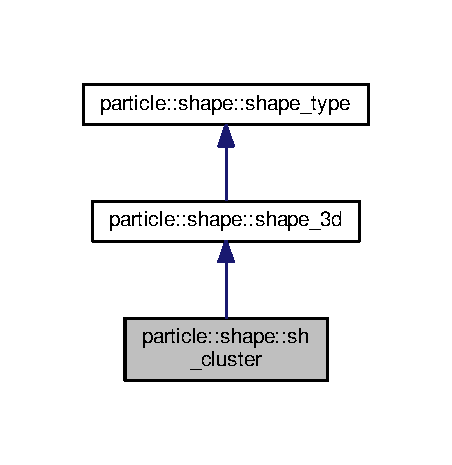
\includegraphics[width=217pt]{d8/d55/classparticle_1_1shape_1_1sh__cluster__inherit__graph}
\end{center}
\end{figure}


Collaboration diagram for particle\+:\+:shape\+:\+:sh\+\_\+cluster\+:\nopagebreak
\begin{figure}[H]
\begin{center}
\leavevmode
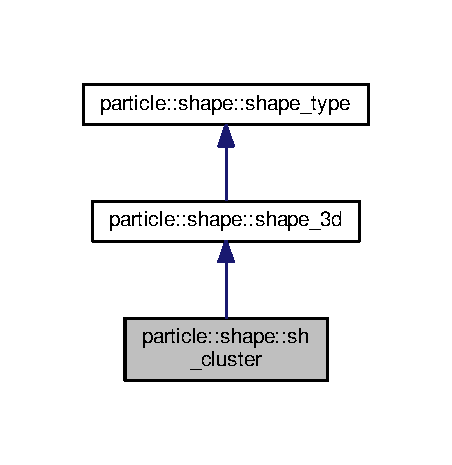
\includegraphics[width=217pt]{d6/d9e/classparticle_1_1shape_1_1sh__cluster__coll__graph}
\end{center}
\end{figure}
\subsection*{Public Member Functions}
\begin{DoxyCompactItemize}
\item 
\hyperlink{classparticle_1_1shape_1_1sh__cluster_a35768f3d2687ff2f178d465866fbb837}{sh\+\_\+cluster} ()
\begin{DoxyCompactList}\small\item\em Default constructor. \end{DoxyCompactList}\item 
\hyperlink{classparticle_1_1shape_1_1sh__cluster_acbb95a92e18fca21853a06c3c6d56524}{$\sim$sh\+\_\+cluster} ()
\begin{DoxyCompactList}\small\item\em Default destructor. \end{DoxyCompactList}\end{DoxyCompactItemize}


\subsection{Detailed Description}
Particle cluster (depreciated) 

\subsection{Constructor \& Destructor Documentation}
\index{particle\+::shape\+::sh\+\_\+cluster@{particle\+::shape\+::sh\+\_\+cluster}!sh\+\_\+cluster@{sh\+\_\+cluster}}
\index{sh\+\_\+cluster@{sh\+\_\+cluster}!particle\+::shape\+::sh\+\_\+cluster@{particle\+::shape\+::sh\+\_\+cluster}}
\subsubsection[{\texorpdfstring{sh\+\_\+cluster()}{sh_cluster()}}]{\setlength{\rightskip}{0pt plus 5cm}particle\+::shape\+::sh\+\_\+cluster\+::sh\+\_\+cluster (
\begin{DoxyParamCaption}
{}
\end{DoxyParamCaption}
)\hspace{0.3cm}{\ttfamily [inline]}}\hypertarget{classparticle_1_1shape_1_1sh__cluster_a35768f3d2687ff2f178d465866fbb837}{}\label{classparticle_1_1shape_1_1sh__cluster_a35768f3d2687ff2f178d465866fbb837}


Default constructor. 

\index{particle\+::shape\+::sh\+\_\+cluster@{particle\+::shape\+::sh\+\_\+cluster}!````~sh\+\_\+cluster@{$\sim$sh\+\_\+cluster}}
\index{````~sh\+\_\+cluster@{$\sim$sh\+\_\+cluster}!particle\+::shape\+::sh\+\_\+cluster@{particle\+::shape\+::sh\+\_\+cluster}}
\subsubsection[{\texorpdfstring{$\sim$sh\+\_\+cluster()}{~sh_cluster()}}]{\setlength{\rightskip}{0pt plus 5cm}particle\+::shape\+::sh\+\_\+cluster\+::$\sim$sh\+\_\+cluster (
\begin{DoxyParamCaption}
{}
\end{DoxyParamCaption}
)\hspace{0.3cm}{\ttfamily [inline]}}\hypertarget{classparticle_1_1shape_1_1sh__cluster_acbb95a92e18fca21853a06c3c6d56524}{}\label{classparticle_1_1shape_1_1sh__cluster_acbb95a92e18fca21853a06c3c6d56524}


Default destructor. 



The documentation for this class was generated from the following file\+:\begin{DoxyCompactItemize}
\item 
includes/\hyperlink{shape_8hpp}{shape.\+hpp}\end{DoxyCompactItemize}

\hypertarget{classparticle_1_1shape_1_1shape__2d}{}\section{particle\+:\+:shape\+:\+:shape\+\_\+2d Class Reference}
\label{classparticle_1_1shape_1_1shape__2d}\index{particle\+::shape\+::shape\+\_\+2d@{particle\+::shape\+::shape\+\_\+2d}}


2D particle shapes.  




{\ttfamily \#include $<$shape.\+hpp$>$}



Inheritance diagram for particle\+:\+:shape\+:\+:shape\+\_\+2d\+:\nopagebreak
\begin{figure}[H]
\begin{center}
\leavevmode
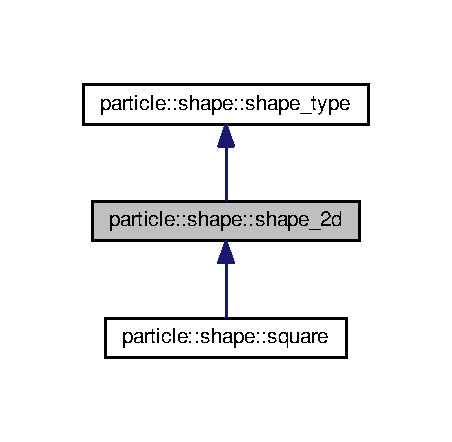
\includegraphics[width=217pt]{db/d00/classparticle_1_1shape_1_1shape__2d__inherit__graph}
\end{center}
\end{figure}


Collaboration diagram for particle\+:\+:shape\+:\+:shape\+\_\+2d\+:\nopagebreak
\begin{figure}[H]
\begin{center}
\leavevmode
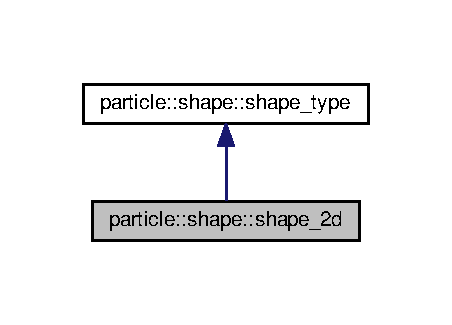
\includegraphics[width=217pt]{df/df8/classparticle_1_1shape_1_1shape__2d__coll__graph}
\end{center}
\end{figure}
\subsection*{Public Member Functions}
\begin{DoxyCompactItemize}
\item 
\hyperlink{classparticle_1_1shape_1_1shape__2d_a72d23ad24e5a3acc3948fbceb44591a4}{shape\+\_\+2d} ()
\begin{DoxyCompactList}\small\item\em Default constructor. \end{DoxyCompactList}\item 
\hyperlink{classparticle_1_1shape_1_1shape__2d_a6ea97cd4eedece84d77c9faa4fc960d2}{$\sim$shape\+\_\+2d} ()
\begin{DoxyCompactList}\small\item\em Default destructor. \end{DoxyCompactList}\item 
virtual bool \hyperlink{classparticle_1_1shape_1_1shape__2d_a756e06b46afd0e18d6a37a0a8f28551c}{check} (std\+::vector$<$ int $>$ Is, int l\+\_\+size)
\begin{DoxyCompactList}\small\item\em Check whether a certain position falls within the particle. \end{DoxyCompactList}\end{DoxyCompactItemize}


\subsection{Detailed Description}
2D particle shapes. 

\subsection{Constructor \& Destructor Documentation}
\index{particle\+::shape\+::shape\+\_\+2d@{particle\+::shape\+::shape\+\_\+2d}!shape\+\_\+2d@{shape\+\_\+2d}}
\index{shape\+\_\+2d@{shape\+\_\+2d}!particle\+::shape\+::shape\+\_\+2d@{particle\+::shape\+::shape\+\_\+2d}}
\subsubsection[{\texorpdfstring{shape\+\_\+2d()}{shape_2d()}}]{\setlength{\rightskip}{0pt plus 5cm}particle\+::shape\+::shape\+\_\+2d\+::shape\+\_\+2d (
\begin{DoxyParamCaption}
{}
\end{DoxyParamCaption}
)\hspace{0.3cm}{\ttfamily [inline]}}\hypertarget{classparticle_1_1shape_1_1shape__2d_a72d23ad24e5a3acc3948fbceb44591a4}{}\label{classparticle_1_1shape_1_1shape__2d_a72d23ad24e5a3acc3948fbceb44591a4}


Default constructor. 

\index{particle\+::shape\+::shape\+\_\+2d@{particle\+::shape\+::shape\+\_\+2d}!````~shape\+\_\+2d@{$\sim$shape\+\_\+2d}}
\index{````~shape\+\_\+2d@{$\sim$shape\+\_\+2d}!particle\+::shape\+::shape\+\_\+2d@{particle\+::shape\+::shape\+\_\+2d}}
\subsubsection[{\texorpdfstring{$\sim$shape\+\_\+2d()}{~shape_2d()}}]{\setlength{\rightskip}{0pt plus 5cm}particle\+::shape\+::shape\+\_\+2d\+::$\sim$shape\+\_\+2d (
\begin{DoxyParamCaption}
{}
\end{DoxyParamCaption}
)\hspace{0.3cm}{\ttfamily [inline]}}\hypertarget{classparticle_1_1shape_1_1shape__2d_a6ea97cd4eedece84d77c9faa4fc960d2}{}\label{classparticle_1_1shape_1_1shape__2d_a6ea97cd4eedece84d77c9faa4fc960d2}


Default destructor. 



\subsection{Member Function Documentation}
\index{particle\+::shape\+::shape\+\_\+2d@{particle\+::shape\+::shape\+\_\+2d}!check@{check}}
\index{check@{check}!particle\+::shape\+::shape\+\_\+2d@{particle\+::shape\+::shape\+\_\+2d}}
\subsubsection[{\texorpdfstring{check(std\+::vector$<$ int $>$ Is, int l\+\_\+size)}{check(std::vector< int > Is, int l_size)}}]{\setlength{\rightskip}{0pt plus 5cm}virtual bool particle\+::shape\+::shape\+\_\+2d\+::check (
\begin{DoxyParamCaption}
\item[{std\+::vector$<$ int $>$}]{Is, }
\item[{int}]{l\+\_\+size}
\end{DoxyParamCaption}
)\hspace{0.3cm}{\ttfamily [inline]}, {\ttfamily [virtual]}}\hypertarget{classparticle_1_1shape_1_1shape__2d_a756e06b46afd0e18d6a37a0a8f28551c}{}\label{classparticle_1_1shape_1_1shape__2d_a756e06b46afd0e18d6a37a0a8f28551c}


Check whether a certain position falls within the particle. 


\begin{DoxyParams}{Parameters}
{\em Is} & The coordinates of the lattice site. \\
\hline
{\em l\+\_\+size} & The total lattice size. \\
\hline
\end{DoxyParams}


Reimplemented from \hyperlink{classparticle_1_1shape_1_1shape__type_a64d04f49c8da656d8b8899c431c346fc}{particle\+::shape\+::shape\+\_\+type}.



The documentation for this class was generated from the following file\+:\begin{DoxyCompactItemize}
\item 
includes/\hyperlink{shape_8hpp}{shape.\+hpp}\end{DoxyCompactItemize}

\hypertarget{classparticle_1_1shape_1_1shape__3d}{}\section{particle\+:\+:shape\+:\+:shape\+\_\+3d Class Reference}
\label{classparticle_1_1shape_1_1shape__3d}\index{particle\+::shape\+::shape\+\_\+3d@{particle\+::shape\+::shape\+\_\+3d}}


3D particle shapes.  




{\ttfamily \#include $<$shape.\+hpp$>$}



Inheritance diagram for particle\+:\+:shape\+:\+:shape\+\_\+3d\+:\nopagebreak
\begin{figure}[H]
\begin{center}
\leavevmode
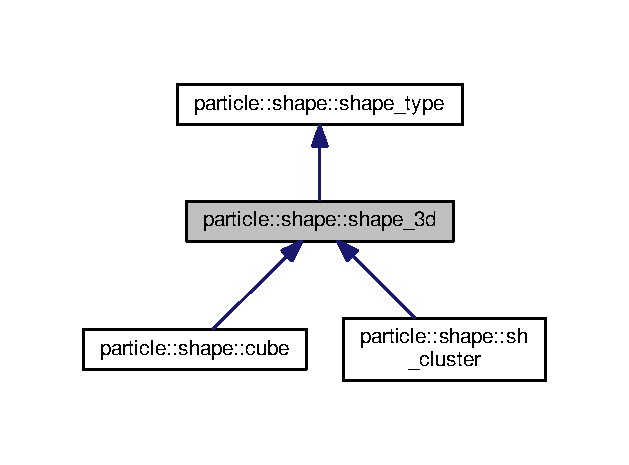
\includegraphics[width=302pt]{d4/dbf/classparticle_1_1shape_1_1shape__3d__inherit__graph}
\end{center}
\end{figure}


Collaboration diagram for particle\+:\+:shape\+:\+:shape\+\_\+3d\+:\nopagebreak
\begin{figure}[H]
\begin{center}
\leavevmode
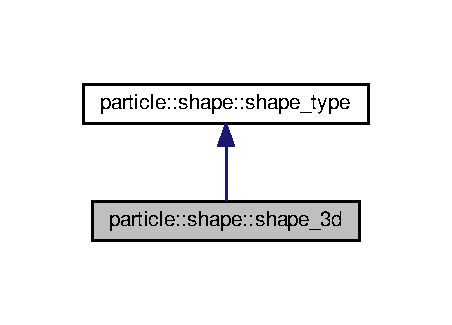
\includegraphics[width=217pt]{d1/d61/classparticle_1_1shape_1_1shape__3d__coll__graph}
\end{center}
\end{figure}
\subsection*{Public Member Functions}
\begin{DoxyCompactItemize}
\item 
\hyperlink{classparticle_1_1shape_1_1shape__3d_a5f7180f1f02937bf0b89e58229fb4848}{shape\+\_\+3d} ()
\begin{DoxyCompactList}\small\item\em Default constructor. \end{DoxyCompactList}\item 
\hyperlink{classparticle_1_1shape_1_1shape__3d_a9870c53de9607e6684f839f7b55058f9}{$\sim$shape\+\_\+3d} ()
\begin{DoxyCompactList}\small\item\em Default destructor. \end{DoxyCompactList}\item 
virtual bool \hyperlink{classparticle_1_1shape_1_1shape__3d_afa0d3025b8446a142b8979065eeb6379}{check} (std\+::vector$<$ int $>$ Is, int l\+\_\+size)
\begin{DoxyCompactList}\small\item\em Check whether a certain position falls within the particle. \end{DoxyCompactList}\end{DoxyCompactItemize}


\subsection{Detailed Description}
3D particle shapes. 

\subsection{Constructor \& Destructor Documentation}
\index{particle\+::shape\+::shape\+\_\+3d@{particle\+::shape\+::shape\+\_\+3d}!shape\+\_\+3d@{shape\+\_\+3d}}
\index{shape\+\_\+3d@{shape\+\_\+3d}!particle\+::shape\+::shape\+\_\+3d@{particle\+::shape\+::shape\+\_\+3d}}
\subsubsection[{\texorpdfstring{shape\+\_\+3d()}{shape_3d()}}]{\setlength{\rightskip}{0pt plus 5cm}particle\+::shape\+::shape\+\_\+3d\+::shape\+\_\+3d (
\begin{DoxyParamCaption}
{}
\end{DoxyParamCaption}
)\hspace{0.3cm}{\ttfamily [inline]}}\hypertarget{classparticle_1_1shape_1_1shape__3d_a5f7180f1f02937bf0b89e58229fb4848}{}\label{classparticle_1_1shape_1_1shape__3d_a5f7180f1f02937bf0b89e58229fb4848}


Default constructor. 

\index{particle\+::shape\+::shape\+\_\+3d@{particle\+::shape\+::shape\+\_\+3d}!````~shape\+\_\+3d@{$\sim$shape\+\_\+3d}}
\index{````~shape\+\_\+3d@{$\sim$shape\+\_\+3d}!particle\+::shape\+::shape\+\_\+3d@{particle\+::shape\+::shape\+\_\+3d}}
\subsubsection[{\texorpdfstring{$\sim$shape\+\_\+3d()}{~shape_3d()}}]{\setlength{\rightskip}{0pt plus 5cm}particle\+::shape\+::shape\+\_\+3d\+::$\sim$shape\+\_\+3d (
\begin{DoxyParamCaption}
{}
\end{DoxyParamCaption}
)\hspace{0.3cm}{\ttfamily [inline]}}\hypertarget{classparticle_1_1shape_1_1shape__3d_a9870c53de9607e6684f839f7b55058f9}{}\label{classparticle_1_1shape_1_1shape__3d_a9870c53de9607e6684f839f7b55058f9}


Default destructor. 



\subsection{Member Function Documentation}
\index{particle\+::shape\+::shape\+\_\+3d@{particle\+::shape\+::shape\+\_\+3d}!check@{check}}
\index{check@{check}!particle\+::shape\+::shape\+\_\+3d@{particle\+::shape\+::shape\+\_\+3d}}
\subsubsection[{\texorpdfstring{check(std\+::vector$<$ int $>$ Is, int l\+\_\+size)}{check(std::vector< int > Is, int l_size)}}]{\setlength{\rightskip}{0pt plus 5cm}virtual bool particle\+::shape\+::shape\+\_\+3d\+::check (
\begin{DoxyParamCaption}
\item[{std\+::vector$<$ int $>$}]{Is, }
\item[{int}]{l\+\_\+size}
\end{DoxyParamCaption}
)\hspace{0.3cm}{\ttfamily [inline]}, {\ttfamily [virtual]}}\hypertarget{classparticle_1_1shape_1_1shape__3d_afa0d3025b8446a142b8979065eeb6379}{}\label{classparticle_1_1shape_1_1shape__3d_afa0d3025b8446a142b8979065eeb6379}


Check whether a certain position falls within the particle. 


\begin{DoxyParams}{Parameters}
{\em Is} & The coordinates of the lattice site. \\
\hline
{\em l\+\_\+size} & The total lattice size. \\
\hline
\end{DoxyParams}


Reimplemented from \hyperlink{classparticle_1_1shape_1_1shape__type_a64d04f49c8da656d8b8899c431c346fc}{particle\+::shape\+::shape\+\_\+type}.



The documentation for this class was generated from the following file\+:\begin{DoxyCompactItemize}
\item 
includes/\hyperlink{shape_8hpp}{shape.\+hpp}\end{DoxyCompactItemize}

\hypertarget{classparticle_1_1shape_1_1shape__type}{}\section{particle\+:\+:shape\+:\+:shape\+\_\+type Class Reference}
\label{classparticle_1_1shape_1_1shape__type}\index{particle\+::shape\+::shape\+\_\+type@{particle\+::shape\+::shape\+\_\+type}}


Base class for particle shapes.  




{\ttfamily \#include $<$shape.\+hpp$>$}



Inheritance diagram for particle\+:\+:shape\+:\+:shape\+\_\+type\+:\nopagebreak
\begin{figure}[H]
\begin{center}
\leavevmode
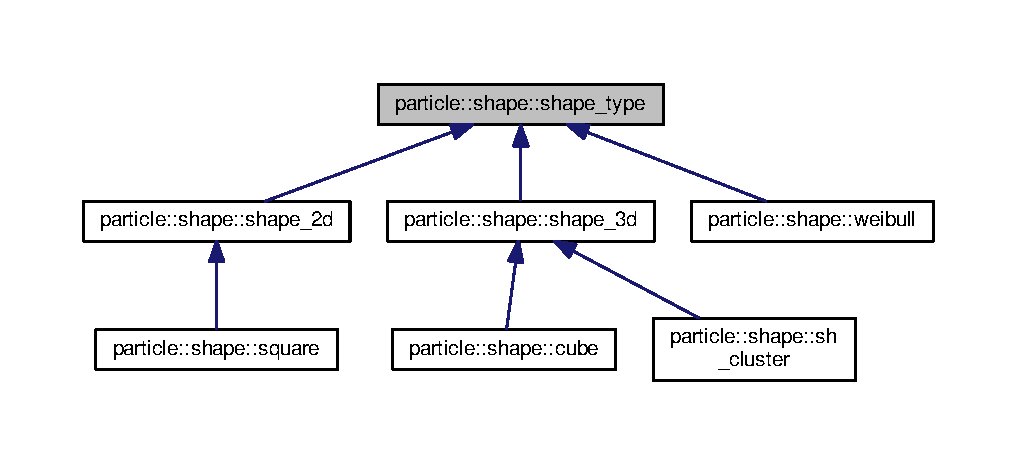
\includegraphics[width=350pt]{d6/d08/classparticle_1_1shape_1_1shape__type__inherit__graph}
\end{center}
\end{figure}
\subsection*{Public Member Functions}
\begin{DoxyCompactItemize}
\item 
\hyperlink{classparticle_1_1shape_1_1shape__type_ab187327a7f6a06f60f4714395f3eca88}{shape\+\_\+type} ()
\begin{DoxyCompactList}\small\item\em Default constructor. \end{DoxyCompactList}\item 
\hyperlink{classparticle_1_1shape_1_1shape__type_a86b549bc6531e04873ca057172ec3f0f}{$\sim$shape\+\_\+type} ()
\begin{DoxyCompactList}\small\item\em Default destructor. \end{DoxyCompactList}\item 
virtual bool \hyperlink{classparticle_1_1shape_1_1shape__type_a64d04f49c8da656d8b8899c431c346fc}{check} (std\+::vector$<$ int $>$ Is, int l\+\_\+size)
\begin{DoxyCompactList}\small\item\em Check whether a certain position falls within the particle. \end{DoxyCompactList}\item 
virtual double \hyperlink{classparticle_1_1shape_1_1shape__type_a062dfaf9cbfe98cdcdc55c34a0463313}{get\+\_\+r0} ()
\begin{DoxyCompactList}\small\item\em Returns the characteristic size of a weibull particle. \end{DoxyCompactList}\item 
virtual double \hyperlink{classparticle_1_1shape_1_1shape__type_a041dd08774f26ffeeb051e1442cb612c}{get\+\_\+beta} ()
\begin{DoxyCompactList}\small\item\em Returns the disorder parameter of a weibull particle. \end{DoxyCompactList}\item 
virtual double \hyperlink{classparticle_1_1shape_1_1shape__type_a7b938aa8c2dada71e8d0b11c6a676449}{get\+\_\+a} ()
\begin{DoxyCompactList}\small\item\em Returns the x-\/axis radius of a weibull particle. \end{DoxyCompactList}\item 
virtual double \hyperlink{classparticle_1_1shape_1_1shape__type_a0a9f0a397edbc66120114c89a185c127}{get\+\_\+b} ()
\begin{DoxyCompactList}\small\item\em Returns the y-\/axis radius of a weibull particle. \end{DoxyCompactList}\item 
virtual double \hyperlink{classparticle_1_1shape_1_1shape__type_a4f37d43b6e014a429e45480cea48f63d}{get\+\_\+c} ()
\begin{DoxyCompactList}\small\item\em Returns the z-\/axis radius of a weibull particle. \end{DoxyCompactList}\end{DoxyCompactItemize}


\subsection{Detailed Description}
Base class for particle shapes. 

\subsection{Constructor \& Destructor Documentation}
\index{particle\+::shape\+::shape\+\_\+type@{particle\+::shape\+::shape\+\_\+type}!shape\+\_\+type@{shape\+\_\+type}}
\index{shape\+\_\+type@{shape\+\_\+type}!particle\+::shape\+::shape\+\_\+type@{particle\+::shape\+::shape\+\_\+type}}
\subsubsection[{\texorpdfstring{shape\+\_\+type()}{shape_type()}}]{\setlength{\rightskip}{0pt plus 5cm}particle\+::shape\+::shape\+\_\+type\+::shape\+\_\+type (
\begin{DoxyParamCaption}
{}
\end{DoxyParamCaption}
)\hspace{0.3cm}{\ttfamily [inline]}}\hypertarget{classparticle_1_1shape_1_1shape__type_ab187327a7f6a06f60f4714395f3eca88}{}\label{classparticle_1_1shape_1_1shape__type_ab187327a7f6a06f60f4714395f3eca88}


Default constructor. 

\index{particle\+::shape\+::shape\+\_\+type@{particle\+::shape\+::shape\+\_\+type}!````~shape\+\_\+type@{$\sim$shape\+\_\+type}}
\index{````~shape\+\_\+type@{$\sim$shape\+\_\+type}!particle\+::shape\+::shape\+\_\+type@{particle\+::shape\+::shape\+\_\+type}}
\subsubsection[{\texorpdfstring{$\sim$shape\+\_\+type()}{~shape_type()}}]{\setlength{\rightskip}{0pt plus 5cm}particle\+::shape\+::shape\+\_\+type\+::$\sim$shape\+\_\+type (
\begin{DoxyParamCaption}
{}
\end{DoxyParamCaption}
)\hspace{0.3cm}{\ttfamily [inline]}}\hypertarget{classparticle_1_1shape_1_1shape__type_a86b549bc6531e04873ca057172ec3f0f}{}\label{classparticle_1_1shape_1_1shape__type_a86b549bc6531e04873ca057172ec3f0f}


Default destructor. 



\subsection{Member Function Documentation}
\index{particle\+::shape\+::shape\+\_\+type@{particle\+::shape\+::shape\+\_\+type}!check@{check}}
\index{check@{check}!particle\+::shape\+::shape\+\_\+type@{particle\+::shape\+::shape\+\_\+type}}
\subsubsection[{\texorpdfstring{check(std\+::vector$<$ int $>$ Is, int l\+\_\+size)}{check(std::vector< int > Is, int l_size)}}]{\setlength{\rightskip}{0pt plus 5cm}virtual bool particle\+::shape\+::shape\+\_\+type\+::check (
\begin{DoxyParamCaption}
\item[{std\+::vector$<$ int $>$}]{Is, }
\item[{int}]{l\+\_\+size}
\end{DoxyParamCaption}
)\hspace{0.3cm}{\ttfamily [inline]}, {\ttfamily [virtual]}}\hypertarget{classparticle_1_1shape_1_1shape__type_a64d04f49c8da656d8b8899c431c346fc}{}\label{classparticle_1_1shape_1_1shape__type_a64d04f49c8da656d8b8899c431c346fc}


Check whether a certain position falls within the particle. 


\begin{DoxyParams}{Parameters}
{\em Is} & The coordinates of the lattice site. \\
\hline
{\em l\+\_\+size} & The total lattice size. \\
\hline
\end{DoxyParams}


Reimplemented in \hyperlink{classparticle_1_1shape_1_1weibull_a22612311ce2f3ca4317f8263e52de425}{particle\+::shape\+::weibull}, \hyperlink{classparticle_1_1shape_1_1shape__3d_afa0d3025b8446a142b8979065eeb6379}{particle\+::shape\+::shape\+\_\+3d}, and \hyperlink{classparticle_1_1shape_1_1shape__2d_a756e06b46afd0e18d6a37a0a8f28551c}{particle\+::shape\+::shape\+\_\+2d}.

\index{particle\+::shape\+::shape\+\_\+type@{particle\+::shape\+::shape\+\_\+type}!get\+\_\+a@{get\+\_\+a}}
\index{get\+\_\+a@{get\+\_\+a}!particle\+::shape\+::shape\+\_\+type@{particle\+::shape\+::shape\+\_\+type}}
\subsubsection[{\texorpdfstring{get\+\_\+a()}{get_a()}}]{\setlength{\rightskip}{0pt plus 5cm}virtual double particle\+::shape\+::shape\+\_\+type\+::get\+\_\+a (
\begin{DoxyParamCaption}
{}
\end{DoxyParamCaption}
)\hspace{0.3cm}{\ttfamily [inline]}, {\ttfamily [virtual]}}\hypertarget{classparticle_1_1shape_1_1shape__type_a7b938aa8c2dada71e8d0b11c6a676449}{}\label{classparticle_1_1shape_1_1shape__type_a7b938aa8c2dada71e8d0b11c6a676449}


Returns the x-\/axis radius of a weibull particle. 



Reimplemented in \hyperlink{classparticle_1_1shape_1_1weibull_a0234fa42b67465c7191248f524f27a0e}{particle\+::shape\+::weibull}.

\index{particle\+::shape\+::shape\+\_\+type@{particle\+::shape\+::shape\+\_\+type}!get\+\_\+b@{get\+\_\+b}}
\index{get\+\_\+b@{get\+\_\+b}!particle\+::shape\+::shape\+\_\+type@{particle\+::shape\+::shape\+\_\+type}}
\subsubsection[{\texorpdfstring{get\+\_\+b()}{get_b()}}]{\setlength{\rightskip}{0pt plus 5cm}virtual double particle\+::shape\+::shape\+\_\+type\+::get\+\_\+b (
\begin{DoxyParamCaption}
{}
\end{DoxyParamCaption}
)\hspace{0.3cm}{\ttfamily [inline]}, {\ttfamily [virtual]}}\hypertarget{classparticle_1_1shape_1_1shape__type_a0a9f0a397edbc66120114c89a185c127}{}\label{classparticle_1_1shape_1_1shape__type_a0a9f0a397edbc66120114c89a185c127}


Returns the y-\/axis radius of a weibull particle. 



Reimplemented in \hyperlink{classparticle_1_1shape_1_1weibull_a1066adcab828f8636475128ff51c56f0}{particle\+::shape\+::weibull}.

\index{particle\+::shape\+::shape\+\_\+type@{particle\+::shape\+::shape\+\_\+type}!get\+\_\+beta@{get\+\_\+beta}}
\index{get\+\_\+beta@{get\+\_\+beta}!particle\+::shape\+::shape\+\_\+type@{particle\+::shape\+::shape\+\_\+type}}
\subsubsection[{\texorpdfstring{get\+\_\+beta()}{get_beta()}}]{\setlength{\rightskip}{0pt plus 5cm}virtual double particle\+::shape\+::shape\+\_\+type\+::get\+\_\+beta (
\begin{DoxyParamCaption}
{}
\end{DoxyParamCaption}
)\hspace{0.3cm}{\ttfamily [inline]}, {\ttfamily [virtual]}}\hypertarget{classparticle_1_1shape_1_1shape__type_a041dd08774f26ffeeb051e1442cb612c}{}\label{classparticle_1_1shape_1_1shape__type_a041dd08774f26ffeeb051e1442cb612c}


Returns the disorder parameter of a weibull particle. 



Reimplemented in \hyperlink{classparticle_1_1shape_1_1weibull_a640180ce2bd6ce7f68c10d4791bce49c}{particle\+::shape\+::weibull}.

\index{particle\+::shape\+::shape\+\_\+type@{particle\+::shape\+::shape\+\_\+type}!get\+\_\+c@{get\+\_\+c}}
\index{get\+\_\+c@{get\+\_\+c}!particle\+::shape\+::shape\+\_\+type@{particle\+::shape\+::shape\+\_\+type}}
\subsubsection[{\texorpdfstring{get\+\_\+c()}{get_c()}}]{\setlength{\rightskip}{0pt plus 5cm}virtual double particle\+::shape\+::shape\+\_\+type\+::get\+\_\+c (
\begin{DoxyParamCaption}
{}
\end{DoxyParamCaption}
)\hspace{0.3cm}{\ttfamily [inline]}, {\ttfamily [virtual]}}\hypertarget{classparticle_1_1shape_1_1shape__type_a4f37d43b6e014a429e45480cea48f63d}{}\label{classparticle_1_1shape_1_1shape__type_a4f37d43b6e014a429e45480cea48f63d}


Returns the z-\/axis radius of a weibull particle. 



Reimplemented in \hyperlink{classparticle_1_1shape_1_1weibull_a0b8c38944e502df7bce4e8f99d149237}{particle\+::shape\+::weibull}.

\index{particle\+::shape\+::shape\+\_\+type@{particle\+::shape\+::shape\+\_\+type}!get\+\_\+r0@{get\+\_\+r0}}
\index{get\+\_\+r0@{get\+\_\+r0}!particle\+::shape\+::shape\+\_\+type@{particle\+::shape\+::shape\+\_\+type}}
\subsubsection[{\texorpdfstring{get\+\_\+r0()}{get_r0()}}]{\setlength{\rightskip}{0pt plus 5cm}virtual double particle\+::shape\+::shape\+\_\+type\+::get\+\_\+r0 (
\begin{DoxyParamCaption}
{}
\end{DoxyParamCaption}
)\hspace{0.3cm}{\ttfamily [inline]}, {\ttfamily [virtual]}}\hypertarget{classparticle_1_1shape_1_1shape__type_a062dfaf9cbfe98cdcdc55c34a0463313}{}\label{classparticle_1_1shape_1_1shape__type_a062dfaf9cbfe98cdcdc55c34a0463313}


Returns the characteristic size of a weibull particle. 



Reimplemented in \hyperlink{classparticle_1_1shape_1_1weibull_a85ab45f804ae9aa3fb712c435125ff70}{particle\+::shape\+::weibull}.



The documentation for this class was generated from the following file\+:\begin{DoxyCompactItemize}
\item 
includes/\hyperlink{shape_8hpp}{shape.\+hpp}\end{DoxyCompactItemize}

\hypertarget{structsimOptions}{}\section{sim\+Options Struct Reference}
\label{structsimOptions}\index{sim\+Options@{sim\+Options}}


{\ttfamily \#include $<$param\+\_\+read.\+hpp$>$}

\subsection*{Public Attributes}
\begin{DoxyCompactItemize}
\item 
std\+::string \hyperlink{structsimOptions_a42a20f246c7029967d29a15e4d5aac16}{temp\+File}
\item 
std\+::string \hyperlink{structsimOptions_afb799330b8e40d76661b590ce0e792e6}{field\+File}
\item 
std\+::string \hyperlink{structsimOptions_ad95991f4f13947624c4e44ea12845c18}{out\+File}
\item 
int \hyperlink{structsimOptions_a5890487eea2252d4d84f67615269128f}{Samp\+\_\+steps}
\item 
int \hyperlink{structsimOptions_a94b0e70bb9de2b53a815b67879929b65}{N\+\_\+samp}
\item 
int \hyperlink{structsimOptions_a68e2dc1a21bc70873cdd518cf90b01f0}{Eq\+\_\+steps}
\item 
int \hyperlink{structsimOptions_a22e632d6787e16c4a95781ea672184ba}{N\+\_\+latts}
\item 
int \hyperlink{structsimOptions_a0b1b41d907adf31c75d5b9e9a413931d}{protocol}
\item 
bool \hyperlink{structsimOptions_ac515e118d7c1c579e0cf9e789c1c6926}{distrib}
\item 
double \hyperlink{structsimOptions_a8af2a6dac9cbe680605b83147dca9b96}{amean}
\item 
double \hyperlink{structsimOptions_a97b27544bdce1f29971f1501a15a3fe5}{asd}
\item 
double \hyperlink{structsimOptions_a4f77eb0b474df8666c76e29c322d4276}{lmean}
\item 
double \hyperlink{structsimOptions_aa167da0ff74e6ba414e67213f67abd2f}{lsd}
\end{DoxyCompactItemize}


\subsection{Member Data Documentation}
\index{sim\+Options@{sim\+Options}!amean@{amean}}
\index{amean@{amean}!sim\+Options@{sim\+Options}}
\subsubsection[{\texorpdfstring{amean}{amean}}]{\setlength{\rightskip}{0pt plus 5cm}double sim\+Options\+::amean}\hypertarget{structsimOptions_a8af2a6dac9cbe680605b83147dca9b96}{}\label{structsimOptions_a8af2a6dac9cbe680605b83147dca9b96}
\index{sim\+Options@{sim\+Options}!asd@{asd}}
\index{asd@{asd}!sim\+Options@{sim\+Options}}
\subsubsection[{\texorpdfstring{asd}{asd}}]{\setlength{\rightskip}{0pt plus 5cm}double sim\+Options\+::asd}\hypertarget{structsimOptions_a97b27544bdce1f29971f1501a15a3fe5}{}\label{structsimOptions_a97b27544bdce1f29971f1501a15a3fe5}
\index{sim\+Options@{sim\+Options}!distrib@{distrib}}
\index{distrib@{distrib}!sim\+Options@{sim\+Options}}
\subsubsection[{\texorpdfstring{distrib}{distrib}}]{\setlength{\rightskip}{0pt plus 5cm}bool sim\+Options\+::distrib}\hypertarget{structsimOptions_ac515e118d7c1c579e0cf9e789c1c6926}{}\label{structsimOptions_ac515e118d7c1c579e0cf9e789c1c6926}
\index{sim\+Options@{sim\+Options}!Eq\+\_\+steps@{Eq\+\_\+steps}}
\index{Eq\+\_\+steps@{Eq\+\_\+steps}!sim\+Options@{sim\+Options}}
\subsubsection[{\texorpdfstring{Eq\+\_\+steps}{Eq_steps}}]{\setlength{\rightskip}{0pt plus 5cm}int sim\+Options\+::\+Eq\+\_\+steps}\hypertarget{structsimOptions_a68e2dc1a21bc70873cdd518cf90b01f0}{}\label{structsimOptions_a68e2dc1a21bc70873cdd518cf90b01f0}
\index{sim\+Options@{sim\+Options}!field\+File@{field\+File}}
\index{field\+File@{field\+File}!sim\+Options@{sim\+Options}}
\subsubsection[{\texorpdfstring{field\+File}{fieldFile}}]{\setlength{\rightskip}{0pt plus 5cm}std\+::string sim\+Options\+::field\+File}\hypertarget{structsimOptions_afb799330b8e40d76661b590ce0e792e6}{}\label{structsimOptions_afb799330b8e40d76661b590ce0e792e6}
\index{sim\+Options@{sim\+Options}!lmean@{lmean}}
\index{lmean@{lmean}!sim\+Options@{sim\+Options}}
\subsubsection[{\texorpdfstring{lmean}{lmean}}]{\setlength{\rightskip}{0pt plus 5cm}double sim\+Options\+::lmean}\hypertarget{structsimOptions_a4f77eb0b474df8666c76e29c322d4276}{}\label{structsimOptions_a4f77eb0b474df8666c76e29c322d4276}
\index{sim\+Options@{sim\+Options}!lsd@{lsd}}
\index{lsd@{lsd}!sim\+Options@{sim\+Options}}
\subsubsection[{\texorpdfstring{lsd}{lsd}}]{\setlength{\rightskip}{0pt plus 5cm}double sim\+Options\+::lsd}\hypertarget{structsimOptions_aa167da0ff74e6ba414e67213f67abd2f}{}\label{structsimOptions_aa167da0ff74e6ba414e67213f67abd2f}
\index{sim\+Options@{sim\+Options}!N\+\_\+latts@{N\+\_\+latts}}
\index{N\+\_\+latts@{N\+\_\+latts}!sim\+Options@{sim\+Options}}
\subsubsection[{\texorpdfstring{N\+\_\+latts}{N_latts}}]{\setlength{\rightskip}{0pt plus 5cm}int sim\+Options\+::\+N\+\_\+latts}\hypertarget{structsimOptions_a22e632d6787e16c4a95781ea672184ba}{}\label{structsimOptions_a22e632d6787e16c4a95781ea672184ba}
\index{sim\+Options@{sim\+Options}!N\+\_\+samp@{N\+\_\+samp}}
\index{N\+\_\+samp@{N\+\_\+samp}!sim\+Options@{sim\+Options}}
\subsubsection[{\texorpdfstring{N\+\_\+samp}{N_samp}}]{\setlength{\rightskip}{0pt plus 5cm}int sim\+Options\+::\+N\+\_\+samp}\hypertarget{structsimOptions_a94b0e70bb9de2b53a815b67879929b65}{}\label{structsimOptions_a94b0e70bb9de2b53a815b67879929b65}
\index{sim\+Options@{sim\+Options}!out\+File@{out\+File}}
\index{out\+File@{out\+File}!sim\+Options@{sim\+Options}}
\subsubsection[{\texorpdfstring{out\+File}{outFile}}]{\setlength{\rightskip}{0pt plus 5cm}std\+::string sim\+Options\+::out\+File}\hypertarget{structsimOptions_ad95991f4f13947624c4e44ea12845c18}{}\label{structsimOptions_ad95991f4f13947624c4e44ea12845c18}
\index{sim\+Options@{sim\+Options}!protocol@{protocol}}
\index{protocol@{protocol}!sim\+Options@{sim\+Options}}
\subsubsection[{\texorpdfstring{protocol}{protocol}}]{\setlength{\rightskip}{0pt plus 5cm}int sim\+Options\+::protocol}\hypertarget{structsimOptions_a0b1b41d907adf31c75d5b9e9a413931d}{}\label{structsimOptions_a0b1b41d907adf31c75d5b9e9a413931d}
\index{sim\+Options@{sim\+Options}!Samp\+\_\+steps@{Samp\+\_\+steps}}
\index{Samp\+\_\+steps@{Samp\+\_\+steps}!sim\+Options@{sim\+Options}}
\subsubsection[{\texorpdfstring{Samp\+\_\+steps}{Samp_steps}}]{\setlength{\rightskip}{0pt plus 5cm}int sim\+Options\+::\+Samp\+\_\+steps}\hypertarget{structsimOptions_a5890487eea2252d4d84f67615269128f}{}\label{structsimOptions_a5890487eea2252d4d84f67615269128f}
\index{sim\+Options@{sim\+Options}!temp\+File@{temp\+File}}
\index{temp\+File@{temp\+File}!sim\+Options@{sim\+Options}}
\subsubsection[{\texorpdfstring{temp\+File}{tempFile}}]{\setlength{\rightskip}{0pt plus 5cm}std\+::string sim\+Options\+::temp\+File}\hypertarget{structsimOptions_a42a20f246c7029967d29a15e4d5aac16}{}\label{structsimOptions_a42a20f246c7029967d29a15e4d5aac16}


The documentation for this struct was generated from the following file\+:\begin{DoxyCompactItemize}
\item 
includes/\hyperlink{param__read_8hpp}{param\+\_\+read.\+hpp}\end{DoxyCompactItemize}

\hypertarget{classparticle_1_1shape_1_1square}{}\section{particle\+:\+:shape\+:\+:square Class Reference}
\label{classparticle_1_1shape_1_1square}\index{particle\+::shape\+::square@{particle\+::shape\+::square}}


Square particle.  




{\ttfamily \#include $<$shape.\+hpp$>$}



Inheritance diagram for particle\+:\+:shape\+:\+:square\+:\nopagebreak
\begin{figure}[H]
\begin{center}
\leavevmode
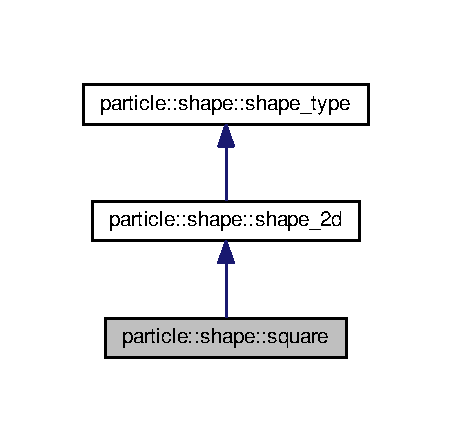
\includegraphics[width=217pt]{dd/d48/classparticle_1_1shape_1_1square__inherit__graph}
\end{center}
\end{figure}


Collaboration diagram for particle\+:\+:shape\+:\+:square\+:\nopagebreak
\begin{figure}[H]
\begin{center}
\leavevmode
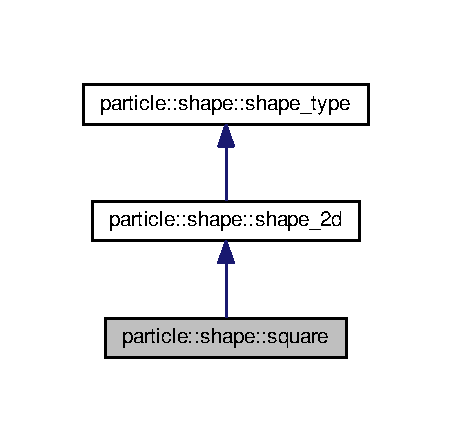
\includegraphics[width=217pt]{dd/d79/classparticle_1_1shape_1_1square__coll__graph}
\end{center}
\end{figure}
\subsection*{Public Member Functions}
\begin{DoxyCompactItemize}
\item 
\hyperlink{classparticle_1_1shape_1_1square_ad20d36cae1a25b17f151e194cca2933a}{square} ()
\begin{DoxyCompactList}\small\item\em Default constructor. \end{DoxyCompactList}\item 
\hyperlink{classparticle_1_1shape_1_1square_a2c16c3c04400bc8db355ea4d0ed2d2ec}{$\sim$square} ()
\begin{DoxyCompactList}\small\item\em Default destructor. \end{DoxyCompactList}\end{DoxyCompactItemize}


\subsection{Detailed Description}
Square particle. 

\subsection{Constructor \& Destructor Documentation}
\index{particle\+::shape\+::square@{particle\+::shape\+::square}!square@{square}}
\index{square@{square}!particle\+::shape\+::square@{particle\+::shape\+::square}}
\subsubsection[{\texorpdfstring{square()}{square()}}]{\setlength{\rightskip}{0pt plus 5cm}particle\+::shape\+::square\+::square (
\begin{DoxyParamCaption}
{}
\end{DoxyParamCaption}
)\hspace{0.3cm}{\ttfamily [inline]}}\hypertarget{classparticle_1_1shape_1_1square_ad20d36cae1a25b17f151e194cca2933a}{}\label{classparticle_1_1shape_1_1square_ad20d36cae1a25b17f151e194cca2933a}


Default constructor. 

\index{particle\+::shape\+::square@{particle\+::shape\+::square}!````~square@{$\sim$square}}
\index{````~square@{$\sim$square}!particle\+::shape\+::square@{particle\+::shape\+::square}}
\subsubsection[{\texorpdfstring{$\sim$square()}{~square()}}]{\setlength{\rightskip}{0pt plus 5cm}particle\+::shape\+::square\+::$\sim$square (
\begin{DoxyParamCaption}
{}
\end{DoxyParamCaption}
)\hspace{0.3cm}{\ttfamily [inline]}}\hypertarget{classparticle_1_1shape_1_1square_a2c16c3c04400bc8db355ea4d0ed2d2ec}{}\label{classparticle_1_1shape_1_1square_a2c16c3c04400bc8db355ea4d0ed2d2ec}


Default destructor. 



The documentation for this class was generated from the following file\+:\begin{DoxyCompactItemize}
\item 
includes/\hyperlink{shape_8hpp}{shape.\+hpp}\end{DoxyCompactItemize}

\hypertarget{classstate}{}\section{state Class Reference}
\label{classstate}\index{state@{state}}


{\ttfamily \#include $<$state.\+hpp$>$}

\subsection*{Public Member Functions}
\begin{DoxyCompactItemize}
\item 
\hyperlink{classstate_aee920d9f534640451f22b3525f9cb9de}{state} ()
\item 
\hyperlink{classstate_aa3dee783102d59b3c07617558c25afaf}{state} (\hyperlink{structstateOptions}{state\+Options} opt)
\item 
\hyperlink{classstate_a285d976cdbd4a9de9ec8d1d887991ecc}{state} (const \hyperlink{classstate}{state} \&other)
\item 
\hyperlink{classstate_a60216b51b01ca0ebe9786ec2da66568f}{$\sim$state} ()
\item 
\hyperlink{classparticle_1_1field_1_1field__type}{particle\+::field\+::field\+\_\+type} \hyperlink{classstate_a0a6f3f9510acca9b766cc4b4f17671c0}{get\+\_\+field} ()
\item 
void \hyperlink{classstate_a0d0ea6448509ececead44d83b4decd1c}{copy\+\_\+points} (const \hyperlink{classstate}{state} \&other)
\item 
void \hyperlink{classstate_aac3b2330539154d3784730e4c8a61123}{init\+\_\+points} (\hyperlink{structstateOptions}{state\+Options} opt)
\item 
void \hyperlink{classstate_af70b6f999313cc427a526388058cb45c}{equil} (int iter)
\item 
std\+::vector$<$ double $>$ \hyperlink{classstate_a5d5980e59b16063808f09eac46d14292}{magnetisation} ()
\item 
std\+::vector$<$ double $>$ \hyperlink{classstate_aff62d62706dc27dde2c3638769c0a00a}{submag} (int subnumber)
\item 
double \hyperlink{classstate_a6209503f752e5089e0301f103fdf1d1e}{energy} ()
\item 
std\+::vector$<$ double $>$ \hyperlink{classstate_aba4b4f47fc3b9cba97b5f63518214f30}{tcharge} ()
\item 
int \hyperlink{classstate_ad9182b875a7a3fb5981c811f7f062040}{num\+\_\+spins} ()
\item 
int \hyperlink{classstate_acf2ec1dfdb1068a279de590375cbcb96}{get\+\_\+size} ()
\item 
int \hyperlink{classstate_a8351befda232e04536d6a3e738754282}{sub\+\_\+num} (int subnumber)
\item 
void \hyperlink{classstate_acfeea4e197f5ce0160c6c664740ba6ff}{init\+\_\+lattice} ()
\item 
void \hyperlink{classstate_aca18a3757a2e6bd79cda366e4e31bb99}{change\+\_\+temp} (double T)
\item 
void \hyperlink{classstate_a3f54c8647fddb251db2ba11420f4e75f}{change\+\_\+field} (double Hin)
\item 
\hyperlink{classstate}{state} \& \hyperlink{classstate_a8f382a578a92617e7294cbbd80fba3c6}{operator=} (const \hyperlink{classstate}{state} \&other)
\item 
void \hyperlink{classstate_afa18f63b166492174bf88cd52c1cb748}{print\+\_\+latt} ()
\item 
void \hyperlink{classstate_af478dc8ce44c65cc535530738693eff5}{ptf} (std\+::string fname, std\+::string arrname)
\item 
void \hyperlink{classstate_a2d9073df186ccbf4159022d1c8c3b061}{add\+\_\+to\+\_\+av} (\hyperlink{classparticle_1_1field_1_1field__type}{particle\+::field\+::field\+\_\+type} \&other\+\_\+field)
\item 
void \hyperlink{classstate_a74588f49ec2b0868442d78ed9dcf1224}{change\+\_\+v1} (int protocol, double v1)
\item 
void \hyperlink{classstate_a9ffa7fbd21b542e66a9275f63b80ed0a}{change\+\_\+v2} (int protocol, double v2)
\item 
void \hyperlink{classstate_a6e35e024e6139032a54099bfe84a6fa4}{send\+\_\+latt\+\_\+data} (int dest\+\_\+rank)
\item 
void \hyperlink{classstate_a5ce0ea314795d1cc37849604f202fb98}{recv\+\_\+latt\+\_\+data} (int src\+\_\+rank)
\end{DoxyCompactItemize}


\subsection{Constructor \& Destructor Documentation}
\index{state@{state}!state@{state}}
\index{state@{state}!state@{state}}
\subsubsection[{\texorpdfstring{state()}{state()}}]{\setlength{\rightskip}{0pt plus 5cm}state\+::state (
\begin{DoxyParamCaption}
{}
\end{DoxyParamCaption}
)\hspace{0.3cm}{\ttfamily [inline]}}\hypertarget{classstate_aee920d9f534640451f22b3525f9cb9de}{}\label{classstate_aee920d9f534640451f22b3525f9cb9de}
\index{state@{state}!state@{state}}
\index{state@{state}!state@{state}}
\subsubsection[{\texorpdfstring{state(state\+Options opt)}{state(stateOptions opt)}}]{\setlength{\rightskip}{0pt plus 5cm}state\+::state (
\begin{DoxyParamCaption}
\item[{{\bf state\+Options}}]{opt}
\end{DoxyParamCaption}
)}\hypertarget{classstate_aa3dee783102d59b3c07617558c25afaf}{}\label{classstate_aa3dee783102d59b3c07617558c25afaf}
\index{state@{state}!state@{state}}
\index{state@{state}!state@{state}}
\subsubsection[{\texorpdfstring{state(const state \&other)}{state(const state &other)}}]{\setlength{\rightskip}{0pt plus 5cm}state\+::state (
\begin{DoxyParamCaption}
\item[{const {\bf state} \&}]{other}
\end{DoxyParamCaption}
)}\hypertarget{classstate_a285d976cdbd4a9de9ec8d1d887991ecc}{}\label{classstate_a285d976cdbd4a9de9ec8d1d887991ecc}
\index{state@{state}!````~state@{$\sim$state}}
\index{````~state@{$\sim$state}!state@{state}}
\subsubsection[{\texorpdfstring{$\sim$state()}{~state()}}]{\setlength{\rightskip}{0pt plus 5cm}state\+::$\sim$state (
\begin{DoxyParamCaption}
{}
\end{DoxyParamCaption}
)}\hypertarget{classstate_a60216b51b01ca0ebe9786ec2da66568f}{}\label{classstate_a60216b51b01ca0ebe9786ec2da66568f}


\subsection{Member Function Documentation}
\index{state@{state}!add\+\_\+to\+\_\+av@{add\+\_\+to\+\_\+av}}
\index{add\+\_\+to\+\_\+av@{add\+\_\+to\+\_\+av}!state@{state}}
\subsubsection[{\texorpdfstring{add\+\_\+to\+\_\+av(particle\+::field\+::field\+\_\+type \&other\+\_\+field)}{add_to_av(particle::field::field_type &other_field)}}]{\setlength{\rightskip}{0pt plus 5cm}void state\+::add\+\_\+to\+\_\+av (
\begin{DoxyParamCaption}
\item[{{\bf particle\+::field\+::field\+\_\+type} \&}]{other\+\_\+field}
\end{DoxyParamCaption}
)}\hypertarget{classstate_a2d9073df186ccbf4159022d1c8c3b061}{}\label{classstate_a2d9073df186ccbf4159022d1c8c3b061}
\index{state@{state}!change\+\_\+field@{change\+\_\+field}}
\index{change\+\_\+field@{change\+\_\+field}!state@{state}}
\subsubsection[{\texorpdfstring{change\+\_\+field(double Hin)}{change_field(double Hin)}}]{\setlength{\rightskip}{0pt plus 5cm}void state\+::change\+\_\+field (
\begin{DoxyParamCaption}
\item[{double}]{Hin}
\end{DoxyParamCaption}
)}\hypertarget{classstate_a3f54c8647fddb251db2ba11420f4e75f}{}\label{classstate_a3f54c8647fddb251db2ba11420f4e75f}
\index{state@{state}!change\+\_\+temp@{change\+\_\+temp}}
\index{change\+\_\+temp@{change\+\_\+temp}!state@{state}}
\subsubsection[{\texorpdfstring{change\+\_\+temp(double T)}{change_temp(double T)}}]{\setlength{\rightskip}{0pt plus 5cm}void state\+::change\+\_\+temp (
\begin{DoxyParamCaption}
\item[{double}]{T}
\end{DoxyParamCaption}
)}\hypertarget{classstate_aca18a3757a2e6bd79cda366e4e31bb99}{}\label{classstate_aca18a3757a2e6bd79cda366e4e31bb99}
\index{state@{state}!change\+\_\+v1@{change\+\_\+v1}}
\index{change\+\_\+v1@{change\+\_\+v1}!state@{state}}
\subsubsection[{\texorpdfstring{change\+\_\+v1(int protocol, double v1)}{change_v1(int protocol, double v1)}}]{\setlength{\rightskip}{0pt plus 5cm}void state\+::change\+\_\+v1 (
\begin{DoxyParamCaption}
\item[{int}]{protocol, }
\item[{double}]{v1}
\end{DoxyParamCaption}
)}\hypertarget{classstate_a74588f49ec2b0868442d78ed9dcf1224}{}\label{classstate_a74588f49ec2b0868442d78ed9dcf1224}
\index{state@{state}!change\+\_\+v2@{change\+\_\+v2}}
\index{change\+\_\+v2@{change\+\_\+v2}!state@{state}}
\subsubsection[{\texorpdfstring{change\+\_\+v2(int protocol, double v2)}{change_v2(int protocol, double v2)}}]{\setlength{\rightskip}{0pt plus 5cm}void state\+::change\+\_\+v2 (
\begin{DoxyParamCaption}
\item[{int}]{protocol, }
\item[{double}]{v2}
\end{DoxyParamCaption}
)}\hypertarget{classstate_a9ffa7fbd21b542e66a9275f63b80ed0a}{}\label{classstate_a9ffa7fbd21b542e66a9275f63b80ed0a}
\index{state@{state}!copy\+\_\+points@{copy\+\_\+points}}
\index{copy\+\_\+points@{copy\+\_\+points}!state@{state}}
\subsubsection[{\texorpdfstring{copy\+\_\+points(const state \&other)}{copy_points(const state &other)}}]{\setlength{\rightskip}{0pt plus 5cm}void state\+::copy\+\_\+points (
\begin{DoxyParamCaption}
\item[{const {\bf state} \&}]{other}
\end{DoxyParamCaption}
)}\hypertarget{classstate_a0d0ea6448509ececead44d83b4decd1c}{}\label{classstate_a0d0ea6448509ececead44d83b4decd1c}
\index{state@{state}!energy@{energy}}
\index{energy@{energy}!state@{state}}
\subsubsection[{\texorpdfstring{energy()}{energy()}}]{\setlength{\rightskip}{0pt plus 5cm}double state\+::energy (
\begin{DoxyParamCaption}
{}
\end{DoxyParamCaption}
)}\hypertarget{classstate_a6209503f752e5089e0301f103fdf1d1e}{}\label{classstate_a6209503f752e5089e0301f103fdf1d1e}
\index{state@{state}!equil@{equil}}
\index{equil@{equil}!state@{state}}
\subsubsection[{\texorpdfstring{equil(int iter)}{equil(int iter)}}]{\setlength{\rightskip}{0pt plus 5cm}void state\+::equil (
\begin{DoxyParamCaption}
\item[{int}]{iter}
\end{DoxyParamCaption}
)}\hypertarget{classstate_af70b6f999313cc427a526388058cb45c}{}\label{classstate_af70b6f999313cc427a526388058cb45c}
\index{state@{state}!get\+\_\+field@{get\+\_\+field}}
\index{get\+\_\+field@{get\+\_\+field}!state@{state}}
\subsubsection[{\texorpdfstring{get\+\_\+field()}{get_field()}}]{\setlength{\rightskip}{0pt plus 5cm}{\bf particle\+::field\+::field\+\_\+type} state\+::get\+\_\+field (
\begin{DoxyParamCaption}
{}
\end{DoxyParamCaption}
)\hspace{0.3cm}{\ttfamily [inline]}}\hypertarget{classstate_a0a6f3f9510acca9b766cc4b4f17671c0}{}\label{classstate_a0a6f3f9510acca9b766cc4b4f17671c0}
\index{state@{state}!get\+\_\+size@{get\+\_\+size}}
\index{get\+\_\+size@{get\+\_\+size}!state@{state}}
\subsubsection[{\texorpdfstring{get\+\_\+size()}{get_size()}}]{\setlength{\rightskip}{0pt plus 5cm}int state\+::get\+\_\+size (
\begin{DoxyParamCaption}
{}
\end{DoxyParamCaption}
)\hspace{0.3cm}{\ttfamily [inline]}}\hypertarget{classstate_acf2ec1dfdb1068a279de590375cbcb96}{}\label{classstate_acf2ec1dfdb1068a279de590375cbcb96}
\index{state@{state}!init\+\_\+lattice@{init\+\_\+lattice}}
\index{init\+\_\+lattice@{init\+\_\+lattice}!state@{state}}
\subsubsection[{\texorpdfstring{init\+\_\+lattice()}{init_lattice()}}]{\setlength{\rightskip}{0pt plus 5cm}void state\+::init\+\_\+lattice (
\begin{DoxyParamCaption}
{}
\end{DoxyParamCaption}
)}\hypertarget{classstate_acfeea4e197f5ce0160c6c664740ba6ff}{}\label{classstate_acfeea4e197f5ce0160c6c664740ba6ff}
\index{state@{state}!init\+\_\+points@{init\+\_\+points}}
\index{init\+\_\+points@{init\+\_\+points}!state@{state}}
\subsubsection[{\texorpdfstring{init\+\_\+points(state\+Options opt)}{init_points(stateOptions opt)}}]{\setlength{\rightskip}{0pt plus 5cm}void state\+::init\+\_\+points (
\begin{DoxyParamCaption}
\item[{{\bf state\+Options}}]{opt}
\end{DoxyParamCaption}
)}\hypertarget{classstate_aac3b2330539154d3784730e4c8a61123}{}\label{classstate_aac3b2330539154d3784730e4c8a61123}
\index{state@{state}!magnetisation@{magnetisation}}
\index{magnetisation@{magnetisation}!state@{state}}
\subsubsection[{\texorpdfstring{magnetisation()}{magnetisation()}}]{\setlength{\rightskip}{0pt plus 5cm}std\+::vector$<$double$>$ state\+::magnetisation (
\begin{DoxyParamCaption}
{}
\end{DoxyParamCaption}
)}\hypertarget{classstate_a5d5980e59b16063808f09eac46d14292}{}\label{classstate_a5d5980e59b16063808f09eac46d14292}
\index{state@{state}!num\+\_\+spins@{num\+\_\+spins}}
\index{num\+\_\+spins@{num\+\_\+spins}!state@{state}}
\subsubsection[{\texorpdfstring{num\+\_\+spins()}{num_spins()}}]{\setlength{\rightskip}{0pt plus 5cm}int state\+::num\+\_\+spins (
\begin{DoxyParamCaption}
{}
\end{DoxyParamCaption}
)}\hypertarget{classstate_ad9182b875a7a3fb5981c811f7f062040}{}\label{classstate_ad9182b875a7a3fb5981c811f7f062040}
\index{state@{state}!operator=@{operator=}}
\index{operator=@{operator=}!state@{state}}
\subsubsection[{\texorpdfstring{operator=(const state \&other)}{operator=(const state &other)}}]{\setlength{\rightskip}{0pt plus 5cm}{\bf state}\& state\+::operator= (
\begin{DoxyParamCaption}
\item[{const {\bf state} \&}]{other}
\end{DoxyParamCaption}
)}\hypertarget{classstate_a8f382a578a92617e7294cbbd80fba3c6}{}\label{classstate_a8f382a578a92617e7294cbbd80fba3c6}
\index{state@{state}!print\+\_\+latt@{print\+\_\+latt}}
\index{print\+\_\+latt@{print\+\_\+latt}!state@{state}}
\subsubsection[{\texorpdfstring{print\+\_\+latt()}{print_latt()}}]{\setlength{\rightskip}{0pt plus 5cm}void state\+::print\+\_\+latt (
\begin{DoxyParamCaption}
{}
\end{DoxyParamCaption}
)}\hypertarget{classstate_afa18f63b166492174bf88cd52c1cb748}{}\label{classstate_afa18f63b166492174bf88cd52c1cb748}
\index{state@{state}!ptf@{ptf}}
\index{ptf@{ptf}!state@{state}}
\subsubsection[{\texorpdfstring{ptf(std\+::string fname, std\+::string arrname)}{ptf(std::string fname, std::string arrname)}}]{\setlength{\rightskip}{0pt plus 5cm}void state\+::ptf (
\begin{DoxyParamCaption}
\item[{std\+::string}]{fname, }
\item[{std\+::string}]{arrname}
\end{DoxyParamCaption}
)}\hypertarget{classstate_af478dc8ce44c65cc535530738693eff5}{}\label{classstate_af478dc8ce44c65cc535530738693eff5}
\index{state@{state}!recv\+\_\+latt\+\_\+data@{recv\+\_\+latt\+\_\+data}}
\index{recv\+\_\+latt\+\_\+data@{recv\+\_\+latt\+\_\+data}!state@{state}}
\subsubsection[{\texorpdfstring{recv\+\_\+latt\+\_\+data(int src\+\_\+rank)}{recv_latt_data(int src_rank)}}]{\setlength{\rightskip}{0pt plus 5cm}void state\+::recv\+\_\+latt\+\_\+data (
\begin{DoxyParamCaption}
\item[{int}]{src\+\_\+rank}
\end{DoxyParamCaption}
)}\hypertarget{classstate_a5ce0ea314795d1cc37849604f202fb98}{}\label{classstate_a5ce0ea314795d1cc37849604f202fb98}
\index{state@{state}!send\+\_\+latt\+\_\+data@{send\+\_\+latt\+\_\+data}}
\index{send\+\_\+latt\+\_\+data@{send\+\_\+latt\+\_\+data}!state@{state}}
\subsubsection[{\texorpdfstring{send\+\_\+latt\+\_\+data(int dest\+\_\+rank)}{send_latt_data(int dest_rank)}}]{\setlength{\rightskip}{0pt plus 5cm}void state\+::send\+\_\+latt\+\_\+data (
\begin{DoxyParamCaption}
\item[{int}]{dest\+\_\+rank}
\end{DoxyParamCaption}
)}\hypertarget{classstate_a6e35e024e6139032a54099bfe84a6fa4}{}\label{classstate_a6e35e024e6139032a54099bfe84a6fa4}
\index{state@{state}!sub\+\_\+num@{sub\+\_\+num}}
\index{sub\+\_\+num@{sub\+\_\+num}!state@{state}}
\subsubsection[{\texorpdfstring{sub\+\_\+num(int subnumber)}{sub_num(int subnumber)}}]{\setlength{\rightskip}{0pt plus 5cm}int state\+::sub\+\_\+num (
\begin{DoxyParamCaption}
\item[{int}]{subnumber}
\end{DoxyParamCaption}
)}\hypertarget{classstate_a8351befda232e04536d6a3e738754282}{}\label{classstate_a8351befda232e04536d6a3e738754282}
\index{state@{state}!submag@{submag}}
\index{submag@{submag}!state@{state}}
\subsubsection[{\texorpdfstring{submag(int subnumber)}{submag(int subnumber)}}]{\setlength{\rightskip}{0pt plus 5cm}std\+::vector$<$double$>$ state\+::submag (
\begin{DoxyParamCaption}
\item[{int}]{subnumber}
\end{DoxyParamCaption}
)}\hypertarget{classstate_aff62d62706dc27dde2c3638769c0a00a}{}\label{classstate_aff62d62706dc27dde2c3638769c0a00a}
\index{state@{state}!tcharge@{tcharge}}
\index{tcharge@{tcharge}!state@{state}}
\subsubsection[{\texorpdfstring{tcharge()}{tcharge()}}]{\setlength{\rightskip}{0pt plus 5cm}std\+::vector$<$double$>$ state\+::tcharge (
\begin{DoxyParamCaption}
{}
\end{DoxyParamCaption}
)}\hypertarget{classstate_aba4b4f47fc3b9cba97b5f63518214f30}{}\label{classstate_aba4b4f47fc3b9cba97b5f63518214f30}


The documentation for this class was generated from the following file\+:\begin{DoxyCompactItemize}
\item 
includes/\hyperlink{state_8hpp}{state.\+hpp}\end{DoxyCompactItemize}

\hypertarget{structstateOptions}{}\section{state\+Options Struct Reference}
\label{structstateOptions}\index{state\+Options@{state\+Options}}


{\ttfamily \#include $<$param\+\_\+read.\+hpp$>$}

\subsection*{Public Attributes}
\begin{DoxyCompactItemize}
\item 
double \hyperlink{structstateOptions_a5ed5eecdf69f54a2acf888a7aab88124}{size}
\item 
double \hyperlink{structstateOptions_a7af9054b47bf7db00acf718af4e6b387}{edge\+Size}
\item 
bool \hyperlink{structstateOptions_af1f387c2337957fa425984214506e96f}{is\+Perio}
\item 
bool \hyperlink{structstateOptions_abd5ac214503b9fa16a1768a1787e9bb6}{is\+Ising}
\item 
char \hyperlink{structstateOptions_a8d4c9c4d58cda8a71a61714277de284a}{shape\+\_\+code}
\item 
double \hyperlink{structstateOptions_a0aba7b4d9b82221d5549e49674076c01}{J}
\item 
double \hyperlink{structstateOptions_a0ebc8f4a921a73401e5edd7e33123cf7}{K}
\item 
double \hyperlink{structstateOptions_a20c465233d7c8ba7460485ead694948c}{H}
\item 
double \hyperlink{structstateOptions_ae0a1de0d26e67b0ae084574317daa9bc}{k}
\item 
double \hyperlink{structstateOptions_a5a0e80c87ad28cdc24fc797d58dffbe7}{T}
\item 
double \hyperlink{structstateOptions_a82ab95a2f5f6a2d4edfa5e68b0a90a62}{beta}
\item 
std\+::string \hyperlink{structstateOptions_a930e30b2965d204c2486413c8474b157}{int\+File}
\end{DoxyCompactItemize}


\subsection{Member Data Documentation}
\index{state\+Options@{state\+Options}!beta@{beta}}
\index{beta@{beta}!state\+Options@{state\+Options}}
\subsubsection[{\texorpdfstring{beta}{beta}}]{\setlength{\rightskip}{0pt plus 5cm}double state\+Options\+::beta}\hypertarget{structstateOptions_a82ab95a2f5f6a2d4edfa5e68b0a90a62}{}\label{structstateOptions_a82ab95a2f5f6a2d4edfa5e68b0a90a62}
\index{state\+Options@{state\+Options}!edge\+Size@{edge\+Size}}
\index{edge\+Size@{edge\+Size}!state\+Options@{state\+Options}}
\subsubsection[{\texorpdfstring{edge\+Size}{edgeSize}}]{\setlength{\rightskip}{0pt plus 5cm}double state\+Options\+::edge\+Size}\hypertarget{structstateOptions_a7af9054b47bf7db00acf718af4e6b387}{}\label{structstateOptions_a7af9054b47bf7db00acf718af4e6b387}
\index{state\+Options@{state\+Options}!H@{H}}
\index{H@{H}!state\+Options@{state\+Options}}
\subsubsection[{\texorpdfstring{H}{H}}]{\setlength{\rightskip}{0pt plus 5cm}double state\+Options\+::H}\hypertarget{structstateOptions_a20c465233d7c8ba7460485ead694948c}{}\label{structstateOptions_a20c465233d7c8ba7460485ead694948c}
\index{state\+Options@{state\+Options}!int\+File@{int\+File}}
\index{int\+File@{int\+File}!state\+Options@{state\+Options}}
\subsubsection[{\texorpdfstring{int\+File}{intFile}}]{\setlength{\rightskip}{0pt plus 5cm}std\+::string state\+Options\+::int\+File}\hypertarget{structstateOptions_a930e30b2965d204c2486413c8474b157}{}\label{structstateOptions_a930e30b2965d204c2486413c8474b157}
\index{state\+Options@{state\+Options}!is\+Ising@{is\+Ising}}
\index{is\+Ising@{is\+Ising}!state\+Options@{state\+Options}}
\subsubsection[{\texorpdfstring{is\+Ising}{isIsing}}]{\setlength{\rightskip}{0pt plus 5cm}bool state\+Options\+::is\+Ising}\hypertarget{structstateOptions_abd5ac214503b9fa16a1768a1787e9bb6}{}\label{structstateOptions_abd5ac214503b9fa16a1768a1787e9bb6}
\index{state\+Options@{state\+Options}!is\+Perio@{is\+Perio}}
\index{is\+Perio@{is\+Perio}!state\+Options@{state\+Options}}
\subsubsection[{\texorpdfstring{is\+Perio}{isPerio}}]{\setlength{\rightskip}{0pt plus 5cm}bool state\+Options\+::is\+Perio}\hypertarget{structstateOptions_af1f387c2337957fa425984214506e96f}{}\label{structstateOptions_af1f387c2337957fa425984214506e96f}
\index{state\+Options@{state\+Options}!J@{J}}
\index{J@{J}!state\+Options@{state\+Options}}
\subsubsection[{\texorpdfstring{J}{J}}]{\setlength{\rightskip}{0pt plus 5cm}double state\+Options\+::J}\hypertarget{structstateOptions_a0aba7b4d9b82221d5549e49674076c01}{}\label{structstateOptions_a0aba7b4d9b82221d5549e49674076c01}
\index{state\+Options@{state\+Options}!K@{K}}
\index{K@{K}!state\+Options@{state\+Options}}
\subsubsection[{\texorpdfstring{K}{K}}]{\setlength{\rightskip}{0pt plus 5cm}double state\+Options\+::K}\hypertarget{structstateOptions_a0ebc8f4a921a73401e5edd7e33123cf7}{}\label{structstateOptions_a0ebc8f4a921a73401e5edd7e33123cf7}
\index{state\+Options@{state\+Options}!k@{k}}
\index{k@{k}!state\+Options@{state\+Options}}
\subsubsection[{\texorpdfstring{k}{k}}]{\setlength{\rightskip}{0pt plus 5cm}double state\+Options\+::k}\hypertarget{structstateOptions_ae0a1de0d26e67b0ae084574317daa9bc}{}\label{structstateOptions_ae0a1de0d26e67b0ae084574317daa9bc}
\index{state\+Options@{state\+Options}!shape\+\_\+code@{shape\+\_\+code}}
\index{shape\+\_\+code@{shape\+\_\+code}!state\+Options@{state\+Options}}
\subsubsection[{\texorpdfstring{shape\+\_\+code}{shape_code}}]{\setlength{\rightskip}{0pt plus 5cm}char state\+Options\+::shape\+\_\+code}\hypertarget{structstateOptions_a8d4c9c4d58cda8a71a61714277de284a}{}\label{structstateOptions_a8d4c9c4d58cda8a71a61714277de284a}
\index{state\+Options@{state\+Options}!size@{size}}
\index{size@{size}!state\+Options@{state\+Options}}
\subsubsection[{\texorpdfstring{size}{size}}]{\setlength{\rightskip}{0pt plus 5cm}double state\+Options\+::size}\hypertarget{structstateOptions_a5ed5eecdf69f54a2acf888a7aab88124}{}\label{structstateOptions_a5ed5eecdf69f54a2acf888a7aab88124}
\index{state\+Options@{state\+Options}!T@{T}}
\index{T@{T}!state\+Options@{state\+Options}}
\subsubsection[{\texorpdfstring{T}{T}}]{\setlength{\rightskip}{0pt plus 5cm}double state\+Options\+::T}\hypertarget{structstateOptions_a5a0e80c87ad28cdc24fc797d58dffbe7}{}\label{structstateOptions_a5a0e80c87ad28cdc24fc797d58dffbe7}


The documentation for this struct was generated from the following file\+:\begin{DoxyCompactItemize}
\item 
includes/\hyperlink{param__read_8hpp}{param\+\_\+read.\+hpp}\end{DoxyCompactItemize}

\hypertarget{classstdrand_1_1std__d__unirand}{}\section{stdrand\+:\+:std\+\_\+d\+\_\+unirand Class Reference}
\label{classstdrand_1_1std__d__unirand}\index{stdrand\+::std\+\_\+d\+\_\+unirand@{stdrand\+::std\+\_\+d\+\_\+unirand}}


Generator for uniform numbers between 0 and 1.  




{\ttfamily \#include $<$stdrand.\+hpp$>$}



Inheritance diagram for stdrand\+:\+:std\+\_\+d\+\_\+unirand\+:
\nopagebreak
\begin{figure}[H]
\begin{center}
\leavevmode
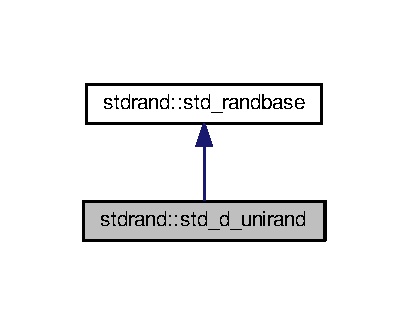
\includegraphics[width=196pt]{de/d88/classstdrand_1_1std__d__unirand__inherit__graph}
\end{center}
\end{figure}


Collaboration diagram for stdrand\+:\+:std\+\_\+d\+\_\+unirand\+:
\nopagebreak
\begin{figure}[H]
\begin{center}
\leavevmode
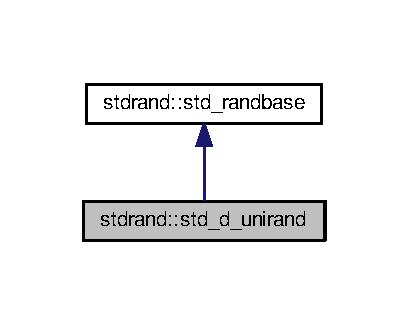
\includegraphics[width=196pt]{d2/dad/classstdrand_1_1std__d__unirand__coll__graph}
\end{center}
\end{figure}
\subsection*{Public Member Functions}
\begin{DoxyCompactItemize}
\item 
\hyperlink{classstdrand_1_1std__d__unirand_aae3235e8e1f6a1d28076899221687273}{std\+\_\+d\+\_\+unirand} (int seed)
\begin{DoxyCompactList}\small\item\em Constructor. \end{DoxyCompactList}\item 
\hyperlink{classstdrand_1_1std__d__unirand_add94ad2a131354549fe22f6f210d8278}{std\+\_\+d\+\_\+unirand} (int size, int seed)
\begin{DoxyCompactList}\small\item\em Constructor with dummy size input. \end{DoxyCompactList}\item 
\hyperlink{classstdrand_1_1std__d__unirand_a37784d8dca5fff875a77224b68cc931b}{$\sim$std\+\_\+d\+\_\+unirand} ()
\begin{DoxyCompactList}\small\item\em Default destructor. \end{DoxyCompactList}\item 
double \hyperlink{classstdrand_1_1std__d__unirand_a3dde71452da1a44bd6be86877e74be74}{gen} ()
\begin{DoxyCompactList}\small\item\em Return a single random number. \end{DoxyCompactList}\end{DoxyCompactItemize}
\subsection*{Additional Inherited Members}


\subsection{Detailed Description}
Generator for uniform numbers between 0 and 1. 

\subsection{Constructor \& Destructor Documentation}
\index{stdrand\+::std\+\_\+d\+\_\+unirand@{stdrand\+::std\+\_\+d\+\_\+unirand}!std\+\_\+d\+\_\+unirand@{std\+\_\+d\+\_\+unirand}}
\index{std\+\_\+d\+\_\+unirand@{std\+\_\+d\+\_\+unirand}!stdrand\+::std\+\_\+d\+\_\+unirand@{stdrand\+::std\+\_\+d\+\_\+unirand}}
\subsubsection[{\texorpdfstring{std\+\_\+d\+\_\+unirand(int seed)}{std_d_unirand(int seed)}}]{\setlength{\rightskip}{0pt plus 5cm}stdrand\+::std\+\_\+d\+\_\+unirand\+::std\+\_\+d\+\_\+unirand (
\begin{DoxyParamCaption}
\item[{int}]{seed}
\end{DoxyParamCaption}
)}\hypertarget{classstdrand_1_1std__d__unirand_aae3235e8e1f6a1d28076899221687273}{}\label{classstdrand_1_1std__d__unirand_aae3235e8e1f6a1d28076899221687273}


Constructor. 


\begin{DoxyParams}{Parameters}
{\em seed} & The inital seed of the random number generator. \\
\hline
\end{DoxyParams}
\index{stdrand\+::std\+\_\+d\+\_\+unirand@{stdrand\+::std\+\_\+d\+\_\+unirand}!std\+\_\+d\+\_\+unirand@{std\+\_\+d\+\_\+unirand}}
\index{std\+\_\+d\+\_\+unirand@{std\+\_\+d\+\_\+unirand}!stdrand\+::std\+\_\+d\+\_\+unirand@{stdrand\+::std\+\_\+d\+\_\+unirand}}
\subsubsection[{\texorpdfstring{std\+\_\+d\+\_\+unirand(int size, int seed)}{std_d_unirand(int size, int seed)}}]{\setlength{\rightskip}{0pt plus 5cm}stdrand\+::std\+\_\+d\+\_\+unirand\+::std\+\_\+d\+\_\+unirand (
\begin{DoxyParamCaption}
\item[{int}]{size, }
\item[{int}]{seed}
\end{DoxyParamCaption}
)\hspace{0.3cm}{\ttfamily [inline]}}\hypertarget{classstdrand_1_1std__d__unirand_add94ad2a131354549fe22f6f210d8278}{}\label{classstdrand_1_1std__d__unirand_add94ad2a131354549fe22f6f210d8278}


Constructor with dummy size input. 


\begin{DoxyParams}{Parameters}
{\em seed} & The inital seed of the random number generator. \\
\hline
{\em size} & A dummy size input for compatibility with Intel R\+NG. \\
\hline
\end{DoxyParams}
\index{stdrand\+::std\+\_\+d\+\_\+unirand@{stdrand\+::std\+\_\+d\+\_\+unirand}!````~std\+\_\+d\+\_\+unirand@{$\sim$std\+\_\+d\+\_\+unirand}}
\index{````~std\+\_\+d\+\_\+unirand@{$\sim$std\+\_\+d\+\_\+unirand}!stdrand\+::std\+\_\+d\+\_\+unirand@{stdrand\+::std\+\_\+d\+\_\+unirand}}
\subsubsection[{\texorpdfstring{$\sim$std\+\_\+d\+\_\+unirand()}{~std_d_unirand()}}]{\setlength{\rightskip}{0pt plus 5cm}stdrand\+::std\+\_\+d\+\_\+unirand\+::$\sim$std\+\_\+d\+\_\+unirand (
\begin{DoxyParamCaption}
{}
\end{DoxyParamCaption}
)\hspace{0.3cm}{\ttfamily [inline]}}\hypertarget{classstdrand_1_1std__d__unirand_a37784d8dca5fff875a77224b68cc931b}{}\label{classstdrand_1_1std__d__unirand_a37784d8dca5fff875a77224b68cc931b}


Default destructor. 



\subsection{Member Function Documentation}
\index{stdrand\+::std\+\_\+d\+\_\+unirand@{stdrand\+::std\+\_\+d\+\_\+unirand}!gen@{gen}}
\index{gen@{gen}!stdrand\+::std\+\_\+d\+\_\+unirand@{stdrand\+::std\+\_\+d\+\_\+unirand}}
\subsubsection[{\texorpdfstring{gen()}{gen()}}]{\setlength{\rightskip}{0pt plus 5cm}double stdrand\+::std\+\_\+d\+\_\+unirand\+::gen (
\begin{DoxyParamCaption}
{}
\end{DoxyParamCaption}
)\hspace{0.3cm}{\ttfamily [inline]}}\hypertarget{classstdrand_1_1std__d__unirand_a3dde71452da1a44bd6be86877e74be74}{}\label{classstdrand_1_1std__d__unirand_a3dde71452da1a44bd6be86877e74be74}


Return a single random number. 



The documentation for this class was generated from the following file\+:\begin{DoxyCompactItemize}
\item 
includes/\hyperlink{stdrand_8hpp}{stdrand.\+hpp}\end{DoxyCompactItemize}

\hypertarget{classstdrand_1_1std__i__unirand}{}\section{stdrand\+:\+:std\+\_\+i\+\_\+unirand Class Reference}
\label{classstdrand_1_1std__i__unirand}\index{stdrand\+::std\+\_\+i\+\_\+unirand@{stdrand\+::std\+\_\+i\+\_\+unirand}}


Generator for uniform integers between 0 and 1.  




{\ttfamily \#include $<$stdrand.\+hpp$>$}



Inheritance diagram for stdrand\+:\+:std\+\_\+i\+\_\+unirand\+:
\nopagebreak
\begin{figure}[H]
\begin{center}
\leavevmode
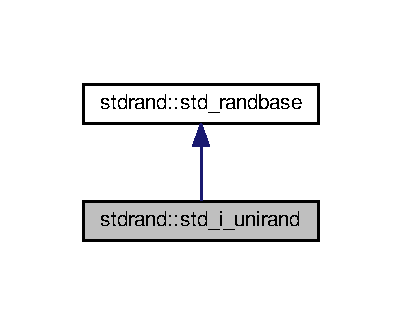
\includegraphics[width=193pt]{d5/d96/classstdrand_1_1std__i__unirand__inherit__graph}
\end{center}
\end{figure}


Collaboration diagram for stdrand\+:\+:std\+\_\+i\+\_\+unirand\+:
\nopagebreak
\begin{figure}[H]
\begin{center}
\leavevmode
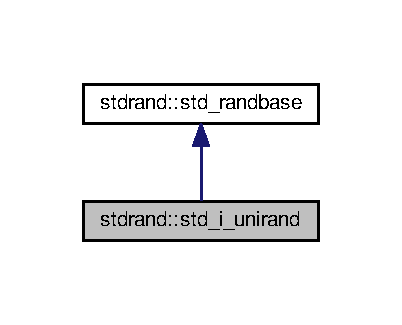
\includegraphics[width=193pt]{d1/d98/classstdrand_1_1std__i__unirand__coll__graph}
\end{center}
\end{figure}
\subsection*{Public Member Functions}
\begin{DoxyCompactItemize}
\item 
\hyperlink{classstdrand_1_1std__i__unirand_a3b8eb8ad27965c98c11d0e62f2f267d6}{std\+\_\+i\+\_\+unirand} (int seed)
\begin{DoxyCompactList}\small\item\em Constructor. \end{DoxyCompactList}\item 
\hyperlink{classstdrand_1_1std__i__unirand_aa43afdb4002553c1d03232e67733de75}{std\+\_\+i\+\_\+unirand} (int size, int seed)
\begin{DoxyCompactList}\small\item\em Constructor with dummy size input. \end{DoxyCompactList}\item 
\hyperlink{classstdrand_1_1std__i__unirand_a1e5b98aecea36f642c829ed5f4e452fc}{$\sim$std\+\_\+i\+\_\+unirand} ()
\begin{DoxyCompactList}\small\item\em Default destructor. \end{DoxyCompactList}\item 
double \hyperlink{classstdrand_1_1std__i__unirand_abe9833ea9fab736cf3b03b529498b767}{gen} ()
\begin{DoxyCompactList}\small\item\em Return a single random number. \end{DoxyCompactList}\end{DoxyCompactItemize}
\subsection*{Additional Inherited Members}


\subsection{Detailed Description}
Generator for uniform integers between 0 and 1. 

\subsection{Constructor \& Destructor Documentation}
\index{stdrand\+::std\+\_\+i\+\_\+unirand@{stdrand\+::std\+\_\+i\+\_\+unirand}!std\+\_\+i\+\_\+unirand@{std\+\_\+i\+\_\+unirand}}
\index{std\+\_\+i\+\_\+unirand@{std\+\_\+i\+\_\+unirand}!stdrand\+::std\+\_\+i\+\_\+unirand@{stdrand\+::std\+\_\+i\+\_\+unirand}}
\subsubsection[{\texorpdfstring{std\+\_\+i\+\_\+unirand(int seed)}{std_i_unirand(int seed)}}]{\setlength{\rightskip}{0pt plus 5cm}stdrand\+::std\+\_\+i\+\_\+unirand\+::std\+\_\+i\+\_\+unirand (
\begin{DoxyParamCaption}
\item[{int}]{seed}
\end{DoxyParamCaption}
)}\hypertarget{classstdrand_1_1std__i__unirand_a3b8eb8ad27965c98c11d0e62f2f267d6}{}\label{classstdrand_1_1std__i__unirand_a3b8eb8ad27965c98c11d0e62f2f267d6}


Constructor. 


\begin{DoxyParams}{Parameters}
{\em seed} & The inital seed of the random number generator. \\
\hline
\end{DoxyParams}
\index{stdrand\+::std\+\_\+i\+\_\+unirand@{stdrand\+::std\+\_\+i\+\_\+unirand}!std\+\_\+i\+\_\+unirand@{std\+\_\+i\+\_\+unirand}}
\index{std\+\_\+i\+\_\+unirand@{std\+\_\+i\+\_\+unirand}!stdrand\+::std\+\_\+i\+\_\+unirand@{stdrand\+::std\+\_\+i\+\_\+unirand}}
\subsubsection[{\texorpdfstring{std\+\_\+i\+\_\+unirand(int size, int seed)}{std_i_unirand(int size, int seed)}}]{\setlength{\rightskip}{0pt plus 5cm}stdrand\+::std\+\_\+i\+\_\+unirand\+::std\+\_\+i\+\_\+unirand (
\begin{DoxyParamCaption}
\item[{int}]{size, }
\item[{int}]{seed}
\end{DoxyParamCaption}
)\hspace{0.3cm}{\ttfamily [inline]}}\hypertarget{classstdrand_1_1std__i__unirand_aa43afdb4002553c1d03232e67733de75}{}\label{classstdrand_1_1std__i__unirand_aa43afdb4002553c1d03232e67733de75}


Constructor with dummy size input. 


\begin{DoxyParams}{Parameters}
{\em seed} & The inital seed of the random number generator. \\
\hline
{\em size} & A dummy size input for compatibility with Intel R\+NG. \\
\hline
\end{DoxyParams}
\index{stdrand\+::std\+\_\+i\+\_\+unirand@{stdrand\+::std\+\_\+i\+\_\+unirand}!````~std\+\_\+i\+\_\+unirand@{$\sim$std\+\_\+i\+\_\+unirand}}
\index{````~std\+\_\+i\+\_\+unirand@{$\sim$std\+\_\+i\+\_\+unirand}!stdrand\+::std\+\_\+i\+\_\+unirand@{stdrand\+::std\+\_\+i\+\_\+unirand}}
\subsubsection[{\texorpdfstring{$\sim$std\+\_\+i\+\_\+unirand()}{~std_i_unirand()}}]{\setlength{\rightskip}{0pt plus 5cm}stdrand\+::std\+\_\+i\+\_\+unirand\+::$\sim$std\+\_\+i\+\_\+unirand (
\begin{DoxyParamCaption}
{}
\end{DoxyParamCaption}
)\hspace{0.3cm}{\ttfamily [inline]}}\hypertarget{classstdrand_1_1std__i__unirand_a1e5b98aecea36f642c829ed5f4e452fc}{}\label{classstdrand_1_1std__i__unirand_a1e5b98aecea36f642c829ed5f4e452fc}


Default destructor. 



\subsection{Member Function Documentation}
\index{stdrand\+::std\+\_\+i\+\_\+unirand@{stdrand\+::std\+\_\+i\+\_\+unirand}!gen@{gen}}
\index{gen@{gen}!stdrand\+::std\+\_\+i\+\_\+unirand@{stdrand\+::std\+\_\+i\+\_\+unirand}}
\subsubsection[{\texorpdfstring{gen()}{gen()}}]{\setlength{\rightskip}{0pt plus 5cm}double stdrand\+::std\+\_\+i\+\_\+unirand\+::gen (
\begin{DoxyParamCaption}
{}
\end{DoxyParamCaption}
)\hspace{0.3cm}{\ttfamily [inline]}}\hypertarget{classstdrand_1_1std__i__unirand_abe9833ea9fab736cf3b03b529498b767}{}\label{classstdrand_1_1std__i__unirand_abe9833ea9fab736cf3b03b529498b767}


Return a single random number. 



The documentation for this class was generated from the following file\+:\begin{DoxyCompactItemize}
\item 
includes/\hyperlink{stdrand_8hpp}{stdrand.\+hpp}\end{DoxyCompactItemize}

\hypertarget{classstdrand_1_1std__lognormrand}{}\section{stdrand\+:\+:std\+\_\+lognormrand Class Reference}
\label{classstdrand_1_1std__lognormrand}\index{stdrand\+::std\+\_\+lognormrand@{stdrand\+::std\+\_\+lognormrand}}


Generator for random numbers on a normal distribution.  




{\ttfamily \#include $<$stdrand.\+hpp$>$}



Inheritance diagram for stdrand\+:\+:std\+\_\+lognormrand\+:
\nopagebreak
\begin{figure}[H]
\begin{center}
\leavevmode
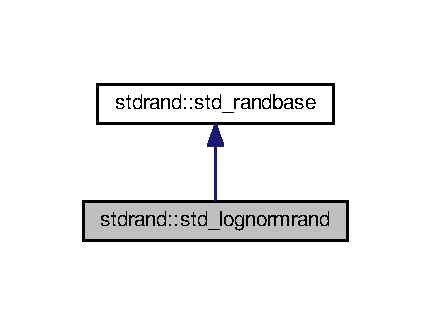
\includegraphics[width=207pt]{d2/deb/classstdrand_1_1std__lognormrand__inherit__graph}
\end{center}
\end{figure}


Collaboration diagram for stdrand\+:\+:std\+\_\+lognormrand\+:
\nopagebreak
\begin{figure}[H]
\begin{center}
\leavevmode
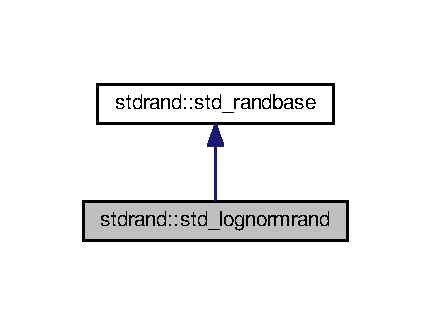
\includegraphics[width=207pt]{d1/d02/classstdrand_1_1std__lognormrand__coll__graph}
\end{center}
\end{figure}
\subsection*{Public Member Functions}
\begin{DoxyCompactItemize}
\item 
\hyperlink{classstdrand_1_1std__lognormrand_a4d27599458dc5b075d723a445431d2f7}{std\+\_\+lognormrand} (double m, double sdin, int seed)
\begin{DoxyCompactList}\small\item\em Constructor. \end{DoxyCompactList}\item 
\hyperlink{classstdrand_1_1std__lognormrand_a21729248c87a39d6522a405a85b6a808}{std\+\_\+lognormrand} (double m, double sdin, int size, int seed)
\begin{DoxyCompactList}\small\item\em Constructor with dummy size. \end{DoxyCompactList}\item 
\hyperlink{classstdrand_1_1std__lognormrand_af73b651b8fde69e3535660eca7fac95f}{$\sim$std\+\_\+lognormrand} ()
\begin{DoxyCompactList}\small\item\em Default destructor. \end{DoxyCompactList}\item 
double \hyperlink{classstdrand_1_1std__lognormrand_a4521bea46b321ea53a2026eac8dc046a}{gen} ()
\begin{DoxyCompactList}\small\item\em Return a single random number. \end{DoxyCompactList}\end{DoxyCompactItemize}
\subsection*{Additional Inherited Members}


\subsection{Detailed Description}
Generator for random numbers on a normal distribution. 

\subsection{Constructor \& Destructor Documentation}
\index{stdrand\+::std\+\_\+lognormrand@{stdrand\+::std\+\_\+lognormrand}!std\+\_\+lognormrand@{std\+\_\+lognormrand}}
\index{std\+\_\+lognormrand@{std\+\_\+lognormrand}!stdrand\+::std\+\_\+lognormrand@{stdrand\+::std\+\_\+lognormrand}}
\subsubsection[{\texorpdfstring{std\+\_\+lognormrand(double m, double sdin, int seed)}{std_lognormrand(double m, double sdin, int seed)}}]{\setlength{\rightskip}{0pt plus 5cm}stdrand\+::std\+\_\+lognormrand\+::std\+\_\+lognormrand (
\begin{DoxyParamCaption}
\item[{double}]{m, }
\item[{double}]{sdin, }
\item[{int}]{seed}
\end{DoxyParamCaption}
)}\hypertarget{classstdrand_1_1std__lognormrand_a4d27599458dc5b075d723a445431d2f7}{}\label{classstdrand_1_1std__lognormrand_a4d27599458dc5b075d723a445431d2f7}


Constructor. 


\begin{DoxyParams}{Parameters}
{\em m} & The logarithmic mean of the lognormal distribution. \\
\hline
{\em sdin} & The logarithmic standard deviation of the lognormal distribution. \\
\hline
{\em seed} & The inital seed of the random number generator. \\
\hline
\end{DoxyParams}
\index{stdrand\+::std\+\_\+lognormrand@{stdrand\+::std\+\_\+lognormrand}!std\+\_\+lognormrand@{std\+\_\+lognormrand}}
\index{std\+\_\+lognormrand@{std\+\_\+lognormrand}!stdrand\+::std\+\_\+lognormrand@{stdrand\+::std\+\_\+lognormrand}}
\subsubsection[{\texorpdfstring{std\+\_\+lognormrand(double m, double sdin, int size, int seed)}{std_lognormrand(double m, double sdin, int size, int seed)}}]{\setlength{\rightskip}{0pt plus 5cm}stdrand\+::std\+\_\+lognormrand\+::std\+\_\+lognormrand (
\begin{DoxyParamCaption}
\item[{double}]{m, }
\item[{double}]{sdin, }
\item[{int}]{size, }
\item[{int}]{seed}
\end{DoxyParamCaption}
)\hspace{0.3cm}{\ttfamily [inline]}}\hypertarget{classstdrand_1_1std__lognormrand_a21729248c87a39d6522a405a85b6a808}{}\label{classstdrand_1_1std__lognormrand_a21729248c87a39d6522a405a85b6a808}


Constructor with dummy size. 


\begin{DoxyParams}{Parameters}
{\em m} & The logarithmic mean of the lognormal distribution. \\
\hline
{\em sdin} & The logarithmic standard deviation of the lognormal distribution. \\
\hline
{\em seed} & The inital seed of the random number generator. \\
\hline
{\em size} & A dummy size input for compatibility with Intel R\+NG. \\
\hline
\end{DoxyParams}
\index{stdrand\+::std\+\_\+lognormrand@{stdrand\+::std\+\_\+lognormrand}!````~std\+\_\+lognormrand@{$\sim$std\+\_\+lognormrand}}
\index{````~std\+\_\+lognormrand@{$\sim$std\+\_\+lognormrand}!stdrand\+::std\+\_\+lognormrand@{stdrand\+::std\+\_\+lognormrand}}
\subsubsection[{\texorpdfstring{$\sim$std\+\_\+lognormrand()}{~std_lognormrand()}}]{\setlength{\rightskip}{0pt plus 5cm}stdrand\+::std\+\_\+lognormrand\+::$\sim$std\+\_\+lognormrand (
\begin{DoxyParamCaption}
{}
\end{DoxyParamCaption}
)\hspace{0.3cm}{\ttfamily [inline]}}\hypertarget{classstdrand_1_1std__lognormrand_af73b651b8fde69e3535660eca7fac95f}{}\label{classstdrand_1_1std__lognormrand_af73b651b8fde69e3535660eca7fac95f}


Default destructor. 



\subsection{Member Function Documentation}
\index{stdrand\+::std\+\_\+lognormrand@{stdrand\+::std\+\_\+lognormrand}!gen@{gen}}
\index{gen@{gen}!stdrand\+::std\+\_\+lognormrand@{stdrand\+::std\+\_\+lognormrand}}
\subsubsection[{\texorpdfstring{gen()}{gen()}}]{\setlength{\rightskip}{0pt plus 5cm}double stdrand\+::std\+\_\+lognormrand\+::gen (
\begin{DoxyParamCaption}
{}
\end{DoxyParamCaption}
)\hspace{0.3cm}{\ttfamily [inline]}}\hypertarget{classstdrand_1_1std__lognormrand_a4521bea46b321ea53a2026eac8dc046a}{}\label{classstdrand_1_1std__lognormrand_a4521bea46b321ea53a2026eac8dc046a}


Return a single random number. 



The documentation for this class was generated from the following file\+:\begin{DoxyCompactItemize}
\item 
includes/\hyperlink{stdrand_8hpp}{stdrand.\+hpp}\end{DoxyCompactItemize}

\hypertarget{classstdrand_1_1std__normrand}{}\section{stdrand\+:\+:std\+\_\+normrand Class Reference}
\label{classstdrand_1_1std__normrand}\index{stdrand\+::std\+\_\+normrand@{stdrand\+::std\+\_\+normrand}}


Generator for random numbers on a normal distribution.  




{\ttfamily \#include $<$stdrand.\+hpp$>$}



Inheritance diagram for stdrand\+:\+:std\+\_\+normrand\+:
\nopagebreak
\begin{figure}[H]
\begin{center}
\leavevmode
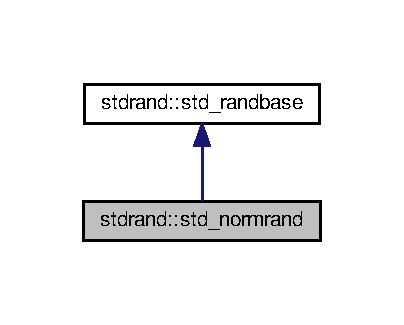
\includegraphics[width=194pt]{d0/df7/classstdrand_1_1std__normrand__inherit__graph}
\end{center}
\end{figure}


Collaboration diagram for stdrand\+:\+:std\+\_\+normrand\+:
\nopagebreak
\begin{figure}[H]
\begin{center}
\leavevmode
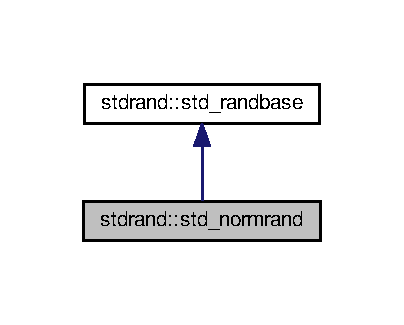
\includegraphics[width=194pt]{d6/d3d/classstdrand_1_1std__normrand__coll__graph}
\end{center}
\end{figure}
\subsection*{Public Member Functions}
\begin{DoxyCompactItemize}
\item 
\hyperlink{classstdrand_1_1std__normrand_a2cb06e8547d4475a424d213cda700ad7}{std\+\_\+normrand} (double m, double sdin, int seed=1)
\begin{DoxyCompactList}\small\item\em Constructor. \end{DoxyCompactList}\item 
\hyperlink{classstdrand_1_1std__normrand_aec1727d2023b6acc65a4057a71ee642a}{$\sim$std\+\_\+normrand} ()
\begin{DoxyCompactList}\small\item\em Default destructor. \end{DoxyCompactList}\item 
double \hyperlink{classstdrand_1_1std__normrand_adf3d7e53ddd7a0aa6b43b08038f09c91}{gen} ()
\begin{DoxyCompactList}\small\item\em Return a single random number. \end{DoxyCompactList}\end{DoxyCompactItemize}
\subsection*{Additional Inherited Members}


\subsection{Detailed Description}
Generator for random numbers on a normal distribution. 

\subsection{Constructor \& Destructor Documentation}
\index{stdrand\+::std\+\_\+normrand@{stdrand\+::std\+\_\+normrand}!std\+\_\+normrand@{std\+\_\+normrand}}
\index{std\+\_\+normrand@{std\+\_\+normrand}!stdrand\+::std\+\_\+normrand@{stdrand\+::std\+\_\+normrand}}
\subsubsection[{\texorpdfstring{std\+\_\+normrand(double m, double sdin, int seed=1)}{std_normrand(double m, double sdin, int seed=1)}}]{\setlength{\rightskip}{0pt plus 5cm}stdrand\+::std\+\_\+normrand\+::std\+\_\+normrand (
\begin{DoxyParamCaption}
\item[{double}]{m, }
\item[{double}]{sdin, }
\item[{int}]{seed = {\ttfamily 1}}
\end{DoxyParamCaption}
)}\hypertarget{classstdrand_1_1std__normrand_a2cb06e8547d4475a424d213cda700ad7}{}\label{classstdrand_1_1std__normrand_a2cb06e8547d4475a424d213cda700ad7}


Constructor. 


\begin{DoxyParams}{Parameters}
{\em m} & The mean of the normal distribution. \\
\hline
{\em sdin} & The standard deviation of the normal distribution. \\
\hline
{\em seed} & The inital seed of the random number generator. Defaults to 1. \\
\hline
\end{DoxyParams}
\index{stdrand\+::std\+\_\+normrand@{stdrand\+::std\+\_\+normrand}!````~std\+\_\+normrand@{$\sim$std\+\_\+normrand}}
\index{````~std\+\_\+normrand@{$\sim$std\+\_\+normrand}!stdrand\+::std\+\_\+normrand@{stdrand\+::std\+\_\+normrand}}
\subsubsection[{\texorpdfstring{$\sim$std\+\_\+normrand()}{~std_normrand()}}]{\setlength{\rightskip}{0pt plus 5cm}stdrand\+::std\+\_\+normrand\+::$\sim$std\+\_\+normrand (
\begin{DoxyParamCaption}
{}
\end{DoxyParamCaption}
)\hspace{0.3cm}{\ttfamily [inline]}}\hypertarget{classstdrand_1_1std__normrand_aec1727d2023b6acc65a4057a71ee642a}{}\label{classstdrand_1_1std__normrand_aec1727d2023b6acc65a4057a71ee642a}


Default destructor. 



\subsection{Member Function Documentation}
\index{stdrand\+::std\+\_\+normrand@{stdrand\+::std\+\_\+normrand}!gen@{gen}}
\index{gen@{gen}!stdrand\+::std\+\_\+normrand@{stdrand\+::std\+\_\+normrand}}
\subsubsection[{\texorpdfstring{gen()}{gen()}}]{\setlength{\rightskip}{0pt plus 5cm}double stdrand\+::std\+\_\+normrand\+::gen (
\begin{DoxyParamCaption}
{}
\end{DoxyParamCaption}
)\hspace{0.3cm}{\ttfamily [inline]}}\hypertarget{classstdrand_1_1std__normrand_adf3d7e53ddd7a0aa6b43b08038f09c91}{}\label{classstdrand_1_1std__normrand_adf3d7e53ddd7a0aa6b43b08038f09c91}


Return a single random number. 



The documentation for this class was generated from the following file\+:\begin{DoxyCompactItemize}
\item 
includes/\hyperlink{stdrand_8hpp}{stdrand.\+hpp}\end{DoxyCompactItemize}

\hypertarget{classstdrand_1_1std__randbase}{}\section{stdrand\+:\+:std\+\_\+randbase Class Reference}
\label{classstdrand_1_1std__randbase}\index{stdrand\+::std\+\_\+randbase@{stdrand\+::std\+\_\+randbase}}


Base class for the random number generators.  




{\ttfamily \#include $<$stdrand.\+hpp$>$}



Inheritance diagram for stdrand\+:\+:std\+\_\+randbase\+:\nopagebreak
\begin{figure}[H]
\begin{center}
\leavevmode
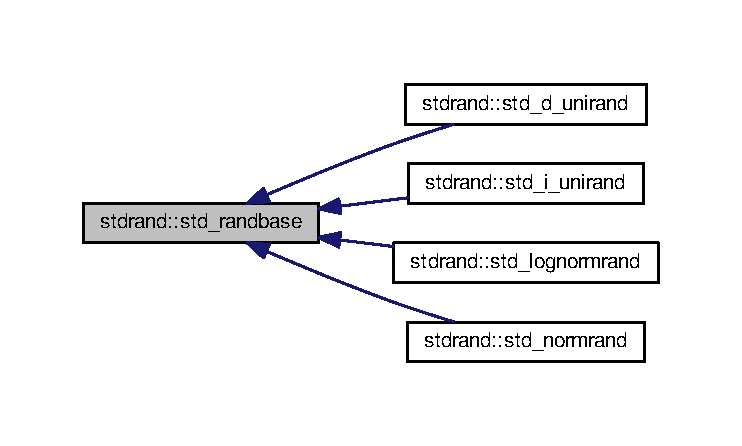
\includegraphics[width=350pt]{d1/d27/classstdrand_1_1std__randbase__inherit__graph}
\end{center}
\end{figure}


Collaboration diagram for stdrand\+:\+:std\+\_\+randbase\+:
\nopagebreak
\begin{figure}[H]
\begin{center}
\leavevmode
\includegraphics[width=193pt]{d0/d37/classstdrand_1_1std__randbase__coll__graph}
\end{center}
\end{figure}
\subsection*{Public Member Functions}
\begin{DoxyCompactItemize}
\item 
\hyperlink{classstdrand_1_1std__randbase_a8298d43186d6410f30ec0a77f0b90159}{std\+\_\+randbase} ()
\begin{DoxyCompactList}\small\item\em Default constructor. \end{DoxyCompactList}\item 
\hyperlink{classstdrand_1_1std__randbase_a5280080005689ab2ff6dae6de10a3faa}{$\sim$std\+\_\+randbase} ()
\begin{DoxyCompactList}\small\item\em Default destructor. \end{DoxyCompactList}\item 
void \hyperlink{classstdrand_1_1std__randbase_ae4d2a7ab5253b8d21ce4ede8f9988f24}{change\+\_\+seed} (int seed)
\begin{DoxyCompactList}\small\item\em Change the current random seed. \end{DoxyCompactList}\item 
void \hyperlink{classstdrand_1_1std__randbase_a1f59d641467d33c51df65651212dac1f}{jump} ()
\begin{DoxyCompactList}\small\item\em Jump forward 2$^\wedge$64 places. \end{DoxyCompactList}\end{DoxyCompactItemize}
\subsection*{Protected Attributes}
\begin{DoxyCompactItemize}
\item 
\hyperlink{structrng_1_1rng128}{rng\+::rng128} \hyperlink{classstdrand_1_1std__randbase_a04dc8f49595791e10967b74a4b137b53}{generator}
\end{DoxyCompactItemize}


\subsection{Detailed Description}
Base class for the random number generators. 

\subsection{Constructor \& Destructor Documentation}
\index{stdrand\+::std\+\_\+randbase@{stdrand\+::std\+\_\+randbase}!std\+\_\+randbase@{std\+\_\+randbase}}
\index{std\+\_\+randbase@{std\+\_\+randbase}!stdrand\+::std\+\_\+randbase@{stdrand\+::std\+\_\+randbase}}
\subsubsection[{\texorpdfstring{std\+\_\+randbase()}{std_randbase()}}]{\setlength{\rightskip}{0pt plus 5cm}stdrand\+::std\+\_\+randbase\+::std\+\_\+randbase (
\begin{DoxyParamCaption}
{}
\end{DoxyParamCaption}
)\hspace{0.3cm}{\ttfamily [inline]}}\hypertarget{classstdrand_1_1std__randbase_a8298d43186d6410f30ec0a77f0b90159}{}\label{classstdrand_1_1std__randbase_a8298d43186d6410f30ec0a77f0b90159}


Default constructor. 

\index{stdrand\+::std\+\_\+randbase@{stdrand\+::std\+\_\+randbase}!````~std\+\_\+randbase@{$\sim$std\+\_\+randbase}}
\index{````~std\+\_\+randbase@{$\sim$std\+\_\+randbase}!stdrand\+::std\+\_\+randbase@{stdrand\+::std\+\_\+randbase}}
\subsubsection[{\texorpdfstring{$\sim$std\+\_\+randbase()}{~std_randbase()}}]{\setlength{\rightskip}{0pt plus 5cm}stdrand\+::std\+\_\+randbase\+::$\sim$std\+\_\+randbase (
\begin{DoxyParamCaption}
{}
\end{DoxyParamCaption}
)\hspace{0.3cm}{\ttfamily [inline]}}\hypertarget{classstdrand_1_1std__randbase_a5280080005689ab2ff6dae6de10a3faa}{}\label{classstdrand_1_1std__randbase_a5280080005689ab2ff6dae6de10a3faa}


Default destructor. 



\subsection{Member Function Documentation}
\index{stdrand\+::std\+\_\+randbase@{stdrand\+::std\+\_\+randbase}!change\+\_\+seed@{change\+\_\+seed}}
\index{change\+\_\+seed@{change\+\_\+seed}!stdrand\+::std\+\_\+randbase@{stdrand\+::std\+\_\+randbase}}
\subsubsection[{\texorpdfstring{change\+\_\+seed(int seed)}{change_seed(int seed)}}]{\setlength{\rightskip}{0pt plus 5cm}void stdrand\+::std\+\_\+randbase\+::change\+\_\+seed (
\begin{DoxyParamCaption}
\item[{int}]{seed}
\end{DoxyParamCaption}
)\hspace{0.3cm}{\ttfamily [inline]}}\hypertarget{classstdrand_1_1std__randbase_ae4d2a7ab5253b8d21ce4ede8f9988f24}{}\label{classstdrand_1_1std__randbase_ae4d2a7ab5253b8d21ce4ede8f9988f24}


Change the current random seed. 


\begin{DoxyParams}{Parameters}
{\em seed} & The new seed. \\
\hline
\end{DoxyParams}
\index{stdrand\+::std\+\_\+randbase@{stdrand\+::std\+\_\+randbase}!jump@{jump}}
\index{jump@{jump}!stdrand\+::std\+\_\+randbase@{stdrand\+::std\+\_\+randbase}}
\subsubsection[{\texorpdfstring{jump()}{jump()}}]{\setlength{\rightskip}{0pt plus 5cm}void stdrand\+::std\+\_\+randbase\+::jump (
\begin{DoxyParamCaption}
{}
\end{DoxyParamCaption}
)\hspace{0.3cm}{\ttfamily [inline]}}\hypertarget{classstdrand_1_1std__randbase_a1f59d641467d33c51df65651212dac1f}{}\label{classstdrand_1_1std__randbase_a1f59d641467d33c51df65651212dac1f}


Jump forward 2$^\wedge$64 places. 



\subsection{Member Data Documentation}
\index{stdrand\+::std\+\_\+randbase@{stdrand\+::std\+\_\+randbase}!generator@{generator}}
\index{generator@{generator}!stdrand\+::std\+\_\+randbase@{stdrand\+::std\+\_\+randbase}}
\subsubsection[{\texorpdfstring{generator}{generator}}]{\setlength{\rightskip}{0pt plus 5cm}{\bf rng\+::rng128} stdrand\+::std\+\_\+randbase\+::generator\hspace{0.3cm}{\ttfamily [protected]}}\hypertarget{classstdrand_1_1std__randbase_a04dc8f49595791e10967b74a4b137b53}{}\label{classstdrand_1_1std__randbase_a04dc8f49595791e10967b74a4b137b53}


The documentation for this class was generated from the following file\+:\begin{DoxyCompactItemize}
\item 
includes/\hyperlink{stdrand_8hpp}{stdrand.\+hpp}\end{DoxyCompactItemize}

\hypertarget{structrng_1_1tsc__seed}{}\section{rng\+:\+:tsc\+\_\+seed Struct Reference}
\label{structrng_1_1tsc__seed}\index{rng\+::tsc\+\_\+seed@{rng\+::tsc\+\_\+seed}}


{\ttfamily \#include $<$xoroshiro128.\+hpp$>$}

\subsection*{Public Types}
\begin{DoxyCompactItemize}
\item 
using \hyperlink{structrng_1_1tsc__seed_a05c16f9b935c21f149451c12ddb31d16}{result\+\_\+type} = std\+::uint64\+\_\+t
\end{DoxyCompactItemize}
\subsection*{Public Member Functions}
\begin{DoxyCompactItemize}
\item 
\hyperlink{structrng_1_1tsc__seed_a05c16f9b935c21f149451c12ddb31d16}{result\+\_\+type} \hyperlink{structrng_1_1tsc__seed_a55949da9d3b5acb54f0f87e1707c3c73}{operator()} ()
\end{DoxyCompactItemize}


\subsection{Member Typedef Documentation}
\index{rng\+::tsc\+\_\+seed@{rng\+::tsc\+\_\+seed}!result\+\_\+type@{result\+\_\+type}}
\index{result\+\_\+type@{result\+\_\+type}!rng\+::tsc\+\_\+seed@{rng\+::tsc\+\_\+seed}}
\subsubsection[{\texorpdfstring{result\+\_\+type}{result_type}}]{\setlength{\rightskip}{0pt plus 5cm}using {\bf rng\+::tsc\+\_\+seed\+::result\+\_\+type} =  std\+::uint64\+\_\+t}\hypertarget{structrng_1_1tsc__seed_a05c16f9b935c21f149451c12ddb31d16}{}\label{structrng_1_1tsc__seed_a05c16f9b935c21f149451c12ddb31d16}


\subsection{Member Function Documentation}
\index{rng\+::tsc\+\_\+seed@{rng\+::tsc\+\_\+seed}!operator()@{operator()}}
\index{operator()@{operator()}!rng\+::tsc\+\_\+seed@{rng\+::tsc\+\_\+seed}}
\subsubsection[{\texorpdfstring{operator()()}{operator()()}}]{\setlength{\rightskip}{0pt plus 5cm}{\bf result\+\_\+type} rng\+::tsc\+\_\+seed\+::operator() (
\begin{DoxyParamCaption}
{}
\end{DoxyParamCaption}
)\hspace{0.3cm}{\ttfamily [inline]}}\hypertarget{structrng_1_1tsc__seed_a55949da9d3b5acb54f0f87e1707c3c73}{}\label{structrng_1_1tsc__seed_a55949da9d3b5acb54f0f87e1707c3c73}


The documentation for this struct was generated from the following file\+:\begin{DoxyCompactItemize}
\item 
includes/\hyperlink{xoroshiro128_8hpp}{xoroshiro128.\+hpp}\end{DoxyCompactItemize}

\hypertarget{classparticle_1_1shape_1_1weibull}{}\section{particle\+:\+:shape\+:\+:weibull Class Reference}
\label{classparticle_1_1shape_1_1weibull}\index{particle\+::shape\+::weibull@{particle\+::shape\+::weibull}}


Weibull disordered circle/sphere particle.  




{\ttfamily \#include $<$shape.\+hpp$>$}



Inheritance diagram for particle\+:\+:shape\+:\+:weibull\+:\nopagebreak
\begin{figure}[H]
\begin{center}
\leavevmode
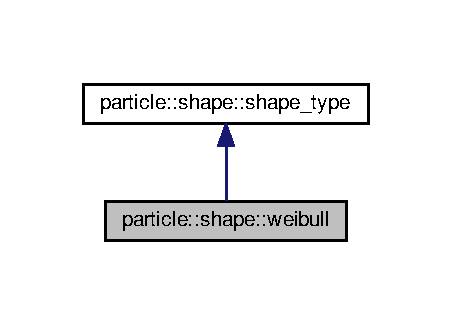
\includegraphics[width=217pt]{dc/d64/classparticle_1_1shape_1_1weibull__inherit__graph}
\end{center}
\end{figure}


Collaboration diagram for particle\+:\+:shape\+:\+:weibull\+:\nopagebreak
\begin{figure}[H]
\begin{center}
\leavevmode
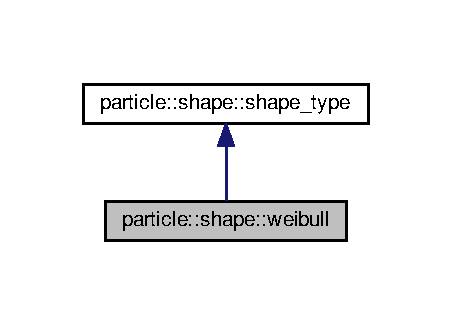
\includegraphics[width=217pt]{dd/d57/classparticle_1_1shape_1_1weibull__coll__graph}
\end{center}
\end{figure}
\subsection*{Public Member Functions}
\begin{DoxyCompactItemize}
\item 
\hyperlink{classparticle_1_1shape_1_1weibull_a6171e8485c445df5322b61bc4bd4d360}{weibull} ()
\begin{DoxyCompactList}\small\item\em Default constructor. \end{DoxyCompactList}\item 
\hyperlink{classparticle_1_1shape_1_1weibull_a4a30c2bc444fddc10e53331693b1b696}{weibull} (\hyperlink{classparticle_1_1shape_1_1shape__type}{shape\+\_\+type} \&other)
\begin{DoxyCompactList}\small\item\em Copy constructor. \end{DoxyCompactList}\item 
\hyperlink{classparticle_1_1shape_1_1weibull_ae3ea5c72d6cb62ba72308ed831bbc82d}{weibull} (double rin, double bin)
\begin{DoxyCompactList}\small\item\em Constructor defining a spherical particle with a disordered surface. \end{DoxyCompactList}\item 
\hyperlink{classparticle_1_1shape_1_1weibull_a63137884cacc8ab5df125ba862f79262}{weibull} (double betain, double ain, double bin, double cin)
\begin{DoxyCompactList}\small\item\em Constructor defining an ellipsoid particle with a disordered surface. \end{DoxyCompactList}\item 
\hyperlink{classparticle_1_1shape_1_1weibull_a02613f15cab64462293ff787c35fafb1}{$\sim$weibull} ()
\begin{DoxyCompactList}\small\item\em Default destructor. \end{DoxyCompactList}\item 
bool \hyperlink{classparticle_1_1shape_1_1weibull_a22612311ce2f3ca4317f8263e52de425}{check} (std\+::vector$<$ int $>$ Is, int l\+\_\+size)
\begin{DoxyCompactList}\small\item\em Check whether a certain position falls within the particle. \end{DoxyCompactList}\item 
\hyperlink{classparticle_1_1shape_1_1weibull}{weibull} \& \hyperlink{classparticle_1_1shape_1_1weibull_a682194c48696724e2290373b8c35577a}{operator=} (\hyperlink{classparticle_1_1shape_1_1shape__type}{shape\+\_\+type} \&other)
\begin{DoxyCompactList}\small\item\em Assignment operator. \end{DoxyCompactList}\item 
double \hyperlink{classparticle_1_1shape_1_1weibull_a85ab45f804ae9aa3fb712c435125ff70}{get\+\_\+r0} ()
\begin{DoxyCompactList}\small\item\em Returns the characteristic size of a weibull particle. \end{DoxyCompactList}\item 
double \hyperlink{classparticle_1_1shape_1_1weibull_a640180ce2bd6ce7f68c10d4791bce49c}{get\+\_\+beta} ()
\begin{DoxyCompactList}\small\item\em Returns the disorder parameter of a weibull particle. \end{DoxyCompactList}\item 
double \hyperlink{classparticle_1_1shape_1_1weibull_a0234fa42b67465c7191248f524f27a0e}{get\+\_\+a} ()
\begin{DoxyCompactList}\small\item\em Returns the x-\/axis radius of a weibull particle. \end{DoxyCompactList}\item 
double \hyperlink{classparticle_1_1shape_1_1weibull_a1066adcab828f8636475128ff51c56f0}{get\+\_\+b} ()
\begin{DoxyCompactList}\small\item\em Returns the y-\/axis radius of a weibull particle. \end{DoxyCompactList}\item 
double \hyperlink{classparticle_1_1shape_1_1weibull_a0b8c38944e502df7bce4e8f99d149237}{get\+\_\+c} ()
\begin{DoxyCompactList}\small\item\em Returns the z-\/axis radius of a weibull particle. \end{DoxyCompactList}\end{DoxyCompactItemize}


\subsection{Detailed Description}
Weibull disordered circle/sphere particle. 

\subsection{Constructor \& Destructor Documentation}
\index{particle\+::shape\+::weibull@{particle\+::shape\+::weibull}!weibull@{weibull}}
\index{weibull@{weibull}!particle\+::shape\+::weibull@{particle\+::shape\+::weibull}}
\subsubsection[{\texorpdfstring{weibull()}{weibull()}}]{\setlength{\rightskip}{0pt plus 5cm}particle\+::shape\+::weibull\+::weibull (
\begin{DoxyParamCaption}
{}
\end{DoxyParamCaption}
)\hspace{0.3cm}{\ttfamily [inline]}}\hypertarget{classparticle_1_1shape_1_1weibull_a6171e8485c445df5322b61bc4bd4d360}{}\label{classparticle_1_1shape_1_1weibull_a6171e8485c445df5322b61bc4bd4d360}


Default constructor. 

\index{particle\+::shape\+::weibull@{particle\+::shape\+::weibull}!weibull@{weibull}}
\index{weibull@{weibull}!particle\+::shape\+::weibull@{particle\+::shape\+::weibull}}
\subsubsection[{\texorpdfstring{weibull(shape\+\_\+type \&other)}{weibull(shape_type &other)}}]{\setlength{\rightskip}{0pt plus 5cm}particle\+::shape\+::weibull\+::weibull (
\begin{DoxyParamCaption}
\item[{{\bf shape\+\_\+type} \&}]{other}
\end{DoxyParamCaption}
)}\hypertarget{classparticle_1_1shape_1_1weibull_a4a30c2bc444fddc10e53331693b1b696}{}\label{classparticle_1_1shape_1_1weibull_a4a30c2bc444fddc10e53331693b1b696}


Copy constructor. 

\index{particle\+::shape\+::weibull@{particle\+::shape\+::weibull}!weibull@{weibull}}
\index{weibull@{weibull}!particle\+::shape\+::weibull@{particle\+::shape\+::weibull}}
\subsubsection[{\texorpdfstring{weibull(double rin, double bin)}{weibull(double rin, double bin)}}]{\setlength{\rightskip}{0pt plus 5cm}particle\+::shape\+::weibull\+::weibull (
\begin{DoxyParamCaption}
\item[{double}]{rin, }
\item[{double}]{bin}
\end{DoxyParamCaption}
)}\hypertarget{classparticle_1_1shape_1_1weibull_ae3ea5c72d6cb62ba72308ed831bbc82d}{}\label{classparticle_1_1shape_1_1weibull_ae3ea5c72d6cb62ba72308ed831bbc82d}


Constructor defining a spherical particle with a disordered surface. 


\begin{DoxyParams}{Parameters}
{\em rin} & The average radius of the sphere. \\
\hline
{\em bin} & The disorder parameter. \\
\hline
\end{DoxyParams}
\index{particle\+::shape\+::weibull@{particle\+::shape\+::weibull}!weibull@{weibull}}
\index{weibull@{weibull}!particle\+::shape\+::weibull@{particle\+::shape\+::weibull}}
\subsubsection[{\texorpdfstring{weibull(double betain, double ain, double bin, double cin)}{weibull(double betain, double ain, double bin, double cin)}}]{\setlength{\rightskip}{0pt plus 5cm}particle\+::shape\+::weibull\+::weibull (
\begin{DoxyParamCaption}
\item[{double}]{betain, }
\item[{double}]{ain, }
\item[{double}]{bin, }
\item[{double}]{cin}
\end{DoxyParamCaption}
)}\hypertarget{classparticle_1_1shape_1_1weibull_a63137884cacc8ab5df125ba862f79262}{}\label{classparticle_1_1shape_1_1weibull_a63137884cacc8ab5df125ba862f79262}


Constructor defining an ellipsoid particle with a disordered surface. 


\begin{DoxyParams}{Parameters}
{\em betain} & The disorder parameter. \\
\hline
{\em ain} & The x-\/axis size of the particle. \\
\hline
{\em bin} & The y-\/axis size of the particle. \\
\hline
{\em cin} & The z-\/axis size of the particle. \\
\hline
\end{DoxyParams}
\index{particle\+::shape\+::weibull@{particle\+::shape\+::weibull}!````~weibull@{$\sim$weibull}}
\index{````~weibull@{$\sim$weibull}!particle\+::shape\+::weibull@{particle\+::shape\+::weibull}}
\subsubsection[{\texorpdfstring{$\sim$weibull()}{~weibull()}}]{\setlength{\rightskip}{0pt plus 5cm}particle\+::shape\+::weibull\+::$\sim$weibull (
\begin{DoxyParamCaption}
{}
\end{DoxyParamCaption}
)\hspace{0.3cm}{\ttfamily [inline]}}\hypertarget{classparticle_1_1shape_1_1weibull_a02613f15cab64462293ff787c35fafb1}{}\label{classparticle_1_1shape_1_1weibull_a02613f15cab64462293ff787c35fafb1}


Default destructor. 



\subsection{Member Function Documentation}
\index{particle\+::shape\+::weibull@{particle\+::shape\+::weibull}!check@{check}}
\index{check@{check}!particle\+::shape\+::weibull@{particle\+::shape\+::weibull}}
\subsubsection[{\texorpdfstring{check(std\+::vector$<$ int $>$ Is, int l\+\_\+size)}{check(std::vector< int > Is, int l_size)}}]{\setlength{\rightskip}{0pt plus 5cm}bool particle\+::shape\+::weibull\+::check (
\begin{DoxyParamCaption}
\item[{std\+::vector$<$ int $>$}]{Is, }
\item[{int}]{l\+\_\+size}
\end{DoxyParamCaption}
)\hspace{0.3cm}{\ttfamily [virtual]}}\hypertarget{classparticle_1_1shape_1_1weibull_a22612311ce2f3ca4317f8263e52de425}{}\label{classparticle_1_1shape_1_1weibull_a22612311ce2f3ca4317f8263e52de425}


Check whether a certain position falls within the particle. 


\begin{DoxyParams}{Parameters}
{\em Is} & The coordinates of the lattice site. \\
\hline
{\em l\+\_\+size} & The total lattice size. \\
\hline
\end{DoxyParams}


Reimplemented from \hyperlink{classparticle_1_1shape_1_1shape__type_a64d04f49c8da656d8b8899c431c346fc}{particle\+::shape\+::shape\+\_\+type}.

\index{particle\+::shape\+::weibull@{particle\+::shape\+::weibull}!get\+\_\+a@{get\+\_\+a}}
\index{get\+\_\+a@{get\+\_\+a}!particle\+::shape\+::weibull@{particle\+::shape\+::weibull}}
\subsubsection[{\texorpdfstring{get\+\_\+a()}{get_a()}}]{\setlength{\rightskip}{0pt plus 5cm}double particle\+::shape\+::weibull\+::get\+\_\+a (
\begin{DoxyParamCaption}
{}
\end{DoxyParamCaption}
)\hspace{0.3cm}{\ttfamily [inline]}, {\ttfamily [virtual]}}\hypertarget{classparticle_1_1shape_1_1weibull_a0234fa42b67465c7191248f524f27a0e}{}\label{classparticle_1_1shape_1_1weibull_a0234fa42b67465c7191248f524f27a0e}


Returns the x-\/axis radius of a weibull particle. 



Reimplemented from \hyperlink{classparticle_1_1shape_1_1shape__type_a7b938aa8c2dada71e8d0b11c6a676449}{particle\+::shape\+::shape\+\_\+type}.

\index{particle\+::shape\+::weibull@{particle\+::shape\+::weibull}!get\+\_\+b@{get\+\_\+b}}
\index{get\+\_\+b@{get\+\_\+b}!particle\+::shape\+::weibull@{particle\+::shape\+::weibull}}
\subsubsection[{\texorpdfstring{get\+\_\+b()}{get_b()}}]{\setlength{\rightskip}{0pt plus 5cm}double particle\+::shape\+::weibull\+::get\+\_\+b (
\begin{DoxyParamCaption}
{}
\end{DoxyParamCaption}
)\hspace{0.3cm}{\ttfamily [inline]}, {\ttfamily [virtual]}}\hypertarget{classparticle_1_1shape_1_1weibull_a1066adcab828f8636475128ff51c56f0}{}\label{classparticle_1_1shape_1_1weibull_a1066adcab828f8636475128ff51c56f0}


Returns the y-\/axis radius of a weibull particle. 



Reimplemented from \hyperlink{classparticle_1_1shape_1_1shape__type_a0a9f0a397edbc66120114c89a185c127}{particle\+::shape\+::shape\+\_\+type}.

\index{particle\+::shape\+::weibull@{particle\+::shape\+::weibull}!get\+\_\+beta@{get\+\_\+beta}}
\index{get\+\_\+beta@{get\+\_\+beta}!particle\+::shape\+::weibull@{particle\+::shape\+::weibull}}
\subsubsection[{\texorpdfstring{get\+\_\+beta()}{get_beta()}}]{\setlength{\rightskip}{0pt plus 5cm}double particle\+::shape\+::weibull\+::get\+\_\+beta (
\begin{DoxyParamCaption}
{}
\end{DoxyParamCaption}
)\hspace{0.3cm}{\ttfamily [inline]}, {\ttfamily [virtual]}}\hypertarget{classparticle_1_1shape_1_1weibull_a640180ce2bd6ce7f68c10d4791bce49c}{}\label{classparticle_1_1shape_1_1weibull_a640180ce2bd6ce7f68c10d4791bce49c}


Returns the disorder parameter of a weibull particle. 



Reimplemented from \hyperlink{classparticle_1_1shape_1_1shape__type_a041dd08774f26ffeeb051e1442cb612c}{particle\+::shape\+::shape\+\_\+type}.

\index{particle\+::shape\+::weibull@{particle\+::shape\+::weibull}!get\+\_\+c@{get\+\_\+c}}
\index{get\+\_\+c@{get\+\_\+c}!particle\+::shape\+::weibull@{particle\+::shape\+::weibull}}
\subsubsection[{\texorpdfstring{get\+\_\+c()}{get_c()}}]{\setlength{\rightskip}{0pt plus 5cm}double particle\+::shape\+::weibull\+::get\+\_\+c (
\begin{DoxyParamCaption}
{}
\end{DoxyParamCaption}
)\hspace{0.3cm}{\ttfamily [inline]}, {\ttfamily [virtual]}}\hypertarget{classparticle_1_1shape_1_1weibull_a0b8c38944e502df7bce4e8f99d149237}{}\label{classparticle_1_1shape_1_1weibull_a0b8c38944e502df7bce4e8f99d149237}


Returns the z-\/axis radius of a weibull particle. 



Reimplemented from \hyperlink{classparticle_1_1shape_1_1shape__type_a4f37d43b6e014a429e45480cea48f63d}{particle\+::shape\+::shape\+\_\+type}.

\index{particle\+::shape\+::weibull@{particle\+::shape\+::weibull}!get\+\_\+r0@{get\+\_\+r0}}
\index{get\+\_\+r0@{get\+\_\+r0}!particle\+::shape\+::weibull@{particle\+::shape\+::weibull}}
\subsubsection[{\texorpdfstring{get\+\_\+r0()}{get_r0()}}]{\setlength{\rightskip}{0pt plus 5cm}double particle\+::shape\+::weibull\+::get\+\_\+r0 (
\begin{DoxyParamCaption}
{}
\end{DoxyParamCaption}
)\hspace{0.3cm}{\ttfamily [inline]}, {\ttfamily [virtual]}}\hypertarget{classparticle_1_1shape_1_1weibull_a85ab45f804ae9aa3fb712c435125ff70}{}\label{classparticle_1_1shape_1_1weibull_a85ab45f804ae9aa3fb712c435125ff70}


Returns the characteristic size of a weibull particle. 



Reimplemented from \hyperlink{classparticle_1_1shape_1_1shape__type_a062dfaf9cbfe98cdcdc55c34a0463313}{particle\+::shape\+::shape\+\_\+type}.

\index{particle\+::shape\+::weibull@{particle\+::shape\+::weibull}!operator=@{operator=}}
\index{operator=@{operator=}!particle\+::shape\+::weibull@{particle\+::shape\+::weibull}}
\subsubsection[{\texorpdfstring{operator=(shape\+\_\+type \&other)}{operator=(shape_type &other)}}]{\setlength{\rightskip}{0pt plus 5cm}{\bf weibull}\& particle\+::shape\+::weibull\+::operator= (
\begin{DoxyParamCaption}
\item[{{\bf shape\+\_\+type} \&}]{other}
\end{DoxyParamCaption}
)}\hypertarget{classparticle_1_1shape_1_1weibull_a682194c48696724e2290373b8c35577a}{}\label{classparticle_1_1shape_1_1weibull_a682194c48696724e2290373b8c35577a}


Assignment operator. 



The documentation for this class was generated from the following file\+:\begin{DoxyCompactItemize}
\item 
includes/\hyperlink{shape_8hpp}{shape.\+hpp}\end{DoxyCompactItemize}

\chapter{File Documentation}
\hypertarget{array__alloc_8hpp}{}\section{includes/array\+\_\+alloc.hpp File Reference}
\label{array__alloc_8hpp}\index{includes/array\+\_\+alloc.\+hpp@{includes/array\+\_\+alloc.\+hpp}}
This graph shows which files directly or indirectly include this file\+:
\nopagebreak
\begin{figure}[H]
\begin{center}
\leavevmode
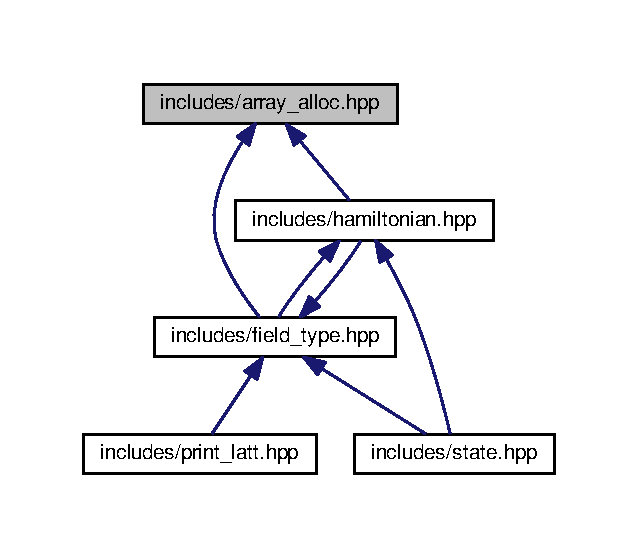
\includegraphics[width=306pt]{d9/d10/array__alloc_8hpp__dep__incl}
\end{center}
\end{figure}
\subsection*{Functions}
\begin{DoxyCompactItemize}
\item 
{\footnotesize template$<$class T $>$ }\\T $\ast$ \hyperlink{array__alloc_8hpp_acff811ea99d964e00d672cc95026ab15}{alloc\+\_\+1darr} (int size\+\_\+m)
\item 
{\footnotesize template$<$class T $>$ }\\T $\ast$$\ast$ \hyperlink{array__alloc_8hpp_a44be4b8a61e758d0bae645e4ea0d2184}{alloc\+\_\+2darr} (int size\+\_\+m, int size\+\_\+n, bool contig=true)
\item 
{\footnotesize template$<$class T $>$ }\\T $\ast$$\ast$$\ast$ \hyperlink{array__alloc_8hpp_a7ed16b3c98dbd7a82d0a85e3f594a5a4}{alloc\+\_\+3darr} (int size\+\_\+m, int size\+\_\+n, int size\+\_\+p, bool contig=true)
\item 
{\footnotesize template$<$class T $>$ }\\void \hyperlink{array__alloc_8hpp_ac95d588ace0250532e4f45d43fd5c5f0}{dealloc\+\_\+1darr} (T $\ast$arr)
\item 
{\footnotesize template$<$class T $>$ }\\void \hyperlink{array__alloc_8hpp_a9783541a0bfc590254a3592037b975f6}{dealloc\+\_\+2darr} (int size\+\_\+m, T $\ast$$\ast$arr, bool contig=true)
\item 
{\footnotesize template$<$class T $>$ }\\void \hyperlink{array__alloc_8hpp_a9e2e849a5e7dabd09755a9007c5cf274}{dealloc\+\_\+3darr} (int size\+\_\+m, int size\+\_\+n, T $\ast$$\ast$$\ast$arr, bool contig=true)
\item 
{\footnotesize template$<$class T $>$ }\\T $\ast$ \hyperlink{array__alloc_8hpp_a1495afadb0decd0d3dc535f202c9480f}{deep\+\_\+copy\+\_\+1darr} (int size\+\_\+m, T $\ast$arr)
\item 
{\footnotesize template$<$class T $>$ }\\T $\ast$$\ast$ \hyperlink{array__alloc_8hpp_a5d35f25188bbca18ce7abca7b02ba5f9}{deep\+\_\+copy\+\_\+2darr} (int size\+\_\+m, int size\+\_\+n, T $\ast$$\ast$arr, bool contig=true)
\item 
{\footnotesize template$<$class T $>$ }\\T $\ast$$\ast$$\ast$ \hyperlink{array__alloc_8hpp_ad25d717436b799cec453fc2d288a1b91}{deep\+\_\+copy\+\_\+3darr} (int size\+\_\+m, int size\+\_\+n, int size\+\_\+p, T $\ast$$\ast$$\ast$arr, bool contig=true)
\end{DoxyCompactItemize}


\subsection{Function Documentation}
\index{array\+\_\+alloc.\+hpp@{array\+\_\+alloc.\+hpp}!alloc\+\_\+1darr@{alloc\+\_\+1darr}}
\index{alloc\+\_\+1darr@{alloc\+\_\+1darr}!array\+\_\+alloc.\+hpp@{array\+\_\+alloc.\+hpp}}
\subsubsection[{\texorpdfstring{alloc\+\_\+1darr(int size\+\_\+m)}{alloc_1darr(int size_m)}}]{\setlength{\rightskip}{0pt plus 5cm}template$<$class T $>$ T$\ast$ alloc\+\_\+1darr (
\begin{DoxyParamCaption}
\item[{int}]{size\+\_\+m}
\end{DoxyParamCaption}
)}\hypertarget{array__alloc_8hpp_acff811ea99d964e00d672cc95026ab15}{}\label{array__alloc_8hpp_acff811ea99d964e00d672cc95026ab15}
\index{array\+\_\+alloc.\+hpp@{array\+\_\+alloc.\+hpp}!alloc\+\_\+2darr@{alloc\+\_\+2darr}}
\index{alloc\+\_\+2darr@{alloc\+\_\+2darr}!array\+\_\+alloc.\+hpp@{array\+\_\+alloc.\+hpp}}
\subsubsection[{\texorpdfstring{alloc\+\_\+2darr(int size\+\_\+m, int size\+\_\+n, bool contig=true)}{alloc_2darr(int size_m, int size_n, bool contig=true)}}]{\setlength{\rightskip}{0pt plus 5cm}template$<$class T $>$ T$\ast$$\ast$ alloc\+\_\+2darr (
\begin{DoxyParamCaption}
\item[{int}]{size\+\_\+m, }
\item[{int}]{size\+\_\+n, }
\item[{bool}]{contig = {\ttfamily true}}
\end{DoxyParamCaption}
)}\hypertarget{array__alloc_8hpp_a44be4b8a61e758d0bae645e4ea0d2184}{}\label{array__alloc_8hpp_a44be4b8a61e758d0bae645e4ea0d2184}
\index{array\+\_\+alloc.\+hpp@{array\+\_\+alloc.\+hpp}!alloc\+\_\+3darr@{alloc\+\_\+3darr}}
\index{alloc\+\_\+3darr@{alloc\+\_\+3darr}!array\+\_\+alloc.\+hpp@{array\+\_\+alloc.\+hpp}}
\subsubsection[{\texorpdfstring{alloc\+\_\+3darr(int size\+\_\+m, int size\+\_\+n, int size\+\_\+p, bool contig=true)}{alloc_3darr(int size_m, int size_n, int size_p, bool contig=true)}}]{\setlength{\rightskip}{0pt plus 5cm}template$<$class T $>$ T$\ast$$\ast$$\ast$ alloc\+\_\+3darr (
\begin{DoxyParamCaption}
\item[{int}]{size\+\_\+m, }
\item[{int}]{size\+\_\+n, }
\item[{int}]{size\+\_\+p, }
\item[{bool}]{contig = {\ttfamily true}}
\end{DoxyParamCaption}
)}\hypertarget{array__alloc_8hpp_a7ed16b3c98dbd7a82d0a85e3f594a5a4}{}\label{array__alloc_8hpp_a7ed16b3c98dbd7a82d0a85e3f594a5a4}
\index{array\+\_\+alloc.\+hpp@{array\+\_\+alloc.\+hpp}!dealloc\+\_\+1darr@{dealloc\+\_\+1darr}}
\index{dealloc\+\_\+1darr@{dealloc\+\_\+1darr}!array\+\_\+alloc.\+hpp@{array\+\_\+alloc.\+hpp}}
\subsubsection[{\texorpdfstring{dealloc\+\_\+1darr(\+T $\ast$arr)}{dealloc_1darr(T *arr)}}]{\setlength{\rightskip}{0pt plus 5cm}template$<$class T $>$ void dealloc\+\_\+1darr (
\begin{DoxyParamCaption}
\item[{T $\ast$}]{arr}
\end{DoxyParamCaption}
)}\hypertarget{array__alloc_8hpp_ac95d588ace0250532e4f45d43fd5c5f0}{}\label{array__alloc_8hpp_ac95d588ace0250532e4f45d43fd5c5f0}
\index{array\+\_\+alloc.\+hpp@{array\+\_\+alloc.\+hpp}!dealloc\+\_\+2darr@{dealloc\+\_\+2darr}}
\index{dealloc\+\_\+2darr@{dealloc\+\_\+2darr}!array\+\_\+alloc.\+hpp@{array\+\_\+alloc.\+hpp}}
\subsubsection[{\texorpdfstring{dealloc\+\_\+2darr(int size\+\_\+m, T $\ast$$\ast$arr, bool contig=true)}{dealloc_2darr(int size_m, T **arr, bool contig=true)}}]{\setlength{\rightskip}{0pt plus 5cm}template$<$class T $>$ void dealloc\+\_\+2darr (
\begin{DoxyParamCaption}
\item[{int}]{size\+\_\+m, }
\item[{T $\ast$$\ast$}]{arr, }
\item[{bool}]{contig = {\ttfamily true}}
\end{DoxyParamCaption}
)}\hypertarget{array__alloc_8hpp_a9783541a0bfc590254a3592037b975f6}{}\label{array__alloc_8hpp_a9783541a0bfc590254a3592037b975f6}
\index{array\+\_\+alloc.\+hpp@{array\+\_\+alloc.\+hpp}!dealloc\+\_\+3darr@{dealloc\+\_\+3darr}}
\index{dealloc\+\_\+3darr@{dealloc\+\_\+3darr}!array\+\_\+alloc.\+hpp@{array\+\_\+alloc.\+hpp}}
\subsubsection[{\texorpdfstring{dealloc\+\_\+3darr(int size\+\_\+m, int size\+\_\+n, T $\ast$$\ast$$\ast$arr, bool contig=true)}{dealloc_3darr(int size_m, int size_n, T ***arr, bool contig=true)}}]{\setlength{\rightskip}{0pt plus 5cm}template$<$class T $>$ void dealloc\+\_\+3darr (
\begin{DoxyParamCaption}
\item[{int}]{size\+\_\+m, }
\item[{int}]{size\+\_\+n, }
\item[{T $\ast$$\ast$$\ast$}]{arr, }
\item[{bool}]{contig = {\ttfamily true}}
\end{DoxyParamCaption}
)}\hypertarget{array__alloc_8hpp_a9e2e849a5e7dabd09755a9007c5cf274}{}\label{array__alloc_8hpp_a9e2e849a5e7dabd09755a9007c5cf274}
\index{array\+\_\+alloc.\+hpp@{array\+\_\+alloc.\+hpp}!deep\+\_\+copy\+\_\+1darr@{deep\+\_\+copy\+\_\+1darr}}
\index{deep\+\_\+copy\+\_\+1darr@{deep\+\_\+copy\+\_\+1darr}!array\+\_\+alloc.\+hpp@{array\+\_\+alloc.\+hpp}}
\subsubsection[{\texorpdfstring{deep\+\_\+copy\+\_\+1darr(int size\+\_\+m, T $\ast$arr)}{deep_copy_1darr(int size_m, T *arr)}}]{\setlength{\rightskip}{0pt plus 5cm}template$<$class T $>$ T$\ast$ deep\+\_\+copy\+\_\+1darr (
\begin{DoxyParamCaption}
\item[{int}]{size\+\_\+m, }
\item[{T $\ast$}]{arr}
\end{DoxyParamCaption}
)}\hypertarget{array__alloc_8hpp_a1495afadb0decd0d3dc535f202c9480f}{}\label{array__alloc_8hpp_a1495afadb0decd0d3dc535f202c9480f}
\index{array\+\_\+alloc.\+hpp@{array\+\_\+alloc.\+hpp}!deep\+\_\+copy\+\_\+2darr@{deep\+\_\+copy\+\_\+2darr}}
\index{deep\+\_\+copy\+\_\+2darr@{deep\+\_\+copy\+\_\+2darr}!array\+\_\+alloc.\+hpp@{array\+\_\+alloc.\+hpp}}
\subsubsection[{\texorpdfstring{deep\+\_\+copy\+\_\+2darr(int size\+\_\+m, int size\+\_\+n, T $\ast$$\ast$arr, bool contig=true)}{deep_copy_2darr(int size_m, int size_n, T **arr, bool contig=true)}}]{\setlength{\rightskip}{0pt plus 5cm}template$<$class T $>$ T$\ast$$\ast$ deep\+\_\+copy\+\_\+2darr (
\begin{DoxyParamCaption}
\item[{int}]{size\+\_\+m, }
\item[{int}]{size\+\_\+n, }
\item[{T $\ast$$\ast$}]{arr, }
\item[{bool}]{contig = {\ttfamily true}}
\end{DoxyParamCaption}
)}\hypertarget{array__alloc_8hpp_a5d35f25188bbca18ce7abca7b02ba5f9}{}\label{array__alloc_8hpp_a5d35f25188bbca18ce7abca7b02ba5f9}
\index{array\+\_\+alloc.\+hpp@{array\+\_\+alloc.\+hpp}!deep\+\_\+copy\+\_\+3darr@{deep\+\_\+copy\+\_\+3darr}}
\index{deep\+\_\+copy\+\_\+3darr@{deep\+\_\+copy\+\_\+3darr}!array\+\_\+alloc.\+hpp@{array\+\_\+alloc.\+hpp}}
\subsubsection[{\texorpdfstring{deep\+\_\+copy\+\_\+3darr(int size\+\_\+m, int size\+\_\+n, int size\+\_\+p, T $\ast$$\ast$$\ast$arr, bool contig=true)}{deep_copy_3darr(int size_m, int size_n, int size_p, T ***arr, bool contig=true)}}]{\setlength{\rightskip}{0pt plus 5cm}template$<$class T $>$ T$\ast$$\ast$$\ast$ deep\+\_\+copy\+\_\+3darr (
\begin{DoxyParamCaption}
\item[{int}]{size\+\_\+m, }
\item[{int}]{size\+\_\+n, }
\item[{int}]{size\+\_\+p, }
\item[{T $\ast$$\ast$$\ast$}]{arr, }
\item[{bool}]{contig = {\ttfamily true}}
\end{DoxyParamCaption}
)}\hypertarget{array__alloc_8hpp_ad25d717436b799cec453fc2d288a1b91}{}\label{array__alloc_8hpp_ad25d717436b799cec453fc2d288a1b91}

\hypertarget{field__type_8hpp}{}\section{includes/field\+\_\+type.hpp File Reference}
\label{field__type_8hpp}\index{includes/field\+\_\+type.\+hpp@{includes/field\+\_\+type.\+hpp}}
{\ttfamily \#include \char`\"{}hamiltonian.\+hpp\char`\"{}}\\*
{\ttfamily \#include \char`\"{}array\+\_\+alloc.\+hpp\char`\"{}}\\*
{\ttfamily \#include $<$vector$>$}\\*
{\ttfamily \#include $<$string$>$}\\*
Include dependency graph for field\+\_\+type.\+hpp\+:\nopagebreak
\begin{figure}[H]
\begin{center}
\leavevmode
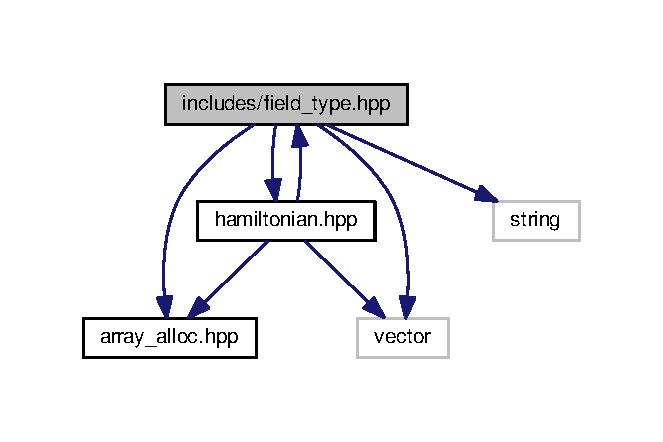
\includegraphics[width=318pt]{d0/dfc/field__type_8hpp__incl}
\end{center}
\end{figure}
This graph shows which files directly or indirectly include this file\+:\nopagebreak
\begin{figure}[H]
\begin{center}
\leavevmode
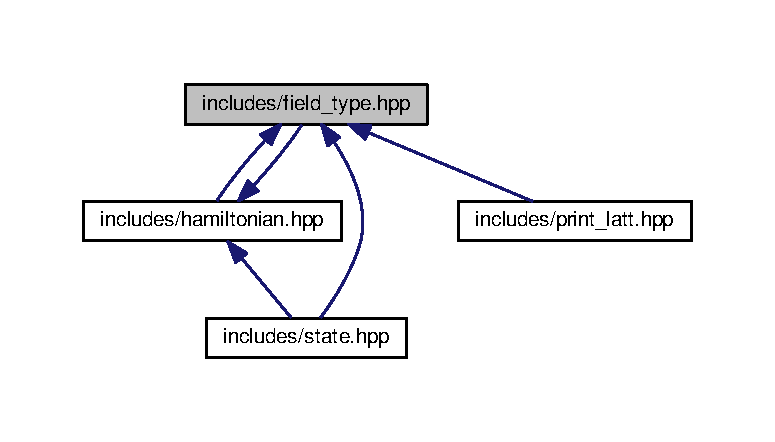
\includegraphics[width=350pt]{db/df2/field__type_8hpp__dep__incl}
\end{center}
\end{figure}
\subsection*{Classes}
\begin{DoxyCompactItemize}
\item 
class \hyperlink{classfield__type}{field\+\_\+type}
\item 
class \hyperlink{classfield__cluster__h}{field\+\_\+cluster\+\_\+h}
\item 
class \hyperlink{classfield__2d}{field\+\_\+2d}
\item 
class \hyperlink{classfield__2d__h}{field\+\_\+2d\+\_\+h}
\item 
class \hyperlink{classfield__2d__i}{field\+\_\+2d\+\_\+i}
\item 
class \hyperlink{classfield__3d}{field\+\_\+3d}
\item 
class \hyperlink{classfield__3d__h}{field\+\_\+3d\+\_\+h}
\item 
class \hyperlink{classfield__3d__i}{field\+\_\+3d\+\_\+i}
\end{DoxyCompactItemize}
\subsection*{Functions}
\begin{DoxyCompactItemize}
\item 
void \hyperlink{field__type_8hpp_a3046d14208aa841cfab95127dcd36748}{rand\+\_\+spin\+\_\+h} (double \&x, double \&y, double \&z)
\end{DoxyCompactItemize}


\subsection{Function Documentation}
\index{field\+\_\+type.\+hpp@{field\+\_\+type.\+hpp}!rand\+\_\+spin\+\_\+h@{rand\+\_\+spin\+\_\+h}}
\index{rand\+\_\+spin\+\_\+h@{rand\+\_\+spin\+\_\+h}!field\+\_\+type.\+hpp@{field\+\_\+type.\+hpp}}
\subsubsection[{\texorpdfstring{rand\+\_\+spin\+\_\+h(double \&x, double \&y, double \&z)}{rand_spin_h(double &x, double &y, double &z)}}]{\setlength{\rightskip}{0pt plus 5cm}void rand\+\_\+spin\+\_\+h (
\begin{DoxyParamCaption}
\item[{double \&}]{x, }
\item[{double \&}]{y, }
\item[{double \&}]{z}
\end{DoxyParamCaption}
)}\hypertarget{field__type_8hpp_a3046d14208aa841cfab95127dcd36748}{}\label{field__type_8hpp_a3046d14208aa841cfab95127dcd36748}

\hypertarget{functions_8hpp}{}\section{includes/functions.hpp File Reference}
\label{functions_8hpp}\index{includes/functions.\+hpp@{includes/functions.\+hpp}}
{\ttfamily \#include $<$vector$>$}\\*
{\ttfamily \#include $<$fstream$>$}\\*
{\ttfamily \#include $<$cstring$>$}\\*
Include dependency graph for functions.\+hpp\+:
\nopagebreak
\begin{figure}[H]
\begin{center}
\leavevmode
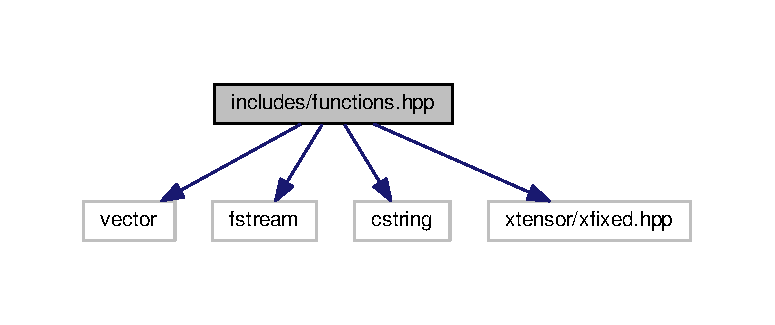
\includegraphics[width=256pt]{d9/dbc/functions_8hpp__incl}
\end{center}
\end{figure}
\subsection*{Functions}
\begin{DoxyCompactItemize}
\item 
double \hyperlink{functions_8hpp_ac8b8c6cfe216441c239a5141d8b91572}{mean} (std\+::vector$<$ double $>$ \&oY)
\item 
double \hyperlink{functions_8hpp_aa1d01024ee5111011608f75db463fac5}{std\+\_\+dev} (std\+::vector$<$ double $>$ \&x)
\item 
double \hyperlink{functions_8hpp_a1ece0bbde6352f3b8e9d568770594a4c}{norm} (std\+::vector$<$ double $>$ vals)
\item 
double \hyperlink{functions_8hpp_afc9dbcc07461e220f40e6e07d21c572b}{sum} (std\+::vector$<$ double $>$ \&oY)
\item 
int \hyperlink{functions_8hpp_a463977d9d5ba775174a78fbf9d825a25}{sum} (std\+::vector$<$ int $>$ \&oY)
\item 
void \hyperlink{functions_8hpp_a34f099021e0d8fa3bf9258fddb37cf35}{Ato\+Ln} (double amean, double asd, double \&lmean, double \&lsd)
\item 
int \hyperlink{functions_8hpp_a69c18c9507ef22a89f1f437bcc75baaf}{mod} (int a, int b)
\item 
double \hyperlink{functions_8hpp_af6a509563a962606266a025475e31470}{solid\+\_\+angle} (const std\+::vector$<$ double $>$ \&s1, const std\+::vector$<$ double $>$ \&s2, const std\+::vector$<$ double $>$ \&s3, std\+::vector$<$ double $>$ \&buff)
\end{DoxyCompactItemize}


\subsection{Function Documentation}
\index{functions.\+hpp@{functions.\+hpp}!Ato\+Ln@{Ato\+Ln}}
\index{Ato\+Ln@{Ato\+Ln}!functions.\+hpp@{functions.\+hpp}}
\subsubsection[{\texorpdfstring{Ato\+Ln(double amean, double asd, double \&lmean, double \&lsd)}{AtoLn(double amean, double asd, double &lmean, double &lsd)}}]{\setlength{\rightskip}{0pt plus 5cm}void Ato\+Ln (
\begin{DoxyParamCaption}
\item[{double}]{amean, }
\item[{double}]{asd, }
\item[{double \&}]{lmean, }
\item[{double \&}]{lsd}
\end{DoxyParamCaption}
)}\hypertarget{functions_8hpp_a34f099021e0d8fa3bf9258fddb37cf35}{}\label{functions_8hpp_a34f099021e0d8fa3bf9258fddb37cf35}
\index{functions.\+hpp@{functions.\+hpp}!mean@{mean}}
\index{mean@{mean}!functions.\+hpp@{functions.\+hpp}}
\subsubsection[{\texorpdfstring{mean(std\+::vector$<$ double $>$ \&o\+Y)}{mean(std::vector< double > &oY)}}]{\setlength{\rightskip}{0pt plus 5cm}double mean (
\begin{DoxyParamCaption}
\item[{std\+::vector$<$ double $>$ \&}]{oY}
\end{DoxyParamCaption}
)}\hypertarget{functions_8hpp_ac8b8c6cfe216441c239a5141d8b91572}{}\label{functions_8hpp_ac8b8c6cfe216441c239a5141d8b91572}
\index{functions.\+hpp@{functions.\+hpp}!mod@{mod}}
\index{mod@{mod}!functions.\+hpp@{functions.\+hpp}}
\subsubsection[{\texorpdfstring{mod(int a, int b)}{mod(int a, int b)}}]{\setlength{\rightskip}{0pt plus 5cm}int mod (
\begin{DoxyParamCaption}
\item[{int}]{a, }
\item[{int}]{b}
\end{DoxyParamCaption}
)}\hypertarget{functions_8hpp_a69c18c9507ef22a89f1f437bcc75baaf}{}\label{functions_8hpp_a69c18c9507ef22a89f1f437bcc75baaf}
\index{functions.\+hpp@{functions.\+hpp}!norm@{norm}}
\index{norm@{norm}!functions.\+hpp@{functions.\+hpp}}
\subsubsection[{\texorpdfstring{norm(std\+::vector$<$ double $>$ vals)}{norm(std::vector< double > vals)}}]{\setlength{\rightskip}{0pt plus 5cm}double norm (
\begin{DoxyParamCaption}
\item[{std\+::vector$<$ double $>$}]{vals}
\end{DoxyParamCaption}
)}\hypertarget{functions_8hpp_a1ece0bbde6352f3b8e9d568770594a4c}{}\label{functions_8hpp_a1ece0bbde6352f3b8e9d568770594a4c}
\index{functions.\+hpp@{functions.\+hpp}!solid\+\_\+angle@{solid\+\_\+angle}}
\index{solid\+\_\+angle@{solid\+\_\+angle}!functions.\+hpp@{functions.\+hpp}}
\subsubsection[{\texorpdfstring{solid\+\_\+angle(const std\+::vector$<$ double $>$ \&s1, const std\+::vector$<$ double $>$ \&s2, const std\+::vector$<$ double $>$ \&s3, std\+::vector$<$ double $>$ \&buff)}{solid_angle(const std::vector< double > &s1, const std::vector< double > &s2, const std::vector< double > &s3, std::vector< double > &buff)}}]{\setlength{\rightskip}{0pt plus 5cm}double solid\+\_\+angle (
\begin{DoxyParamCaption}
\item[{const std\+::vector$<$ double $>$ \&}]{s1, }
\item[{const std\+::vector$<$ double $>$ \&}]{s2, }
\item[{const std\+::vector$<$ double $>$ \&}]{s3, }
\item[{std\+::vector$<$ double $>$ \&}]{buff}
\end{DoxyParamCaption}
)}\hypertarget{functions_8hpp_af6a509563a962606266a025475e31470}{}\label{functions_8hpp_af6a509563a962606266a025475e31470}
\index{functions.\+hpp@{functions.\+hpp}!std\+\_\+dev@{std\+\_\+dev}}
\index{std\+\_\+dev@{std\+\_\+dev}!functions.\+hpp@{functions.\+hpp}}
\subsubsection[{\texorpdfstring{std\+\_\+dev(std\+::vector$<$ double $>$ \&x)}{std_dev(std::vector< double > &x)}}]{\setlength{\rightskip}{0pt plus 5cm}double std\+\_\+dev (
\begin{DoxyParamCaption}
\item[{std\+::vector$<$ double $>$ \&}]{x}
\end{DoxyParamCaption}
)}\hypertarget{functions_8hpp_aa1d01024ee5111011608f75db463fac5}{}\label{functions_8hpp_aa1d01024ee5111011608f75db463fac5}
\index{functions.\+hpp@{functions.\+hpp}!sum@{sum}}
\index{sum@{sum}!functions.\+hpp@{functions.\+hpp}}
\subsubsection[{\texorpdfstring{sum(std\+::vector$<$ double $>$ \&o\+Y)}{sum(std::vector< double > &oY)}}]{\setlength{\rightskip}{0pt plus 5cm}double sum (
\begin{DoxyParamCaption}
\item[{std\+::vector$<$ double $>$ \&}]{oY}
\end{DoxyParamCaption}
)}\hypertarget{functions_8hpp_afc9dbcc07461e220f40e6e07d21c572b}{}\label{functions_8hpp_afc9dbcc07461e220f40e6e07d21c572b}
\index{functions.\+hpp@{functions.\+hpp}!sum@{sum}}
\index{sum@{sum}!functions.\+hpp@{functions.\+hpp}}
\subsubsection[{\texorpdfstring{sum(std\+::vector$<$ int $>$ \&o\+Y)}{sum(std::vector< int > &oY)}}]{\setlength{\rightskip}{0pt plus 5cm}int sum (
\begin{DoxyParamCaption}
\item[{std\+::vector$<$ int $>$ \&}]{oY}
\end{DoxyParamCaption}
)}\hypertarget{functions_8hpp_a463977d9d5ba775174a78fbf9d825a25}{}\label{functions_8hpp_a463977d9d5ba775174a78fbf9d825a25}

\hypertarget{output_8hpp}{}\section{includes/output.hpp File Reference}
\label{output_8hpp}\index{includes/output.\+hpp@{includes/output.\+hpp}}
{\ttfamily \#include \char`\"{}param\+\_\+read.\+hpp\char`\"{}}\\*
{\ttfamily \#include $<$fstream$>$}\\*
{\ttfamily \#include $<$cstring$>$}\\*
Include dependency graph for output.\+hpp\+:\nopagebreak
\begin{figure}[H]
\begin{center}
\leavevmode
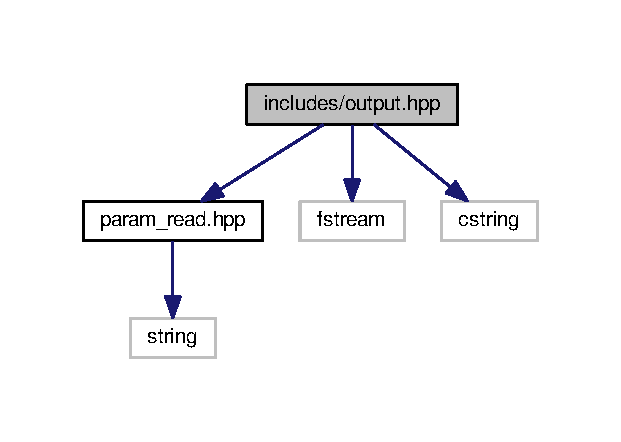
\includegraphics[width=298pt]{d5/d35/output_8hpp__incl}
\end{center}
\end{figure}
\subsection*{Functions}
\begin{DoxyCompactItemize}
\item 
void \hyperlink{output_8hpp_a1d0046dcf4f96b0e81ee2c32fbf50170}{check\+\_\+h5\+\_\+file} (\hyperlink{structstateOptions}{state\+Options} \&st\+Opt, \hyperlink{structsimOptions}{sim\+Options} \&sim\+Opt, const int num\+\_\+\+Ts, const int num\+\_\+\+Hs, const float $\ast$Ts, const float $\ast$Hs, const int v1\+\_\+size, bool $\ast$$\ast$checkp, bool \&file\+\_\+exists)
\item 
void \hyperlink{output_8hpp_a917aef04c3f8e6f3efab883505b69d63}{create\+\_\+h5\+\_\+file} (\hyperlink{structstateOptions}{state\+Options} \&st\+Opt, \hyperlink{structsimOptions}{sim\+Options} \&sim\+Opt, const int num\+\_\+\+Ts, const int num\+\_\+\+Hs, const float $\ast$Ts, const float $\ast$Hs, const int v1\+\_\+size)
\item 
void \hyperlink{output_8hpp_a5152c310605eb4363607d530c5d149bc}{print\+\_\+\+T\+D\+\_\+h5} (const float $\ast$magx, const float $\ast$magy, const float $\ast$magz, const float $\ast$mag, const float $\ast$ener, const float $\ast$smagx, const float $\ast$smagy, const float $\ast$smagz, const float $\ast$smag, float $\ast$$\ast$tcs, \hyperlink{structstateOptions}{state\+Options} st\+Opt, \hyperlink{structsimOptions}{sim\+Options} sim\+Opt, const int var1, const int var2, const int v2max, const int latt\+\_\+num)
\end{DoxyCompactItemize}


\subsection{Function Documentation}
\index{output.\+hpp@{output.\+hpp}!check\+\_\+h5\+\_\+file@{check\+\_\+h5\+\_\+file}}
\index{check\+\_\+h5\+\_\+file@{check\+\_\+h5\+\_\+file}!output.\+hpp@{output.\+hpp}}
\subsubsection[{\texorpdfstring{check\+\_\+h5\+\_\+file(state\+Options \&st\+Opt, sim\+Options \&sim\+Opt, const int num\+\_\+\+Ts, const int num\+\_\+\+Hs, const float $\ast$\+Ts, const float $\ast$\+Hs, const int v1\+\_\+size, bool $\ast$$\ast$checkp, bool \&file\+\_\+exists)}{check_h5_file(stateOptions &stOpt, simOptions &simOpt, const int num_Ts, const int num_Hs, const float *Ts, const float *Hs, const int v1_size, bool **checkp, bool &file_exists)}}]{\setlength{\rightskip}{0pt plus 5cm}void check\+\_\+h5\+\_\+file (
\begin{DoxyParamCaption}
\item[{{\bf state\+Options} \&}]{st\+Opt, }
\item[{{\bf sim\+Options} \&}]{sim\+Opt, }
\item[{const int}]{num\+\_\+\+Ts, }
\item[{const int}]{num\+\_\+\+Hs, }
\item[{const float $\ast$}]{Ts, }
\item[{const float $\ast$}]{Hs, }
\item[{const int}]{v1\+\_\+size, }
\item[{bool $\ast$$\ast$}]{checkp, }
\item[{bool \&}]{file\+\_\+exists}
\end{DoxyParamCaption}
)}\hypertarget{output_8hpp_a1d0046dcf4f96b0e81ee2c32fbf50170}{}\label{output_8hpp_a1d0046dcf4f96b0e81ee2c32fbf50170}
\index{output.\+hpp@{output.\+hpp}!create\+\_\+h5\+\_\+file@{create\+\_\+h5\+\_\+file}}
\index{create\+\_\+h5\+\_\+file@{create\+\_\+h5\+\_\+file}!output.\+hpp@{output.\+hpp}}
\subsubsection[{\texorpdfstring{create\+\_\+h5\+\_\+file(state\+Options \&st\+Opt, sim\+Options \&sim\+Opt, const int num\+\_\+\+Ts, const int num\+\_\+\+Hs, const float $\ast$\+Ts, const float $\ast$\+Hs, const int v1\+\_\+size)}{create_h5_file(stateOptions &stOpt, simOptions &simOpt, const int num_Ts, const int num_Hs, const float *Ts, const float *Hs, const int v1_size)}}]{\setlength{\rightskip}{0pt plus 5cm}void create\+\_\+h5\+\_\+file (
\begin{DoxyParamCaption}
\item[{{\bf state\+Options} \&}]{st\+Opt, }
\item[{{\bf sim\+Options} \&}]{sim\+Opt, }
\item[{const int}]{num\+\_\+\+Ts, }
\item[{const int}]{num\+\_\+\+Hs, }
\item[{const float $\ast$}]{Ts, }
\item[{const float $\ast$}]{Hs, }
\item[{const int}]{v1\+\_\+size}
\end{DoxyParamCaption}
)}\hypertarget{output_8hpp_a917aef04c3f8e6f3efab883505b69d63}{}\label{output_8hpp_a917aef04c3f8e6f3efab883505b69d63}
\index{output.\+hpp@{output.\+hpp}!print\+\_\+\+T\+D\+\_\+h5@{print\+\_\+\+T\+D\+\_\+h5}}
\index{print\+\_\+\+T\+D\+\_\+h5@{print\+\_\+\+T\+D\+\_\+h5}!output.\+hpp@{output.\+hpp}}
\subsubsection[{\texorpdfstring{print\+\_\+\+T\+D\+\_\+h5(const float $\ast$magx, const float $\ast$magy, const float $\ast$magz, const float $\ast$mag, const float $\ast$ener, const float $\ast$smagx, const float $\ast$smagy, const float $\ast$smagz, const float $\ast$smag, float $\ast$$\ast$tcs, state\+Options st\+Opt, sim\+Options sim\+Opt, const int var1, const int var2, const int v2max, const int latt\+\_\+num)}{print_TD_h5(const float *magx, const float *magy, const float *magz, const float *mag, const float *ener, const float *smagx, const float *smagy, const float *smagz, const float *smag, float **tcs, stateOptions stOpt, simOptions simOpt, const int var1, const int var2, const int v2max, const int latt_num)}}]{\setlength{\rightskip}{0pt plus 5cm}void print\+\_\+\+T\+D\+\_\+h5 (
\begin{DoxyParamCaption}
\item[{const float $\ast$}]{magx, }
\item[{const float $\ast$}]{magy, }
\item[{const float $\ast$}]{magz, }
\item[{const float $\ast$}]{mag, }
\item[{const float $\ast$}]{ener, }
\item[{const float $\ast$}]{smagx, }
\item[{const float $\ast$}]{smagy, }
\item[{const float $\ast$}]{smagz, }
\item[{const float $\ast$}]{smag, }
\item[{float $\ast$$\ast$}]{tcs, }
\item[{{\bf state\+Options}}]{st\+Opt, }
\item[{{\bf sim\+Options}}]{sim\+Opt, }
\item[{const int}]{var1, }
\item[{const int}]{var2, }
\item[{const int}]{v2max, }
\item[{const int}]{latt\+\_\+num}
\end{DoxyParamCaption}
)}\hypertarget{output_8hpp_a5152c310605eb4363607d530c5d149bc}{}\label{output_8hpp_a5152c310605eb4363607d530c5d149bc}

\hypertarget{param__read_8hpp}{}\section{includes/param\+\_\+read.hpp File Reference}
\label{param__read_8hpp}\index{includes/param\+\_\+read.\+hpp@{includes/param\+\_\+read.\+hpp}}
{\ttfamily \#include $<$string$>$}\\*
Include dependency graph for param\+\_\+read.\+hpp\+:
\nopagebreak
\begin{figure}[H]
\begin{center}
\leavevmode
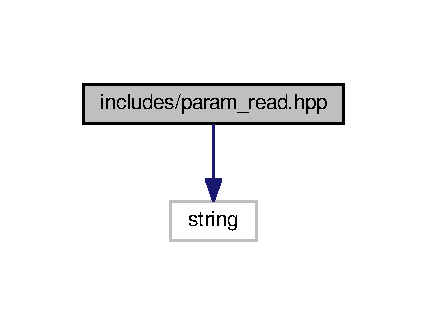
\includegraphics[width=205pt]{d8/de7/param__read_8hpp__incl}
\end{center}
\end{figure}
\subsection*{Functions}
\begin{DoxyCompactItemize}
\item 
{\footnotesize template$<$class T $>$ }\\T \hyperlink{param__read_8hpp_acfcd9e62d947339a9fd8b3339d014925}{read\+\_\+var} (std\+::string v\+\_\+name, std\+::string f\+\_\+name)
\item 
void \hyperlink{param__read_8hpp_a3c76a03037ab020686fdd13c0d94efcc}{read\+\_\+all\+\_\+vars} (std\+::string f\+\_\+name, double \&size, double \&J, double \&k, bool \&periodic, char \&shape, char \&hamil, int \&Samp\+\_\+steps, int \&N\+\_\+samp, int \&Eq\+\_\+steps, int \&N\+\_\+latts, double \&beta, bool \&distrib, double \&amean, double \&asd, std\+::string \&temp\+\_\+name, std\+::string \&field\+\_\+name, int \&protocol, double \&K, bool \&print\+\_\+latt)
\item 
void \hyperlink{param__read_8hpp_a247c1320a8ff367a58a7bc6897de3ab6}{load\+\_\+\+Hs\+\_\+\+Ts} (std\+::string Tname, float $\ast$\&Ts, int \&Tnum, std\+::string Hname, float $\ast$\&Hs, int \&Hnum)
\end{DoxyCompactItemize}


\subsection{Function Documentation}
\index{param\+\_\+read.\+hpp@{param\+\_\+read.\+hpp}!load\+\_\+\+Hs\+\_\+\+Ts@{load\+\_\+\+Hs\+\_\+\+Ts}}
\index{load\+\_\+\+Hs\+\_\+\+Ts@{load\+\_\+\+Hs\+\_\+\+Ts}!param\+\_\+read.\+hpp@{param\+\_\+read.\+hpp}}
\subsubsection[{\texorpdfstring{load\+\_\+\+Hs\+\_\+\+Ts(std\+::string Tname, float $\ast$\&\+Ts, int \&\+Tnum, std\+::string Hname, float $\ast$\&\+Hs, int \&\+Hnum)}{load_Hs_Ts(std::string Tname, float *&Ts, int &Tnum, std::string Hname, float *&Hs, int &Hnum)}}]{\setlength{\rightskip}{0pt plus 5cm}void load\+\_\+\+Hs\+\_\+\+Ts (
\begin{DoxyParamCaption}
\item[{std\+::string}]{Tname, }
\item[{float $\ast$\&}]{Ts, }
\item[{int \&}]{Tnum, }
\item[{std\+::string}]{Hname, }
\item[{float $\ast$\&}]{Hs, }
\item[{int \&}]{Hnum}
\end{DoxyParamCaption}
)}\hypertarget{param__read_8hpp_a247c1320a8ff367a58a7bc6897de3ab6}{}\label{param__read_8hpp_a247c1320a8ff367a58a7bc6897de3ab6}
\index{param\+\_\+read.\+hpp@{param\+\_\+read.\+hpp}!read\+\_\+all\+\_\+vars@{read\+\_\+all\+\_\+vars}}
\index{read\+\_\+all\+\_\+vars@{read\+\_\+all\+\_\+vars}!param\+\_\+read.\+hpp@{param\+\_\+read.\+hpp}}
\subsubsection[{\texorpdfstring{read\+\_\+all\+\_\+vars(std\+::string f\+\_\+name, double \&size, double \&\+J, double \&k, bool \&periodic, char \&shape, char \&hamil, int \&\+Samp\+\_\+steps, int \&\+N\+\_\+samp, int \&\+Eq\+\_\+steps, int \&\+N\+\_\+latts, double \&beta, bool \&distrib, double \&amean, double \&asd, std\+::string \&temp\+\_\+name, std\+::string \&field\+\_\+name, int \&protocol, double \&\+K, bool \&print\+\_\+latt)}{read_all_vars(std::string f_name, double &size, double &J, double &k, bool &periodic, char &shape, char &hamil, int &Samp_steps, int &N_samp, int &Eq_steps, int &N_latts, double &beta, bool &distrib, double &amean, double &asd, std::string &temp_name, std::string &field_name, int &protocol, double &K, bool &print_latt)}}]{\setlength{\rightskip}{0pt plus 5cm}void read\+\_\+all\+\_\+vars (
\begin{DoxyParamCaption}
\item[{std\+::string}]{f\+\_\+name, }
\item[{double \&}]{size, }
\item[{double \&}]{J, }
\item[{double \&}]{k, }
\item[{bool \&}]{periodic, }
\item[{char \&}]{shape, }
\item[{char \&}]{hamil, }
\item[{int \&}]{Samp\+\_\+steps, }
\item[{int \&}]{N\+\_\+samp, }
\item[{int \&}]{Eq\+\_\+steps, }
\item[{int \&}]{N\+\_\+latts, }
\item[{double \&}]{beta, }
\item[{bool \&}]{distrib, }
\item[{double \&}]{amean, }
\item[{double \&}]{asd, }
\item[{std\+::string \&}]{temp\+\_\+name, }
\item[{std\+::string \&}]{field\+\_\+name, }
\item[{int \&}]{protocol, }
\item[{double \&}]{K, }
\item[{bool \&}]{print\+\_\+latt}
\end{DoxyParamCaption}
)}\hypertarget{param__read_8hpp_a3c76a03037ab020686fdd13c0d94efcc}{}\label{param__read_8hpp_a3c76a03037ab020686fdd13c0d94efcc}
\index{param\+\_\+read.\+hpp@{param\+\_\+read.\+hpp}!read\+\_\+var@{read\+\_\+var}}
\index{read\+\_\+var@{read\+\_\+var}!param\+\_\+read.\+hpp@{param\+\_\+read.\+hpp}}
\subsubsection[{\texorpdfstring{read\+\_\+var(std\+::string v\+\_\+name, std\+::string f\+\_\+name)}{read_var(std::string v_name, std::string f_name)}}]{\setlength{\rightskip}{0pt plus 5cm}template$<$class T $>$ T read\+\_\+var (
\begin{DoxyParamCaption}
\item[{std\+::string}]{v\+\_\+name, }
\item[{std\+::string}]{f\+\_\+name}
\end{DoxyParamCaption}
)}\hypertarget{param__read_8hpp_acfcd9e62d947339a9fd8b3339d014925}{}\label{param__read_8hpp_acfcd9e62d947339a9fd8b3339d014925}

\hypertarget{print__latt_8hpp}{}\section{includes/print\+\_\+latt.hpp File Reference}
\label{print__latt_8hpp}\index{includes/print\+\_\+latt.\+hpp@{includes/print\+\_\+latt.\+hpp}}
{\ttfamily \#include \char`\"{}field\+\_\+type.\+hpp\char`\"{}}\\*
{\ttfamily \#include $<$cstring$>$}\\*
Include dependency graph for print\+\_\+latt.\+hpp\+:
\nopagebreak
\begin{figure}[H]
\begin{center}
\leavevmode
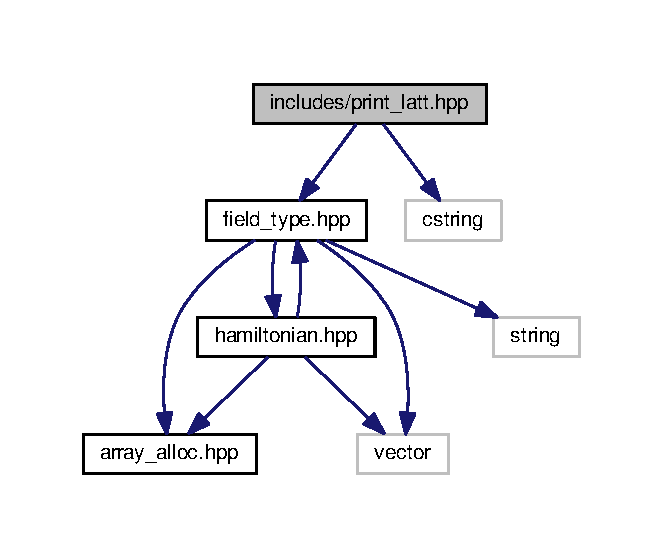
\includegraphics[width=318pt]{d0/dbe/print__latt_8hpp__incl}
\end{center}
\end{figure}
\subsection*{Functions}
\begin{DoxyCompactItemize}
\item 
\hyperlink{classfield__type}{field\+\_\+type} $\ast$ \hyperlink{print__latt_8hpp_a3c777327c17ad81f416b0d5b217226a9}{set\+\_\+sum\+\_\+latt} (double size, bool periodic, char shape, char hamil)
\item 
std\+::string \hyperlink{print__latt_8hpp_a6564bc63113f285facf89e597f876df6}{av\+\_\+latt\+\_\+name} (const int protocol, const int var1, const int var2)
\item 
std\+::string \hyperlink{print__latt_8hpp_aeade27011bb7d5b38e3945af4fa7f4bb}{sing\+\_\+latt\+\_\+name} (const int protocol, const int var1, const int var2)
\end{DoxyCompactItemize}


\subsection{Function Documentation}
\index{print\+\_\+latt.\+hpp@{print\+\_\+latt.\+hpp}!av\+\_\+latt\+\_\+name@{av\+\_\+latt\+\_\+name}}
\index{av\+\_\+latt\+\_\+name@{av\+\_\+latt\+\_\+name}!print\+\_\+latt.\+hpp@{print\+\_\+latt.\+hpp}}
\subsubsection[{\texorpdfstring{av\+\_\+latt\+\_\+name(const int protocol, const int var1, const int var2)}{av_latt_name(const int protocol, const int var1, const int var2)}}]{\setlength{\rightskip}{0pt plus 5cm}std\+::string av\+\_\+latt\+\_\+name (
\begin{DoxyParamCaption}
\item[{const int}]{protocol, }
\item[{const int}]{var1, }
\item[{const int}]{var2}
\end{DoxyParamCaption}
)}\hypertarget{print__latt_8hpp_a6564bc63113f285facf89e597f876df6}{}\label{print__latt_8hpp_a6564bc63113f285facf89e597f876df6}
\index{print\+\_\+latt.\+hpp@{print\+\_\+latt.\+hpp}!set\+\_\+sum\+\_\+latt@{set\+\_\+sum\+\_\+latt}}
\index{set\+\_\+sum\+\_\+latt@{set\+\_\+sum\+\_\+latt}!print\+\_\+latt.\+hpp@{print\+\_\+latt.\+hpp}}
\subsubsection[{\texorpdfstring{set\+\_\+sum\+\_\+latt(double size, bool periodic, char shape, char hamil)}{set_sum_latt(double size, bool periodic, char shape, char hamil)}}]{\setlength{\rightskip}{0pt plus 5cm}{\bf field\+\_\+type}$\ast$ set\+\_\+sum\+\_\+latt (
\begin{DoxyParamCaption}
\item[{double}]{size, }
\item[{bool}]{periodic, }
\item[{char}]{shape, }
\item[{char}]{hamil}
\end{DoxyParamCaption}
)}\hypertarget{print__latt_8hpp_a3c777327c17ad81f416b0d5b217226a9}{}\label{print__latt_8hpp_a3c777327c17ad81f416b0d5b217226a9}
\index{print\+\_\+latt.\+hpp@{print\+\_\+latt.\+hpp}!sing\+\_\+latt\+\_\+name@{sing\+\_\+latt\+\_\+name}}
\index{sing\+\_\+latt\+\_\+name@{sing\+\_\+latt\+\_\+name}!print\+\_\+latt.\+hpp@{print\+\_\+latt.\+hpp}}
\subsubsection[{\texorpdfstring{sing\+\_\+latt\+\_\+name(const int protocol, const int var1, const int var2)}{sing_latt_name(const int protocol, const int var1, const int var2)}}]{\setlength{\rightskip}{0pt plus 5cm}std\+::string sing\+\_\+latt\+\_\+name (
\begin{DoxyParamCaption}
\item[{const int}]{protocol, }
\item[{const int}]{var1, }
\item[{const int}]{var2}
\end{DoxyParamCaption}
)}\hypertarget{print__latt_8hpp_aeade27011bb7d5b38e3945af4fa7f4bb}{}\label{print__latt_8hpp_aeade27011bb7d5b38e3945af4fa7f4bb}

\hypertarget{protocol_8hpp}{}\section{includes/protocol.hpp File Reference}
\label{protocol_8hpp}\index{includes/protocol.\+hpp@{includes/protocol.\+hpp}}
{\ttfamily \#include $<$iostream$>$}\\*
Include dependency graph for protocol.\+hpp\+:\nopagebreak
\begin{figure}[H]
\begin{center}
\leavevmode
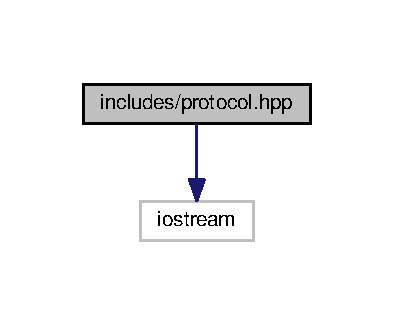
\includegraphics[width=189pt]{d3/d06/protocol_8hpp__incl}
\end{center}
\end{figure}
\subsection*{Functions}
\begin{DoxyCompactItemize}
\item 
void \hyperlink{protocol_8hpp_ac6e6be44297d6f6aadc2aafe1a02d6e8}{set\+\_\+protocol} (const int proto\+\_\+code, float $\ast$\&var1\+\_\+list, float $\ast$\&var2\+\_\+list, int \&var1\+\_\+size, int \&var2\+\_\+size, int \&var1\+\_\+begin, int \&var2\+\_\+begin, int \&var1\+\_\+end, int \&var2\+\_\+end, int \&var1\+\_\+final, float $\ast$Hs, float $\ast$Ts, const int H\+\_\+size, const int T\+\_\+size)
\item 
void \hyperlink{protocol_8hpp_a00d9c9379a1162c02e1d56c160dbc984}{incr\+\_\+v1} (const int proto\+\_\+code, int \&var1\+\_\+curr)
\item 
void \hyperlink{protocol_8hpp_a22e55bf0ca86d488ca20ab6bff6ab6fe}{incr\+\_\+v2} (const int proto\+\_\+code, int \&var2\+\_\+curr)
\item 
bool \hyperlink{protocol_8hpp_a34676923926186d6af84544ea03bffdd}{check\+\_\+rank\+\_\+run} (const int proto\+\_\+code, const int i, const int comm\+\_\+size, const int rank, const int var1\+\_\+size)
\end{DoxyCompactItemize}


\subsection{Function Documentation}
\index{protocol.\+hpp@{protocol.\+hpp}!check\+\_\+rank\+\_\+run@{check\+\_\+rank\+\_\+run}}
\index{check\+\_\+rank\+\_\+run@{check\+\_\+rank\+\_\+run}!protocol.\+hpp@{protocol.\+hpp}}
\subsubsection[{\texorpdfstring{check\+\_\+rank\+\_\+run(const int proto\+\_\+code, const int i, const int comm\+\_\+size, const int rank, const int var1\+\_\+size)}{check_rank_run(const int proto_code, const int i, const int comm_size, const int rank, const int var1_size)}}]{\setlength{\rightskip}{0pt plus 5cm}bool check\+\_\+rank\+\_\+run (
\begin{DoxyParamCaption}
\item[{const int}]{proto\+\_\+code, }
\item[{const int}]{i, }
\item[{const int}]{comm\+\_\+size, }
\item[{const int}]{rank, }
\item[{const int}]{var1\+\_\+size}
\end{DoxyParamCaption}
)}\hypertarget{protocol_8hpp_a34676923926186d6af84544ea03bffdd}{}\label{protocol_8hpp_a34676923926186d6af84544ea03bffdd}
\index{protocol.\+hpp@{protocol.\+hpp}!incr\+\_\+v1@{incr\+\_\+v1}}
\index{incr\+\_\+v1@{incr\+\_\+v1}!protocol.\+hpp@{protocol.\+hpp}}
\subsubsection[{\texorpdfstring{incr\+\_\+v1(const int proto\+\_\+code, int \&var1\+\_\+curr)}{incr_v1(const int proto_code, int &var1_curr)}}]{\setlength{\rightskip}{0pt plus 5cm}void incr\+\_\+v1 (
\begin{DoxyParamCaption}
\item[{const int}]{proto\+\_\+code, }
\item[{int \&}]{var1\+\_\+curr}
\end{DoxyParamCaption}
)}\hypertarget{protocol_8hpp_a00d9c9379a1162c02e1d56c160dbc984}{}\label{protocol_8hpp_a00d9c9379a1162c02e1d56c160dbc984}
\index{protocol.\+hpp@{protocol.\+hpp}!incr\+\_\+v2@{incr\+\_\+v2}}
\index{incr\+\_\+v2@{incr\+\_\+v2}!protocol.\+hpp@{protocol.\+hpp}}
\subsubsection[{\texorpdfstring{incr\+\_\+v2(const int proto\+\_\+code, int \&var2\+\_\+curr)}{incr_v2(const int proto_code, int &var2_curr)}}]{\setlength{\rightskip}{0pt plus 5cm}void incr\+\_\+v2 (
\begin{DoxyParamCaption}
\item[{const int}]{proto\+\_\+code, }
\item[{int \&}]{var2\+\_\+curr}
\end{DoxyParamCaption}
)}\hypertarget{protocol_8hpp_a22e55bf0ca86d488ca20ab6bff6ab6fe}{}\label{protocol_8hpp_a22e55bf0ca86d488ca20ab6bff6ab6fe}
\index{protocol.\+hpp@{protocol.\+hpp}!set\+\_\+protocol@{set\+\_\+protocol}}
\index{set\+\_\+protocol@{set\+\_\+protocol}!protocol.\+hpp@{protocol.\+hpp}}
\subsubsection[{\texorpdfstring{set\+\_\+protocol(const int proto\+\_\+code, float $\ast$\&var1\+\_\+list, float $\ast$\&var2\+\_\+list, int \&var1\+\_\+size, int \&var2\+\_\+size, int \&var1\+\_\+begin, int \&var2\+\_\+begin, int \&var1\+\_\+end, int \&var2\+\_\+end, int \&var1\+\_\+final, float $\ast$\+Hs, float $\ast$\+Ts, const int H\+\_\+size, const int T\+\_\+size)}{set_protocol(const int proto_code, float *&var1_list, float *&var2_list, int &var1_size, int &var2_size, int &var1_begin, int &var2_begin, int &var1_end, int &var2_end, int &var1_final, float *Hs, float *Ts, const int H_size, const int T_size)}}]{\setlength{\rightskip}{0pt plus 5cm}void set\+\_\+protocol (
\begin{DoxyParamCaption}
\item[{const int}]{proto\+\_\+code, }
\item[{float $\ast$\&}]{var1\+\_\+list, }
\item[{float $\ast$\&}]{var2\+\_\+list, }
\item[{int \&}]{var1\+\_\+size, }
\item[{int \&}]{var2\+\_\+size, }
\item[{int \&}]{var1\+\_\+begin, }
\item[{int \&}]{var2\+\_\+begin, }
\item[{int \&}]{var1\+\_\+end, }
\item[{int \&}]{var2\+\_\+end, }
\item[{int \&}]{var1\+\_\+final, }
\item[{float $\ast$}]{Hs, }
\item[{float $\ast$}]{Ts, }
\item[{const int}]{H\+\_\+size, }
\item[{const int}]{T\+\_\+size}
\end{DoxyParamCaption}
)}\hypertarget{protocol_8hpp_ac6e6be44297d6f6aadc2aafe1a02d6e8}{}\label{protocol_8hpp_ac6e6be44297d6f6aadc2aafe1a02d6e8}

\hypertarget{shape_8hpp}{}\section{includes/shape.hpp File Reference}
\label{shape_8hpp}\index{includes/shape.\+hpp@{includes/shape.\+hpp}}
{\ttfamily \#include $<$vector$>$}\\*
Include dependency graph for shape.\+hpp\+:
\nopagebreak
\begin{figure}[H]
\begin{center}
\leavevmode
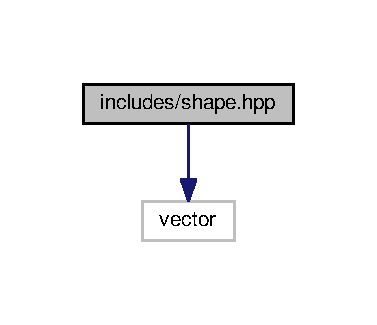
\includegraphics[width=181pt]{da/d73/shape_8hpp__incl}
\end{center}
\end{figure}
This graph shows which files directly or indirectly include this file\+:
\nopagebreak
\begin{figure}[H]
\begin{center}
\leavevmode
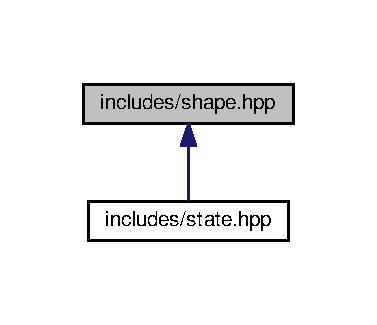
\includegraphics[width=181pt]{d8/d18/shape_8hpp__dep__incl}
\end{center}
\end{figure}
\subsection*{Classes}
\begin{DoxyCompactItemize}
\item 
class \hyperlink{classshape__type}{shape\+\_\+type}
\item 
class \hyperlink{classshape__2d}{shape\+\_\+2d}
\item 
class \hyperlink{classshape__3d}{shape\+\_\+3d}
\item 
class \hyperlink{classweibull}{weibull}
\item 
class \hyperlink{classsquare}{square}
\item 
class \hyperlink{classcube}{cube}
\item 
class \hyperlink{classsh__cluster}{sh\+\_\+cluster}
\end{DoxyCompactItemize}

\hypertarget{state_8hpp}{}\section{includes/state.hpp File Reference}
\label{state_8hpp}\index{includes/state.\+hpp@{includes/state.\+hpp}}
{\ttfamily \#include \char`\"{}param\+\_\+read.\+hpp\char`\"{}}\\*
{\ttfamily \#include \char`\"{}field\+\_\+type.\+hpp\char`\"{}}\\*
{\ttfamily \#include \char`\"{}thermodynamics.\+hpp\char`\"{}}\\*
{\ttfamily \#include \char`\"{}shape.\+hpp\char`\"{}}\\*
{\ttfamily \#include $<$string.\+h$>$}\\*
{\ttfamily \#include $<$vector$>$}\\*
Include dependency graph for state.\+hpp\+:\nopagebreak
\begin{figure}[H]
\begin{center}
\leavevmode
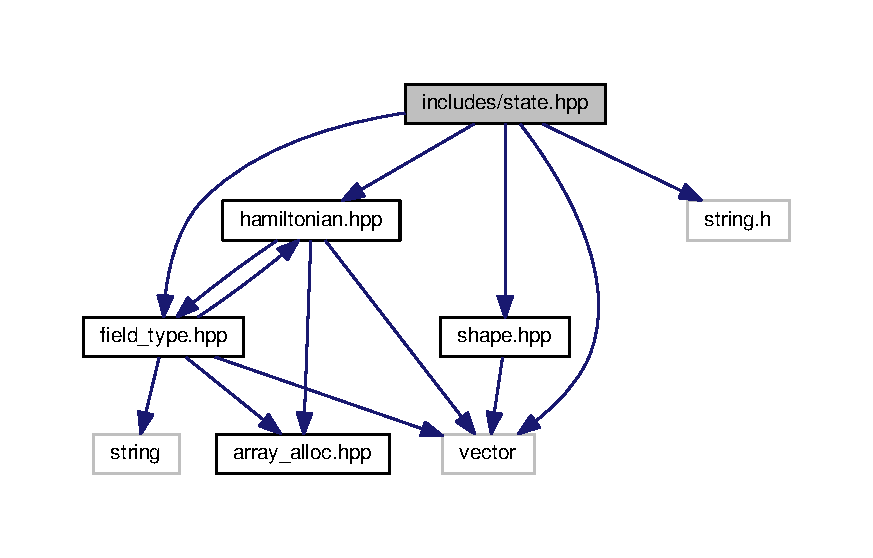
\includegraphics[width=350pt]{d0/dad/state_8hpp__incl}
\end{center}
\end{figure}
\subsection*{Classes}
\begin{DoxyCompactItemize}
\item 
class \hyperlink{classstate}{state}
\end{DoxyCompactItemize}

\hypertarget{stdrand_8hpp}{}\section{includes/stdrand.hpp File Reference}
\label{stdrand_8hpp}\index{includes/stdrand.\+hpp@{includes/stdrand.\+hpp}}
{\ttfamily \#include \char`\"{}xoroshiro128.\+hpp\char`\"{}}\\*
{\ttfamily \#include $<$random$>$}\\*
Include dependency graph for stdrand.\+hpp\+:
\nopagebreak
\begin{figure}[H]
\begin{center}
\leavevmode
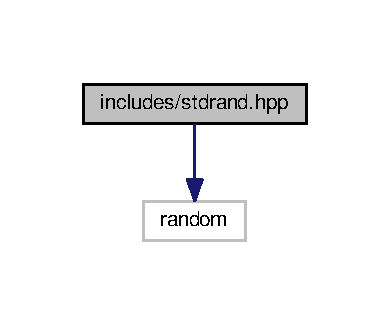
\includegraphics[width=258pt]{da/dbb/stdrand_8hpp__incl}
\end{center}
\end{figure}
\subsection*{Classes}
\begin{DoxyCompactItemize}
\item 
class \hyperlink{classstdrand_1_1std__randbase}{stdrand\+::std\+\_\+randbase}
\begin{DoxyCompactList}\small\item\em Base class for the random number generators. \end{DoxyCompactList}\item 
class \hyperlink{classstdrand_1_1std__d__unirand}{stdrand\+::std\+\_\+d\+\_\+unirand}
\begin{DoxyCompactList}\small\item\em Generator for uniform numbers between 0 and 1. \end{DoxyCompactList}\item 
class \hyperlink{classstdrand_1_1std__i__unirand}{stdrand\+::std\+\_\+i\+\_\+unirand}
\begin{DoxyCompactList}\small\item\em Generator for uniform integers between 0 and 1. \end{DoxyCompactList}\item 
class \hyperlink{classstdrand_1_1std__normrand}{stdrand\+::std\+\_\+normrand}
\begin{DoxyCompactList}\small\item\em Generator for random numbers on a normal distribution. \end{DoxyCompactList}\item 
class \hyperlink{classstdrand_1_1std__lognormrand}{stdrand\+::std\+\_\+lognormrand}
\begin{DoxyCompactList}\small\item\em Generator for random numbers on a lognormal distribution. \end{DoxyCompactList}\end{DoxyCompactItemize}
\subsection*{Namespaces}
\begin{DoxyCompactItemize}
\item 
 \hyperlink{namespacestdrand}{stdrand}
\end{DoxyCompactItemize}

\hypertarget{thermodynamics_8hpp}{}\section{includes/thermodynamics.hpp File Reference}
\label{thermodynamics_8hpp}\index{includes/thermodynamics.\+hpp@{includes/thermodynamics.\+hpp}}
{\ttfamily \#include \char`\"{}field\+\_\+type.\+hpp\char`\"{}}\\*
{\ttfamily \#include $<$vector$>$}\\*
{\ttfamily \#include $<$functional$>$}\\*
Include dependency graph for thermodynamics.\+hpp\+:\nopagebreak
\begin{figure}[H]
\begin{center}
\leavevmode
\includegraphics[width=300pt]{df/d3f/thermodynamics_8hpp__incl}
\end{center}
\end{figure}
This graph shows which files directly or indirectly include this file\+:\nopagebreak
\begin{figure}[H]
\begin{center}
\leavevmode
\includegraphics[width=226pt]{d0/d8f/thermodynamics_8hpp__dep__incl}
\end{center}
\end{figure}
\subsection*{Classes}
\begin{DoxyCompactItemize}
\item 
class \hyperlink{classparticle_1_1td_1_1functionObject}{particle\+::td\+::function\+Object}
\end{DoxyCompactItemize}
\subsection*{Namespaces}
\begin{DoxyCompactItemize}
\item 
 \hyperlink{namespaceparticle}{particle}
\item 
 \hyperlink{namespaceparticle_1_1td}{particle\+::td}
\end{DoxyCompactItemize}
\subsection*{Functions}
\begin{DoxyCompactItemize}
\item 
double \hyperlink{namespaceparticle_1_1td_a2967e054de9a7aa8d89d19ae1e920f69}{particle\+::td\+::solid\+\_\+angle} (const xt\+::xtensorf$<$ double, xt\+::xshape$<$ 4 $>$$>$ \&s1, const xt\+::xtensorf$<$ double, xt\+::xshape$<$ 4 $>$$>$ \&s2, const xt\+::xtensorf$<$ double, xt\+::xshape$<$ 4 $>$$>$ \&s3)
\end{DoxyCompactItemize}

\hypertarget{xoroshiro128_8hpp}{}\section{includes/xoroshiro128.hpp File Reference}
\label{xoroshiro128_8hpp}\index{includes/xoroshiro128.\+hpp@{includes/xoroshiro128.\+hpp}}
{\ttfamily \#include $<$cstdint$>$}\\*
{\ttfamily \#include $<$random$>$}\\*
{\ttfamily \#include $<$thread$>$}\\*
Include dependency graph for xoroshiro128.\+hpp\+:
\nopagebreak
\begin{figure}[H]
\begin{center}
\leavevmode
\includegraphics[width=256pt]{da/d39/xoroshiro128_8hpp__incl}
\end{center}
\end{figure}
This graph shows which files directly or indirectly include this file\+:
\nopagebreak
\begin{figure}[H]
\begin{center}
\leavevmode
\includegraphics[width=210pt]{d9/de3/xoroshiro128_8hpp__dep__incl}
\end{center}
\end{figure}
\subsection*{Classes}
\begin{DoxyCompactItemize}
\item 
struct \hyperlink{structrng_1_1tsc__seed}{rng\+::tsc\+\_\+seed}
\item 
struct \hyperlink{structrng_1_1random__device__seed}{rng\+::random\+\_\+device\+\_\+seed}
\item 
struct \hyperlink{structrng_1_1rng64}{rng\+::rng64}
\item 
struct \hyperlink{structrng_1_1rng128}{rng\+::rng128}
\end{DoxyCompactItemize}
\subsection*{Namespaces}
\begin{DoxyCompactItemize}
\item 
 \hyperlink{namespacerng}{rng}
\end{DoxyCompactItemize}
\subsection*{Macros}
\begin{DoxyCompactItemize}
\item 
\#define \hyperlink{xoroshiro128_8hpp_af25863dd4b1bcea5cdd7d809aa5ae10c}{R\+N\+G\+\_\+H}
\end{DoxyCompactItemize}


\subsection{Macro Definition Documentation}
\index{xoroshiro128.\+hpp@{xoroshiro128.\+hpp}!R\+N\+G\+\_\+H@{R\+N\+G\+\_\+H}}
\index{R\+N\+G\+\_\+H@{R\+N\+G\+\_\+H}!xoroshiro128.\+hpp@{xoroshiro128.\+hpp}}
\subsubsection[{\texorpdfstring{R\+N\+G\+\_\+H}{RNG_H}}]{\setlength{\rightskip}{0pt plus 5cm}\#define R\+N\+G\+\_\+H}\hypertarget{xoroshiro128_8hpp_af25863dd4b1bcea5cdd7d809aa5ae10c}{}\label{xoroshiro128_8hpp_af25863dd4b1bcea5cdd7d809aa5ae10c}

\hypertarget{README_8md}{}\section{R\+E\+A\+D\+M\+E.\+md File Reference}
\label{README_8md}\index{R\+E\+A\+D\+M\+E.\+md@{R\+E\+A\+D\+M\+E.\+md}}

%--- End generated contents ---

% Index
\backmatter
\newpage
\phantomsection
\clearemptydoublepage
\addcontentsline{toc}{chapter}{Index}
\printindex

\end{document}
